\documentclass[twoside]{book}

% Packages required by doxygen
\usepackage{calc}
\usepackage{doxygen}
\usepackage{graphicx}
\usepackage[utf8]{inputenc}
\usepackage{makeidx}
\usepackage{multicol}
\usepackage{multirow}
\usepackage{textcomp}
\usepackage[table]{xcolor}

% Font selection
\usepackage[T1]{fontenc}
\usepackage{mathptmx}
\usepackage[scaled=.90]{helvet}
\usepackage{courier}
\usepackage{amssymb}
\usepackage{sectsty}
\renewcommand{\familydefault}{\sfdefault}
\allsectionsfont{%
  \fontseries{bc}\selectfont%
  \color{darkgray}%
}
\renewcommand{\DoxyLabelFont}{%
  \fontseries{bc}\selectfont%
  \color{darkgray}%
}

% Page & text layout
\usepackage{geometry}
\geometry{%
  a4paper,%
  top=2.5cm,%
  bottom=2.5cm,%
  left=2.5cm,%
  right=2.5cm%
}
\tolerance=750
\hfuzz=15pt
\hbadness=750
\setlength{\emergencystretch}{15pt}
\setlength{\parindent}{0cm}
\setlength{\parskip}{0.2cm}
\makeatletter
\renewcommand{\paragraph}{%
  \@startsection{paragraph}{4}{0ex}{-1.0ex}{1.0ex}{%
    \normalfont\normalsize\bfseries\SS@parafont%
  }%
}
\renewcommand{\subparagraph}{%
  \@startsection{subparagraph}{5}{0ex}{-1.0ex}{1.0ex}{%
    \normalfont\normalsize\bfseries\SS@subparafont%
  }%
}
\makeatother

% Headers & footers
\usepackage{fancyhdr}
\pagestyle{fancyplain}
\fancyhead[LE]{\fancyplain{}{\bfseries\thepage}}
\fancyhead[CE]{\fancyplain{}{}}
\fancyhead[RE]{\fancyplain{}{\bfseries\leftmark}}
\fancyhead[LO]{\fancyplain{}{\bfseries\rightmark}}
\fancyhead[CO]{\fancyplain{}{}}
\fancyhead[RO]{\fancyplain{}{\bfseries\thepage}}
\fancyfoot[LE]{\fancyplain{}{}}
\fancyfoot[CE]{\fancyplain{}{}}
\fancyfoot[RE]{\fancyplain{}{\bfseries\scriptsize Generated on Wed May 21 2014 15\-:10\-:45 for Scrabble by Doxygen }}
\fancyfoot[LO]{\fancyplain{}{\bfseries\scriptsize Generated on Wed May 21 2014 15\-:10\-:45 for Scrabble by Doxygen }}
\fancyfoot[CO]{\fancyplain{}{}}
\fancyfoot[RO]{\fancyplain{}{}}
\renewcommand{\footrulewidth}{0.4pt}
\renewcommand{\chaptermark}[1]{%
  \markboth{#1}{}%
}
\renewcommand{\sectionmark}[1]{%
  \markright{\thesection\ #1}%
}

% Indices & bibliography
\usepackage{natbib}
\usepackage[titles]{tocloft}
\setcounter{tocdepth}{3}
\setcounter{secnumdepth}{5}
\makeindex

% Hyperlinks (required, but should be loaded last)
\usepackage{ifpdf}
\ifpdf
  \usepackage[pdftex,pagebackref=true]{hyperref}
\else
  \usepackage[ps2pdf,pagebackref=true]{hyperref}
\fi
\hypersetup{%
  colorlinks=true,%
  linkcolor=blue,%
  citecolor=blue,%
  unicode%
}

% Custom commands
\newcommand{\clearemptydoublepage}{%
  \newpage{\pagestyle{empty}\cleardoublepage}%
}


%===== C O N T E N T S =====

\begin{document}

% Titlepage & ToC
\hypersetup{pageanchor=false}
\pagenumbering{roman}
\begin{titlepage}
\vspace*{7cm}
\begin{center}%
{\Large Scrabble \\[1ex]\large 2.\-0 }\\
\vspace*{1cm}
{\large Generated by Doxygen 1.8.6}\\
\vspace*{0.5cm}
{\small Wed May 21 2014 15:10:45}\\
\end{center}
\end{titlepage}
\clearemptydoublepage
\tableofcontents
\clearemptydoublepage
\pagenumbering{arabic}
\hypersetup{pageanchor=true}

%--- Begin generated contents ---
\chapter{Data Structure Index}
\section{Data Structures}
Here are the data structures with brief descriptions\-:\begin{DoxyCompactList}
\item\contentsline{section}{\hyperlink{struct_case}{Case} }{\pageref{struct_case}}{}
\item\contentsline{section}{\hyperlink{structelement}{element} }{\pageref{structelement}}{}
\item\contentsline{section}{\hyperlink{struct_image_cliquable}{Image\-Cliquable} }{\pageref{struct_image_cliquable}}{}
\item\contentsline{section}{\hyperlink{struct_jeton}{Jeton} }{\pageref{struct_jeton}}{}
\end{DoxyCompactList}

\chapter{File Index}
\section{File List}
Here is a list of all files with brief descriptions\-:\begin{DoxyCompactList}
\item\contentsline{section}{/home/r40u1/\-P\-I/\-Scrabble\-\_\-final/headers/\hyperlink{defausse_8h}{defausse.\-h} }{\pageref{defausse_8h}}{}
\item\contentsline{section}{/home/r40u1/\-P\-I/\-Scrabble\-\_\-final/headers/\hyperlink{distribution_8h}{distribution.\-h} }{\pageref{distribution_8h}}{}
\item\contentsline{section}{/home/r40u1/\-P\-I/\-Scrabble\-\_\-final/headers/\hyperlink{est_dans_dico_8h}{est\-Dans\-Dico.\-h} }{\pageref{est_dans_dico_8h}}{}
\item\contentsline{section}{/home/r40u1/\-P\-I/\-Scrabble\-\_\-final/headers/\hyperlink{grille_8h}{grille.\-h} }{\pageref{grille_8h}}{}
\item\contentsline{section}{/home/r40u1/\-P\-I/\-Scrabble\-\_\-final/headers/\hyperlink{interface_8h}{interface.\-h} }{\pageref{interface_8h}}{}
\item\contentsline{section}{/home/r40u1/\-P\-I/\-Scrabble\-\_\-final/headers/\hyperlink{parcours_mots_crees_8h}{parcours\-Mots\-Crees.\-h} }{\pageref{parcours_mots_crees_8h}}{}
\item\contentsline{section}{/home/r40u1/\-P\-I/\-Scrabble\-\_\-final/headers/\hyperlink{pile_8h}{pile.\-h} }{\pageref{pile_8h}}{}
\item\contentsline{section}{/home/r40u1/\-P\-I/\-Scrabble\-\_\-final/headers/\hyperlink{verif_masque_grille_8h}{verif\-Masque\-Grille.\-h} }{\pageref{verif_masque_grille_8h}}{}
\item\contentsline{section}{\hyperlink{structure_de_donnee_8h}{structure\-De\-Donnee.\-h} }{\pageref{structure_de_donnee_8h}}{}
\item\contentsline{section}{/home/r40u1/\-P\-I/\-Scrabble\-\_\-final/sources/\hyperlink{defausse_8c}{defausse.\-c} }{\pageref{defausse_8c}}{}
\item\contentsline{section}{/home/r40u1/\-P\-I/\-Scrabble\-\_\-final/sources/\hyperlink{distribution_8c}{distribution.\-c} }{\pageref{distribution_8c}}{}
\item\contentsline{section}{/home/r40u1/\-P\-I/\-Scrabble\-\_\-final/sources/\hyperlink{est_dans_dico_8c}{est\-Dans\-Dico.\-c} }{\pageref{est_dans_dico_8c}}{}
\item\contentsline{section}{/home/r40u1/\-P\-I/\-Scrabble\-\_\-final/sources/\hyperlink{grille_8c}{grille.\-c} }{\pageref{grille_8c}}{}
\item\contentsline{section}{/home/r40u1/\-P\-I/\-Scrabble\-\_\-final/sources/\hyperlink{interface_8c}{interface.\-c} }{\pageref{interface_8c}}{}
\item\contentsline{section}{/home/r40u1/\-P\-I/\-Scrabble\-\_\-final/sources/\hyperlink{parcours_mots_crees_8c}{parcours\-Mots\-Crees.\-c} }{\pageref{parcours_mots_crees_8c}}{}
\item\contentsline{section}{/home/r40u1/\-P\-I/\-Scrabble\-\_\-final/sources/\hyperlink{pile_8c}{pile.\-c} }{\pageref{pile_8c}}{}
\item\contentsline{section}{/home/r40u1/\-P\-I/\-Scrabble\-\_\-final/sources/\hyperlink{test_defausse_8c}{test\-Defausse.\-c} }{\pageref{test_defausse_8c}}{}
\item\contentsline{section}{/home/r40u1/\-P\-I/\-Scrabble\-\_\-final/sources/\hyperlink{test_distribution_8c}{test\-Distribution.\-c} }{\pageref{test_distribution_8c}}{}
\item\contentsline{section}{/home/r40u1/\-P\-I/\-Scrabble\-\_\-final/sources/\hyperlink{test_est_dans_dico_8c}{test\-Est\-Dans\-Dico.\-c} }{\pageref{test_est_dans_dico_8c}}{}
\item\contentsline{section}{/home/r40u1/\-P\-I/\-Scrabble\-\_\-final/sources/\hyperlink{test_grille_8c}{test\-Grille.\-c} }{\pageref{test_grille_8c}}{}
\item\contentsline{section}{/home/r40u1/\-P\-I/\-Scrabble\-\_\-final/sources/\hyperlink{verif_masque_grille_8c}{verif\-Masque\-Grille.\-c} }{\pageref{verif_masque_grille_8c}}{}
\end{DoxyCompactList}

\chapter{Data Structure Documentation}
\hypertarget{struct_case}{\section{Case Struct Reference}
\label{struct_case}\index{Case@{Case}}
}


{\ttfamily \#include $<$structure\-De\-Donnee.\-h$>$}



Collaboration diagram for Case\-:\nopagebreak
\begin{figure}[H]
\begin{center}
\leavevmode
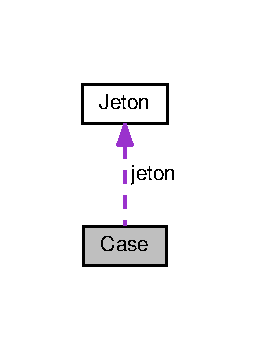
\includegraphics[width=125pt]{struct_case__coll__graph}
\end{center}
\end{figure}
\subsection*{Data Fields}
\begin{DoxyCompactItemize}
\item 
struct \hyperlink{struct_jeton}{Jeton} \hyperlink{struct_case_a9f4b5819c5c0a86e2652b81fef1daada}{jeton}
\item 
int \hyperlink{struct_case_a221f7ea49ba6862c68e57d4f3771d649}{multi\-Mot}
\item 
int \hyperlink{struct_case_a6f17e7aa98aefcb66a93b9933e3eb107}{multi\-Lettre}
\end{DoxyCompactItemize}


\subsection{Field Documentation}
\hypertarget{struct_case_a9f4b5819c5c0a86e2652b81fef1daada}{\index{Case@{Case}!jeton@{jeton}}
\index{jeton@{jeton}!Case@{Case}}
\subsubsection[{jeton}]{\setlength{\rightskip}{0pt plus 5cm}struct {\bf Jeton} jeton}}\label{struct_case_a9f4b5819c5c0a86e2652b81fef1daada}
\hypertarget{struct_case_a6f17e7aa98aefcb66a93b9933e3eb107}{\index{Case@{Case}!multi\-Lettre@{multi\-Lettre}}
\index{multi\-Lettre@{multi\-Lettre}!Case@{Case}}
\subsubsection[{multi\-Lettre}]{\setlength{\rightskip}{0pt plus 5cm}int multi\-Lettre}}\label{struct_case_a6f17e7aa98aefcb66a93b9933e3eb107}
\hypertarget{struct_case_a221f7ea49ba6862c68e57d4f3771d649}{\index{Case@{Case}!multi\-Mot@{multi\-Mot}}
\index{multi\-Mot@{multi\-Mot}!Case@{Case}}
\subsubsection[{multi\-Mot}]{\setlength{\rightskip}{0pt plus 5cm}int multi\-Mot}}\label{struct_case_a221f7ea49ba6862c68e57d4f3771d649}


The documentation for this struct was generated from the following file\-:\begin{DoxyCompactItemize}
\item 
\hyperlink{structure_de_donnee_8h}{structure\-De\-Donnee.\-h}\end{DoxyCompactItemize}

\hypertarget{structelement}{\section{element Struct Reference}
\label{structelement}\index{element@{element}}
}


{\ttfamily \#include $<$structure\-De\-Donnee.\-h$>$}



Collaboration diagram for element\-:\nopagebreak
\begin{figure}[H]
\begin{center}
\leavevmode
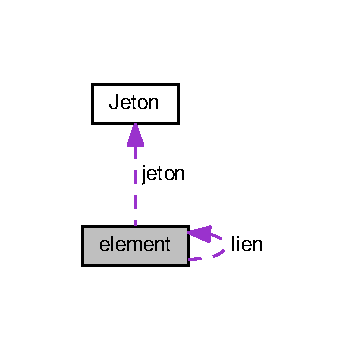
\includegraphics[width=167pt]{structelement__coll__graph}
\end{center}
\end{figure}
\subsection*{Data Fields}
\begin{DoxyCompactItemize}
\item 
\hyperlink{struct_jeton}{Jeton} \hyperlink{structelement_ad1f18dda3e603c8cf6c98ee549208114}{jeton}
\item 
struct \hyperlink{structelement}{element} $\ast$ \hyperlink{structelement_a15a89fdc2b7a3c54ea8628e307925c89}{lien}
\end{DoxyCompactItemize}


\subsection{Field Documentation}
\hypertarget{structelement_ad1f18dda3e603c8cf6c98ee549208114}{\index{element@{element}!jeton@{jeton}}
\index{jeton@{jeton}!element@{element}}
\subsubsection[{jeton}]{\setlength{\rightskip}{0pt plus 5cm}{\bf Jeton} jeton}}\label{structelement_ad1f18dda3e603c8cf6c98ee549208114}
\hypertarget{structelement_a15a89fdc2b7a3c54ea8628e307925c89}{\index{element@{element}!lien@{lien}}
\index{lien@{lien}!element@{element}}
\subsubsection[{lien}]{\setlength{\rightskip}{0pt plus 5cm}struct {\bf element}$\ast$ lien}}\label{structelement_a15a89fdc2b7a3c54ea8628e307925c89}


The documentation for this struct was generated from the following file\-:\begin{DoxyCompactItemize}
\item 
\hyperlink{structure_de_donnee_8h}{structure\-De\-Donnee.\-h}\end{DoxyCompactItemize}

\hypertarget{struct_image_cliquable}{\section{Image\-Cliquable Struct Reference}
\label{struct_image_cliquable}\index{Image\-Cliquable@{Image\-Cliquable}}
}


{\ttfamily \#include $<$interface.\-h$>$}

\subsection*{Data Fields}
\begin{DoxyCompactItemize}
\item 
Gtk\-Widget $\ast$ \hyperlink{struct_image_cliquable_ab419ba2026044cab0230a07a27b30a1c}{p\-Button}
\item 
Gtk\-Widget $\ast$ \hyperlink{struct_image_cliquable_a9c81ae9ebe0645f6eadabbb372b0f1bb}{p\-Image}
\end{DoxyCompactItemize}


\subsection{Field Documentation}
\hypertarget{struct_image_cliquable_ab419ba2026044cab0230a07a27b30a1c}{\index{Image\-Cliquable@{Image\-Cliquable}!p\-Button@{p\-Button}}
\index{p\-Button@{p\-Button}!ImageCliquable@{Image\-Cliquable}}
\subsubsection[{p\-Button}]{\setlength{\rightskip}{0pt plus 5cm}Gtk\-Widget$\ast$ p\-Button}}\label{struct_image_cliquable_ab419ba2026044cab0230a07a27b30a1c}
\hypertarget{struct_image_cliquable_a9c81ae9ebe0645f6eadabbb372b0f1bb}{\index{Image\-Cliquable@{Image\-Cliquable}!p\-Image@{p\-Image}}
\index{p\-Image@{p\-Image}!ImageCliquable@{Image\-Cliquable}}
\subsubsection[{p\-Image}]{\setlength{\rightskip}{0pt plus 5cm}Gtk\-Widget$\ast$ p\-Image}}\label{struct_image_cliquable_a9c81ae9ebe0645f6eadabbb372b0f1bb}


The documentation for this struct was generated from the following file\-:\begin{DoxyCompactItemize}
\item 
/home/r40u1/\-P\-I/\-Scrabble\-\_\-final/headers/\hyperlink{interface_8h}{interface.\-h}\end{DoxyCompactItemize}

\hypertarget{struct_jeton}{\section{Jeton Struct Reference}
\label{struct_jeton}\index{Jeton@{Jeton}}
}


{\ttfamily \#include $<$structure\-De\-Donnee.\-h$>$}

\subsection*{Data Fields}
\begin{DoxyCompactItemize}
\item 
char \hyperlink{struct_jeton_a1fd1cee5d78e1f4af4a8fe512320ef95}{lettre}
\item 
int \hyperlink{struct_jeton_a8e030c012e3b74a6d076739c4c7ecb69}{valeur}
\end{DoxyCompactItemize}


\subsection{Field Documentation}
\hypertarget{struct_jeton_a1fd1cee5d78e1f4af4a8fe512320ef95}{\index{Jeton@{Jeton}!lettre@{lettre}}
\index{lettre@{lettre}!Jeton@{Jeton}}
\subsubsection[{lettre}]{\setlength{\rightskip}{0pt plus 5cm}char lettre}}\label{struct_jeton_a1fd1cee5d78e1f4af4a8fe512320ef95}
\hypertarget{struct_jeton_a8e030c012e3b74a6d076739c4c7ecb69}{\index{Jeton@{Jeton}!valeur@{valeur}}
\index{valeur@{valeur}!Jeton@{Jeton}}
\subsubsection[{valeur}]{\setlength{\rightskip}{0pt plus 5cm}int valeur}}\label{struct_jeton_a8e030c012e3b74a6d076739c4c7ecb69}


The documentation for this struct was generated from the following file\-:\begin{DoxyCompactItemize}
\item 
\hyperlink{structure_de_donnee_8h}{structure\-De\-Donnee.\-h}\end{DoxyCompactItemize}

\chapter{File Documentation}
\hypertarget{defausse_8h}{\section{/home/r40u1/\-P\-I/\-Scrabble\-\_\-final/headers/defausse.h File Reference}
\label{defausse_8h}\index{/home/r40u1/\-P\-I/\-Scrabble\-\_\-final/headers/defausse.\-h@{/home/r40u1/\-P\-I/\-Scrabble\-\_\-final/headers/defausse.\-h}}
}
This graph shows which files directly or indirectly include this file\-:\nopagebreak
\begin{figure}[H]
\begin{center}
\leavevmode
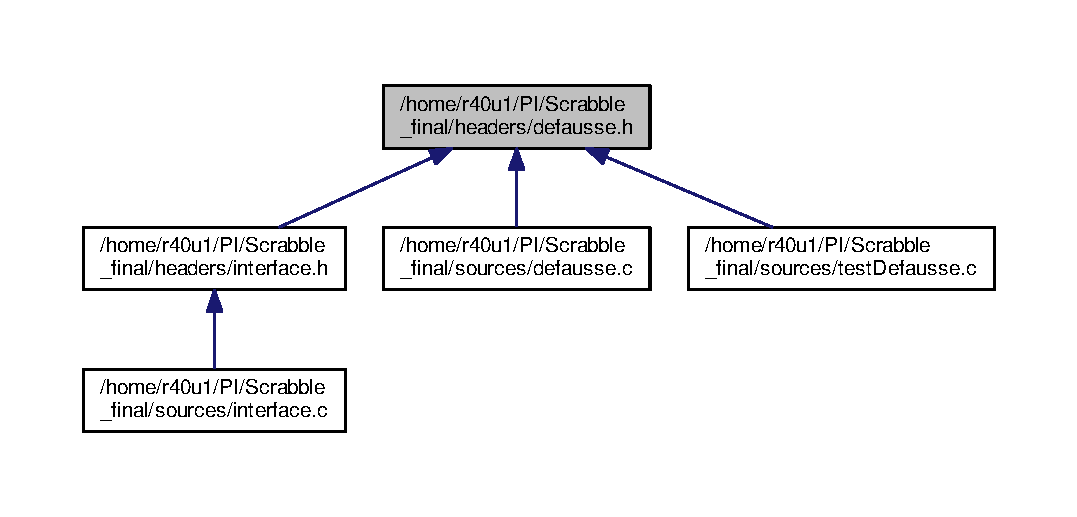
\includegraphics[width=350pt]{defausse_8h__dep__incl}
\end{center}
\end{figure}
\subsection*{Functions}
\begin{DoxyCompactItemize}
\item 
void \hyperlink{defausse_8h_aad62c2486092c0fc1d0a7a8a760ecc74}{defausse} (\hyperlink{structure_de_donnee_8h_abde700801ddcd10c40bdf389ff5b1494}{Chevalet} chevalet, \hyperlink{structure_de_donnee_8h_aeb2e4c1daa2de38a0efbf9ab87674140}{Pile} $\ast$\hyperlink{interface_8c_a6d4f2018c7ae823808170f38d6f18608}{p\-Pioche}, char lettres\-A\-Deffausser\mbox{[}7\mbox{]})
\item 
void \hyperlink{defausse_8h_a3eac94981c9152c6a158c57dd6d596e9}{defausse\-Par\-Indice} (\hyperlink{structure_de_donnee_8h_abde700801ddcd10c40bdf389ff5b1494}{Chevalet} chevalet, \hyperlink{structure_de_donnee_8h_aeb2e4c1daa2de38a0efbf9ab87674140}{Pile} $\ast$\hyperlink{interface_8c_a6d4f2018c7ae823808170f38d6f18608}{p\-Pioche}, int \hyperlink{interface_8c_afeef952dff3f63f7fb13ef662475b286}{masque\-Defausse}\mbox{[}$\,$\mbox{]})
\end{DoxyCompactItemize}


\subsection{Function Documentation}
\hypertarget{defausse_8h_aad62c2486092c0fc1d0a7a8a760ecc74}{\index{defausse.\-h@{defausse.\-h}!defausse@{defausse}}
\index{defausse@{defausse}!defausse.h@{defausse.\-h}}
\subsubsection[{defausse}]{\setlength{\rightskip}{0pt plus 5cm}void defausse (
\begin{DoxyParamCaption}
\item[{{\bf Chevalet}}]{chevalet, }
\item[{{\bf Pile} $\ast$}]{p\-Pioche, }
\item[{char}]{lettres\-A\-Deffausser\mbox{[}7\mbox{]}}
\end{DoxyParamCaption}
)}}\label{defausse_8h_aad62c2486092c0fc1d0a7a8a760ecc74}
\hypertarget{defausse_8h_a3eac94981c9152c6a158c57dd6d596e9}{\index{defausse.\-h@{defausse.\-h}!defausse\-Par\-Indice@{defausse\-Par\-Indice}}
\index{defausse\-Par\-Indice@{defausse\-Par\-Indice}!defausse.h@{defausse.\-h}}
\subsubsection[{defausse\-Par\-Indice}]{\setlength{\rightskip}{0pt plus 5cm}void defausse\-Par\-Indice (
\begin{DoxyParamCaption}
\item[{{\bf Chevalet}}]{chevalet, }
\item[{{\bf Pile} $\ast$}]{p\-Pioche, }
\item[{int}]{masque\-Defausse\mbox{[}$\,$\mbox{]}}
\end{DoxyParamCaption}
)}}\label{defausse_8h_a3eac94981c9152c6a158c57dd6d596e9}

\hypertarget{distribution_8h}{\section{/home/r40u1/\-P\-I/\-Scrabble\-\_\-final/headers/distribution.h File Reference}
\label{distribution_8h}\index{/home/r40u1/\-P\-I/\-Scrabble\-\_\-final/headers/distribution.\-h@{/home/r40u1/\-P\-I/\-Scrabble\-\_\-final/headers/distribution.\-h}}
}
This graph shows which files directly or indirectly include this file\-:\nopagebreak
\begin{figure}[H]
\begin{center}
\leavevmode
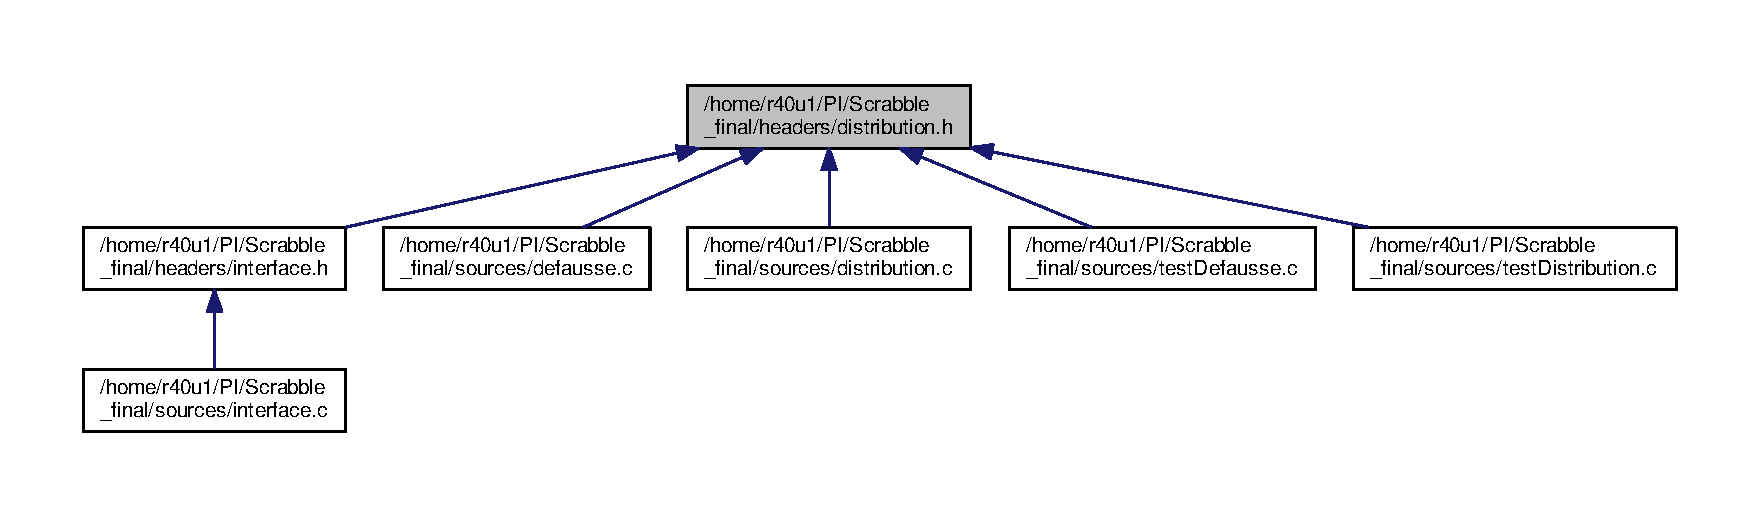
\includegraphics[width=350pt]{distribution_8h__dep__incl}
\end{center}
\end{figure}
\subsection*{Functions}
\begin{DoxyCompactItemize}
\item 
void \hyperlink{distribution_8h_a5a28ffd4625fd10849dac9bde2f695b2}{generation\-Ensemble\-Des\-Jetons} (\hyperlink{struct_jeton}{Jeton} ensemble\-Des\-Jetons\mbox{[}\hyperlink{structure_de_donnee_8h_a71e2e07f0ea54740cb5421e00e77a979}{N\-O\-M\-B\-R\-E\-D\-E\-J\-E\-T\-O\-N}\mbox{]})
\item 
void \hyperlink{distribution_8h_a7d8b638fa86c3426d190350cf0017e33}{empilage\-Aleatoire\-Jeton} (\hyperlink{struct_jeton}{Jeton} ensemble\-Des\-Jetons\mbox{[}\hyperlink{structure_de_donnee_8h_a71e2e07f0ea54740cb5421e00e77a979}{N\-O\-M\-B\-R\-E\-D\-E\-J\-E\-T\-O\-N}\mbox{]}, int nb\-Jetons\-Restants, \hyperlink{structure_de_donnee_8h_aeb2e4c1daa2de38a0efbf9ab87674140}{Pile} $\ast$\hyperlink{interface_8c_a6d4f2018c7ae823808170f38d6f18608}{p\-Pioche})
\item 
void \hyperlink{distribution_8h_aa56a67af62b835882c8455f7179391fb}{distribution\-Jetons} (\hyperlink{structure_de_donnee_8h_aeb2e4c1daa2de38a0efbf9ab87674140}{Pile} $\ast$\hyperlink{interface_8c_a6d4f2018c7ae823808170f38d6f18608}{p\-Pioche}, \hyperlink{struct_jeton}{Jeton} chevalet\mbox{[}7\mbox{]})
\item 
void \hyperlink{distribution_8h_ac3ed546272da04bab4c146d514c9f309}{distribution\-Initiale} (\hyperlink{struct_jeton}{Jeton} ensemble\-Des\-Jetons\mbox{[}\hyperlink{structure_de_donnee_8h_a71e2e07f0ea54740cb5421e00e77a979}{N\-O\-M\-B\-R\-E\-D\-E\-J\-E\-T\-O\-N}\mbox{]}, \hyperlink{structure_de_donnee_8h_aeb2e4c1daa2de38a0efbf9ab87674140}{Pile} $\ast$\hyperlink{interface_8c_a6d4f2018c7ae823808170f38d6f18608}{p\-Pioche}, \hyperlink{structure_de_donnee_8h_abde700801ddcd10c40bdf389ff5b1494}{Chevalet} ensemble\-Des\-Chevalets\mbox{[}$\,$\mbox{]}, int \hyperlink{interface_8c_a006645f5fca9c8be4a3a8a6398330060}{nb\-Joueurs})
\end{DoxyCompactItemize}


\subsection{Function Documentation}
\hypertarget{distribution_8h_ac3ed546272da04bab4c146d514c9f309}{\index{distribution.\-h@{distribution.\-h}!distribution\-Initiale@{distribution\-Initiale}}
\index{distribution\-Initiale@{distribution\-Initiale}!distribution.h@{distribution.\-h}}
\subsubsection[{distribution\-Initiale}]{\setlength{\rightskip}{0pt plus 5cm}void distribution\-Initiale (
\begin{DoxyParamCaption}
\item[{{\bf Jeton}}]{ensemble\-Des\-Jetons\mbox{[}\-N\-O\-M\-B\-R\-E\-D\-E\-J\-E\-T\-O\-N\mbox{]}, }
\item[{{\bf Pile} $\ast$}]{p\-Pioche, }
\item[{{\bf Chevalet}}]{ensemble\-Des\-Chevalets\mbox{[}$\,$\mbox{]}, }
\item[{int}]{nb\-Joueurs}
\end{DoxyParamCaption}
)}}\label{distribution_8h_ac3ed546272da04bab4c146d514c9f309}
Intitialisation des chevalets des joueurs (appel aux 3 fonctions précédentes) \hypertarget{distribution_8h_aa56a67af62b835882c8455f7179391fb}{\index{distribution.\-h@{distribution.\-h}!distribution\-Jetons@{distribution\-Jetons}}
\index{distribution\-Jetons@{distribution\-Jetons}!distribution.h@{distribution.\-h}}
\subsubsection[{distribution\-Jetons}]{\setlength{\rightskip}{0pt plus 5cm}void distribution\-Jetons (
\begin{DoxyParamCaption}
\item[{{\bf Pile} $\ast$}]{p\-Pioche, }
\item[{{\bf Chevalet}}]{chevalet}
\end{DoxyParamCaption}
)}}\label{distribution_8h_aa56a67af62b835882c8455f7179391fb}
On distribue le nombre de jetons nécessaires afin de compléter le chevalet du joueur \hypertarget{distribution_8h_a7d8b638fa86c3426d190350cf0017e33}{\index{distribution.\-h@{distribution.\-h}!empilage\-Aleatoire\-Jeton@{empilage\-Aleatoire\-Jeton}}
\index{empilage\-Aleatoire\-Jeton@{empilage\-Aleatoire\-Jeton}!distribution.h@{distribution.\-h}}
\subsubsection[{empilage\-Aleatoire\-Jeton}]{\setlength{\rightskip}{0pt plus 5cm}void empilage\-Aleatoire\-Jeton (
\begin{DoxyParamCaption}
\item[{{\bf Jeton}}]{ensemble\-Des\-Jetons\mbox{[}\-N\-O\-M\-B\-R\-E\-D\-E\-J\-E\-T\-O\-N\mbox{]}, }
\item[{int}]{nb\-Jetons\-Restants, }
\item[{{\bf Pile} $\ast$}]{p\-Pioche}
\end{DoxyParamCaption}
)}}\label{distribution_8h_a7d8b638fa86c3426d190350cf0017e33}
Les jetons du tableau sont empilés aléatoirement dans la pioche \hypertarget{distribution_8h_a5a28ffd4625fd10849dac9bde2f695b2}{\index{distribution.\-h@{distribution.\-h}!generation\-Ensemble\-Des\-Jetons@{generation\-Ensemble\-Des\-Jetons}}
\index{generation\-Ensemble\-Des\-Jetons@{generation\-Ensemble\-Des\-Jetons}!distribution.h@{distribution.\-h}}
\subsubsection[{generation\-Ensemble\-Des\-Jetons}]{\setlength{\rightskip}{0pt plus 5cm}void generation\-Ensemble\-Des\-Jetons (
\begin{DoxyParamCaption}
\item[{{\bf Jeton}}]{ensemble\-Des\-Jetons\mbox{[}\-N\-O\-M\-B\-R\-E\-D\-E\-J\-E\-T\-O\-N\mbox{]}}
\end{DoxyParamCaption}
)}}\label{distribution_8h_a5a28ffd4625fd10849dac9bde2f695b2}
Construction du tableau des jetons dans l'ordre alphabétique 
\hypertarget{est_dans_dico_8h}{\section{/home/r40u1/\-P\-I/\-Scrabble\-\_\-final/headers/est\-Dans\-Dico.h File Reference}
\label{est_dans_dico_8h}\index{/home/r40u1/\-P\-I/\-Scrabble\-\_\-final/headers/est\-Dans\-Dico.\-h@{/home/r40u1/\-P\-I/\-Scrabble\-\_\-final/headers/est\-Dans\-Dico.\-h}}
}
This graph shows which files directly or indirectly include this file\-:\nopagebreak
\begin{figure}[H]
\begin{center}
\leavevmode
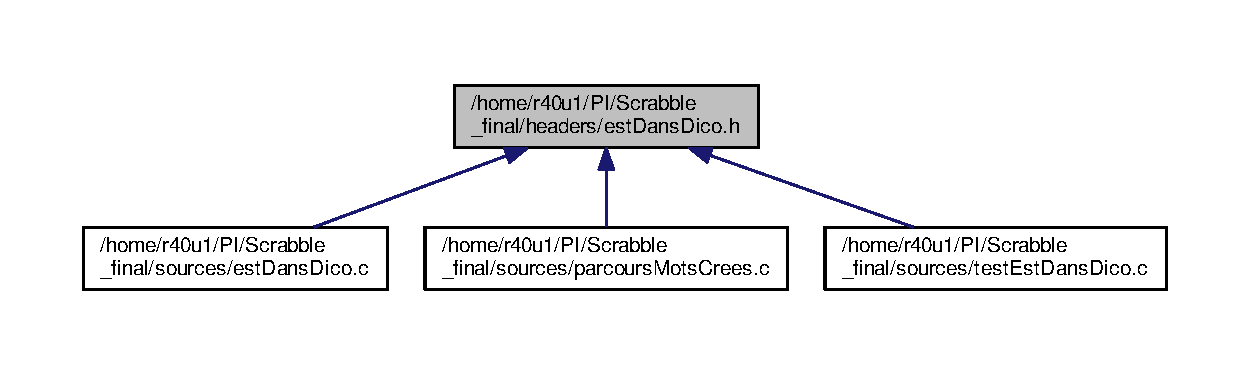
\includegraphics[width=350pt]{est_dans_dico_8h__dep__incl}
\end{center}
\end{figure}
\subsection*{Functions}
\begin{DoxyCompactItemize}
\item 
\hyperlink{structure_de_donnee_8h_a426c0d223e7dc6b87d723c4c0c0e1f58}{Booleen} \hyperlink{est_dans_dico_8h_a1e885dbf9866c7e930fd6eea00b8dd76}{comparer} (char $\ast$mot1, char $\ast$mot2)
\item 
\hyperlink{structure_de_donnee_8h_a426c0d223e7dc6b87d723c4c0c0e1f58}{Booleen} \hyperlink{est_dans_dico_8h_a3bcdca923df984cf2349d6074f2ce000}{est\-Dans\-Dico} (char $\ast$mot)
\end{DoxyCompactItemize}


\subsection{Function Documentation}
\hypertarget{est_dans_dico_8h_a1e885dbf9866c7e930fd6eea00b8dd76}{\index{est\-Dans\-Dico.\-h@{est\-Dans\-Dico.\-h}!comparer@{comparer}}
\index{comparer@{comparer}!estDansDico.h@{est\-Dans\-Dico.\-h}}
\subsubsection[{comparer}]{\setlength{\rightskip}{0pt plus 5cm}{\bf Booleen} comparer (
\begin{DoxyParamCaption}
\item[{char $\ast$}]{mot1, }
\item[{char $\ast$}]{mot2}
\end{DoxyParamCaption}
)}}\label{est_dans_dico_8h_a1e885dbf9866c7e930fd6eea00b8dd76}
retourne V\-R\-A\-I si les deux mots sont identiques \hypertarget{est_dans_dico_8h_a3bcdca923df984cf2349d6074f2ce000}{\index{est\-Dans\-Dico.\-h@{est\-Dans\-Dico.\-h}!est\-Dans\-Dico@{est\-Dans\-Dico}}
\index{est\-Dans\-Dico@{est\-Dans\-Dico}!estDansDico.h@{est\-Dans\-Dico.\-h}}
\subsubsection[{est\-Dans\-Dico}]{\setlength{\rightskip}{0pt plus 5cm}{\bf Booleen} est\-Dans\-Dico (
\begin{DoxyParamCaption}
\item[{char $\ast$}]{mot}
\end{DoxyParamCaption}
)}}\label{est_dans_dico_8h_a3bcdca923df984cf2349d6074f2ce000}
retourne V\-R\-A\-I si le mot se trouve dans le dictionnaire 
\hypertarget{grille_8h}{\section{/home/r40u1/\-P\-I/\-Scrabble\-\_\-final/headers/grille.h File Reference}
\label{grille_8h}\index{/home/r40u1/\-P\-I/\-Scrabble\-\_\-final/headers/grille.\-h@{/home/r40u1/\-P\-I/\-Scrabble\-\_\-final/headers/grille.\-h}}
}
This graph shows which files directly or indirectly include this file\-:\nopagebreak
\begin{figure}[H]
\begin{center}
\leavevmode
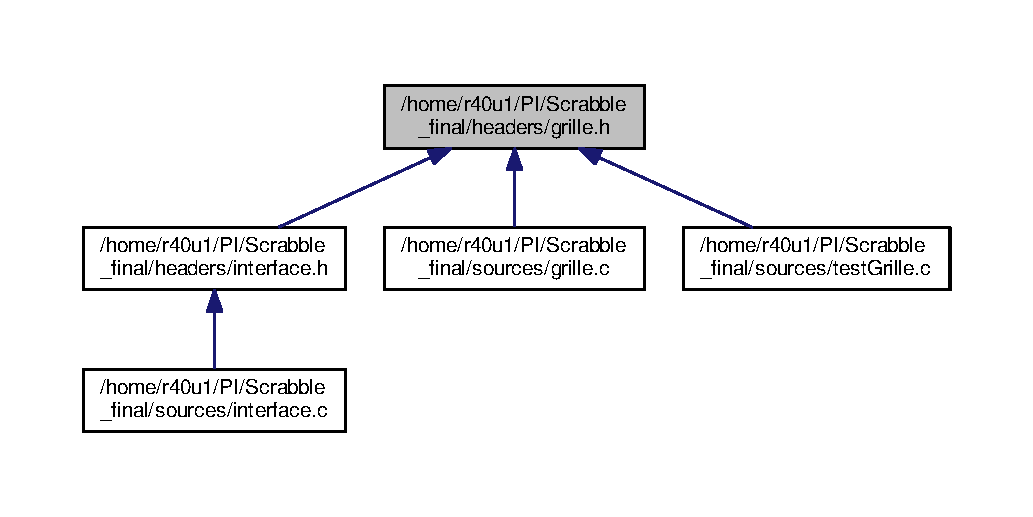
\includegraphics[width=350pt]{grille_8h__dep__incl}
\end{center}
\end{figure}
\subsection*{Functions}
\begin{DoxyCompactItemize}
\item 
void \hyperlink{grille_8h_aea9f328ee16f7d03cd836fa3cfb0d62a}{bonus\-Partiel} (\hyperlink{structure_de_donnee_8h_a4b19d9524b7f293ad87dd6bd9d121b25}{Grille} grille)
\item 
void \hyperlink{grille_8h_a9b2955f028d1c2fd61e5c0bf3c3c3a4d}{symetries} (\hyperlink{structure_de_donnee_8h_a4b19d9524b7f293ad87dd6bd9d121b25}{Grille} grille)
\item 
void \hyperlink{grille_8h_a1025b314e1127489285982e0c76d5b67}{afficher\-Grille} (\hyperlink{structure_de_donnee_8h_a4b19d9524b7f293ad87dd6bd9d121b25}{Grille} grille)
\item 
void \hyperlink{grille_8h_a21f7d6889dc7a0400edc3051a92a65ce}{generer\-Grille} (\hyperlink{structure_de_donnee_8h_a4b19d9524b7f293ad87dd6bd9d121b25}{Grille} $\ast$\hyperlink{interface_8c_a73ce74e635bbc82629b4ca70fea91eb2}{p\-Grille})
\end{DoxyCompactItemize}


\subsection{Function Documentation}
\hypertarget{grille_8h_a1025b314e1127489285982e0c76d5b67}{\index{grille.\-h@{grille.\-h}!afficher\-Grille@{afficher\-Grille}}
\index{afficher\-Grille@{afficher\-Grille}!grille.h@{grille.\-h}}
\subsubsection[{afficher\-Grille}]{\setlength{\rightskip}{0pt plus 5cm}void afficher\-Grille (
\begin{DoxyParamCaption}
\item[{{\bf Grille}}]{grille}
\end{DoxyParamCaption}
)}}\label{grille_8h_a1025b314e1127489285982e0c76d5b67}
affichage de la grille sur le terminal \hypertarget{grille_8h_aea9f328ee16f7d03cd836fa3cfb0d62a}{\index{grille.\-h@{grille.\-h}!bonus\-Partiel@{bonus\-Partiel}}
\index{bonus\-Partiel@{bonus\-Partiel}!grille.h@{grille.\-h}}
\subsubsection[{bonus\-Partiel}]{\setlength{\rightskip}{0pt plus 5cm}void bonus\-Partiel (
\begin{DoxyParamCaption}
\item[{{\bf Grille}}]{grille}
\end{DoxyParamCaption}
)}}\label{grille_8h_aea9f328ee16f7d03cd836fa3cfb0d62a}
Initialisation d'un premier huitième de la grille \hypertarget{grille_8h_a21f7d6889dc7a0400edc3051a92a65ce}{\index{grille.\-h@{grille.\-h}!generer\-Grille@{generer\-Grille}}
\index{generer\-Grille@{generer\-Grille}!grille.h@{grille.\-h}}
\subsubsection[{generer\-Grille}]{\setlength{\rightskip}{0pt plus 5cm}void generer\-Grille (
\begin{DoxyParamCaption}
\item[{{\bf Grille} $\ast$}]{p\-Grille}
\end{DoxyParamCaption}
)}}\label{grille_8h_a21f7d6889dc7a0400edc3051a92a65ce}
génère la grille (combinaison des deux fonctions précédentes \hypertarget{grille_8h_a9b2955f028d1c2fd61e5c0bf3c3c3a4d}{\index{grille.\-h@{grille.\-h}!symetries@{symetries}}
\index{symetries@{symetries}!grille.h@{grille.\-h}}
\subsubsection[{symetries}]{\setlength{\rightskip}{0pt plus 5cm}void symetries (
\begin{DoxyParamCaption}
\item[{{\bf Grille}}]{grille}
\end{DoxyParamCaption}
)}}\label{grille_8h_a9b2955f028d1c2fd61e5c0bf3c3c3a4d}
Obtention de la grille entière par symétries 
\hypertarget{interface_8h}{\section{/home/r40u1/\-P\-I/\-Scrabble\-\_\-final/headers/interface.h File Reference}
\label{interface_8h}\index{/home/r40u1/\-P\-I/\-Scrabble\-\_\-final/headers/interface.\-h@{/home/r40u1/\-P\-I/\-Scrabble\-\_\-final/headers/interface.\-h}}
}
{\ttfamily \#include $<$unistd.\-h$>$}\\*
{\ttfamily \#include $<$stdlib.\-h$>$}\\*
{\ttfamily \#include $<$stdio.\-h$>$}\\*
{\ttfamily \#include $<$gtk/gtk.\-h$>$}\\*
{\ttfamily \#include \char`\"{}../ressources/structure\-De\-Donnee.\-h\char`\"{}}\\*
{\ttfamily \#include \char`\"{}../headers/grille.\-h\char`\"{}}\\*
{\ttfamily \#include \char`\"{}../headers/distribution.\-h\char`\"{}}\\*
{\ttfamily \#include \char`\"{}../headers/defausse.\-h\char`\"{}}\\*
{\ttfamily \#include \char`\"{}../headers/pile.\-h\char`\"{}}\\*
{\ttfamily \#include \char`\"{}../headers/parcours\-Mots\-Crees.\-h\char`\"{}}\\*
{\ttfamily \#include \char`\"{}../headers/verif\-Masque\-Grille.\-h\char`\"{}}\\*
Include dependency graph for interface.\-h\-:\nopagebreak
\begin{figure}[H]
\begin{center}
\leavevmode
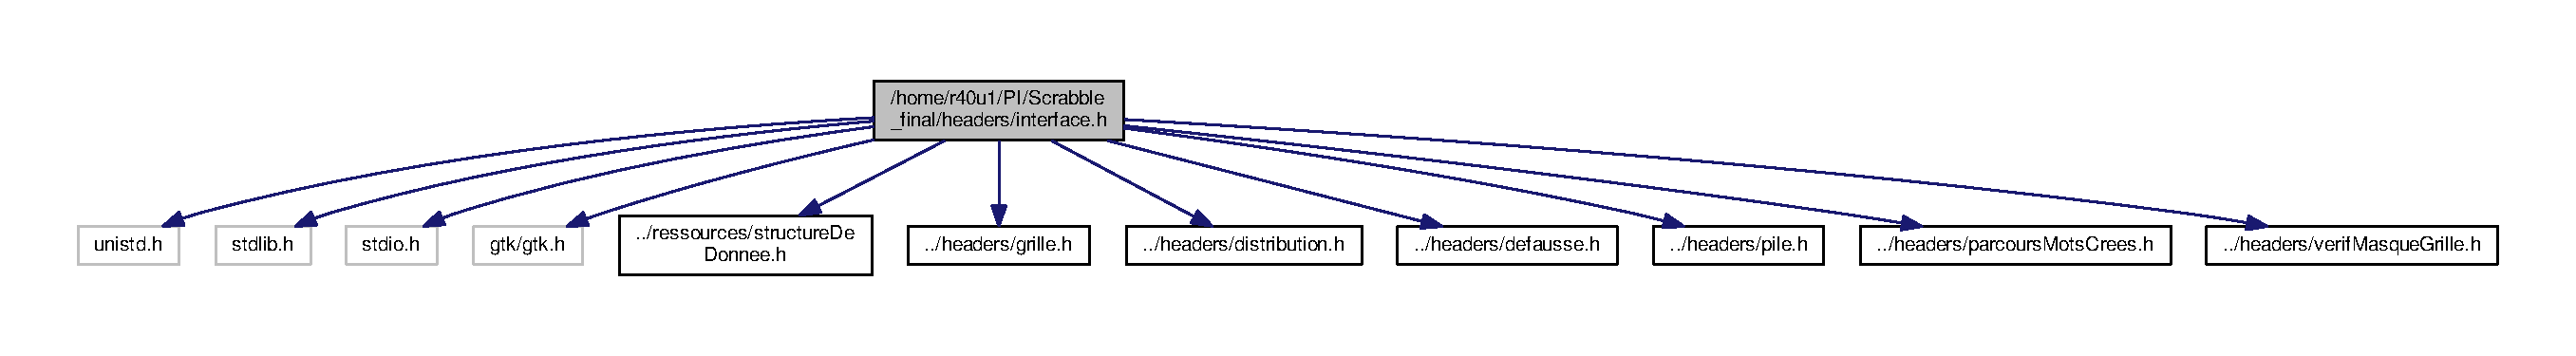
\includegraphics[width=350pt]{interface_8h__incl}
\end{center}
\end{figure}
This graph shows which files directly or indirectly include this file\-:\nopagebreak
\begin{figure}[H]
\begin{center}
\leavevmode
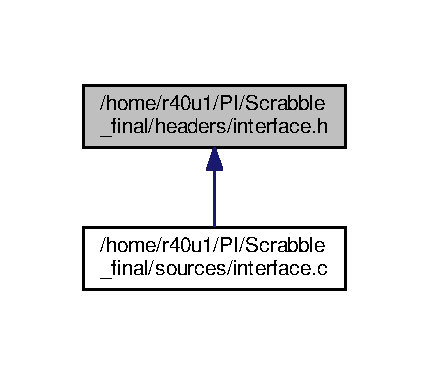
\includegraphics[width=206pt]{interface_8h__dep__incl}
\end{center}
\end{figure}
\subsection*{Data Structures}
\begin{DoxyCompactItemize}
\item 
struct \hyperlink{struct_image_cliquable}{Image\-Cliquable}
\end{DoxyCompactItemize}
\subsection*{Functions}
\begin{DoxyCompactItemize}
\item 
void \hyperlink{interface_8h_a526a8d1aec28b7ccca94fa2e02e4bd18}{choisir\-Nb\-Joueurs} ()
\item 
void \hyperlink{interface_8h_af4f096a4430a03ce24dfc96254e3134e}{on\-Destroy} (Gtk\-Widget $\ast$p\-Widget, gpointer p\-Data)
\item 
void \hyperlink{interface_8h_ad1473b9c475bd38e7d7ce6eda149da20}{tout\-Fermer} (Gtk\-Widget $\ast$p\-Widget, gpointer p\-Data)
\item 
void \hyperlink{interface_8h_a55fa3c7ab3754e3c68c49530878826c7}{rejouer} (Gtk\-Widget $\ast$p\-Widget, gpointer p\-Data)
\item 
void \hyperlink{interface_8h_a552443357dbe94d4a81110d2e30e4a4f}{on\-Destroy2} (Gtk\-Widget $\ast$p\-Widget, gpointer p\-Data)
\item 
void \hyperlink{interface_8h_a1df764e57151185f121c3a1414f9eca5}{nouvelle\-Partie} (Gtk\-Widget $\ast$p\-Widget, gpointer p\-Nb\-Joueurs)
\item 
void \hyperlink{interface_8h_a082c9bde05896c4cf8fadc76da463195}{sauvegarde\-Grille\-Chevalets} (void)
\item 
void \hyperlink{interface_8h_acdb6a13364defbabd5dbcd17cf340d39}{afficher\-Chevalet\-Joueur} (Gtk\-Widget $\ast$p\-Widget, gpointer p\-Data)
\item 
void \hyperlink{interface_8h_a4a8146490f83c8dd3b12d15dba38a129}{selectionner\-Lettre\-Choisie} (Gtk\-Widget $\ast$p\-Lettre\-Choisie, gpointer p\-Data)
\item 
void \hyperlink{interface_8h_a88fc771243ae35fae85bc4744960c921}{deselectionner\-Lettre\-Choisie} (Gtk\-Widget $\ast$p\-Widget, gpointer p\-Data)
\item 
void \hyperlink{interface_8h_aaa1ae69ef2562f9e5a48304b6c053069}{poser\-Lettre\-Choisie} (Gtk\-Widget $\ast$p\-Widget, gpointer p\-Data)
\item 
void \hyperlink{interface_8h_a5e7ffbbfe6b5f3f20c1aa94110a42578}{annuler\-Mot} (Gtk\-Widget $\ast$p\-Widget, gpointer p\-Data)
\item 
void \hyperlink{interface_8h_a9a4135ad9f77ef9f5ef05c6f719ef263}{defausser} (Gtk\-Widget $\ast$p\-Widget, gpointer p\-Data)
\item 
void \hyperlink{interface_8h_aefa85ce077ba68d6466ff40ff003e254}{defausser\-Lettre\-Choisie} (Gtk\-Widget $\ast$p\-Widget, gpointer p\-Data)
\item 
void \hyperlink{interface_8h_a848f4a9c0d47cd36d11bf242a509da1e}{annuler\-Defausser\-Lettre\-Choisie} (Gtk\-Widget $\ast$p\-Widget, gpointer p\-Data)
\item 
void \hyperlink{interface_8h_ace2219ff27db9cc42bd2f8ef2a1c6927}{valider\-Pose} (Gtk\-Widget $\ast$p\-Widget, gpointer p\-Data)
\item 
void \hyperlink{interface_8h_a215247abde0f785768cb4fa6f20c28bd}{valider\-Defausse} (Gtk\-Widget $\ast$p\-Widget, gpointer p\-Data)
\item 
void \hyperlink{interface_8h_abee2513b14c65f04e77e2e5791738c28}{passer\-Tour} (Gtk\-Widget $\ast$p\-Widget, gpointer p\-Data)
\item 
void \hyperlink{interface_8h_a0574bb936d7d1b923cd671de7fe3d31b}{fin\-De\-Partie} ()
\item 
void \hyperlink{interface_8h_a3bdd3a4c0dcf80136881ac584ca28459}{mise\-A\-Jour\-Chevalet} (\hyperlink{struct_image_cliquable}{Image\-Cliquable} \hyperlink{interface_8c_afd3d322d8336128bbf6d36ec762661c2}{p\-Chevalet}\mbox{[}7\mbox{]}, \hyperlink{structure_de_donnee_8h_abde700801ddcd10c40bdf389ff5b1494}{Chevalet} chevalet\-Virtuel)
\item 
void \hyperlink{interface_8h_a826440afda3f0a2fc08db2811ed1e426}{mise\-A\-Jour\-Grille} (\hyperlink{struct_image_cliquable}{Image\-Cliquable} \hyperlink{interface_8c_a240d2f78bb7839f241f70e92912b8f87}{p\-Quadrillage}\mbox{[}15\mbox{]}\mbox{[}15\mbox{]}, \hyperlink{structure_de_donnee_8h_a4b19d9524b7f293ad87dd6bd9d121b25}{Grille} grille)
\item 
void \hyperlink{interface_8h_acbdd784a6aaf43ec09f8e3a91f8ffe31}{gtk\-\_\-imagecliquable\-\_\-new} (\hyperlink{struct_image_cliquable}{Image\-Cliquable} $\ast$p\-Image\-Cliquable)
\item 
void \hyperlink{interface_8h_a83bbc8a0fb1c878f689795c5d9bb9219}{gtk\-\_\-imagecliquable\-\_\-set\-\_\-image\-\_\-from\-\_\-file} (\hyperlink{struct_image_cliquable}{Image\-Cliquable} $\ast$p\-Image\-Cliquable, char $\ast$file)
\end{DoxyCompactItemize}


\subsection{Function Documentation}
\hypertarget{interface_8h_acdb6a13364defbabd5dbcd17cf340d39}{\index{interface.\-h@{interface.\-h}!afficher\-Chevalet\-Joueur@{afficher\-Chevalet\-Joueur}}
\index{afficher\-Chevalet\-Joueur@{afficher\-Chevalet\-Joueur}!interface.h@{interface.\-h}}
\subsubsection[{afficher\-Chevalet\-Joueur}]{\setlength{\rightskip}{0pt plus 5cm}void afficher\-Chevalet\-Joueur (
\begin{DoxyParamCaption}
\item[{Gtk\-Widget $\ast$}]{p\-Widget, }
\item[{gpointer}]{p\-Data}
\end{DoxyParamCaption}
)}}\label{interface_8h_acdb6a13364defbabd5dbcd17cf340d39}
Le joueur est pret, on cree et affiche son chevalet \-: on attend qu'il choisisse un lettre a poser ou qu'il choisisse de se defausser \hypertarget{interface_8h_a848f4a9c0d47cd36d11bf242a509da1e}{\index{interface.\-h@{interface.\-h}!annuler\-Defausser\-Lettre\-Choisie@{annuler\-Defausser\-Lettre\-Choisie}}
\index{annuler\-Defausser\-Lettre\-Choisie@{annuler\-Defausser\-Lettre\-Choisie}!interface.h@{interface.\-h}}
\subsubsection[{annuler\-Defausser\-Lettre\-Choisie}]{\setlength{\rightskip}{0pt plus 5cm}void annuler\-Defausser\-Lettre\-Choisie (
\begin{DoxyParamCaption}
\item[{Gtk\-Widget $\ast$}]{p\-Widget, }
\item[{gpointer}]{p\-Data}
\end{DoxyParamCaption}
)}}\label{interface_8h_a848f4a9c0d47cd36d11bf242a509da1e}
Le joueur ne veut plus defausser cette lettre \hypertarget{interface_8h_a5e7ffbbfe6b5f3f20c1aa94110a42578}{\index{interface.\-h@{interface.\-h}!annuler\-Mot@{annuler\-Mot}}
\index{annuler\-Mot@{annuler\-Mot}!interface.h@{interface.\-h}}
\subsubsection[{annuler\-Mot}]{\setlength{\rightskip}{0pt plus 5cm}void annuler\-Mot (
\begin{DoxyParamCaption}
\item[{Gtk\-Widget $\ast$}]{p\-Widget, }
\item[{gpointer}]{p\-Data}
\end{DoxyParamCaption}
)}}\label{interface_8h_a5e7ffbbfe6b5f3f20c1aa94110a42578}
En cours de depose, le joueur ne veut plus poser son mot \-: on retablit la grille et le chevalet aux valeurs sauvegardees \hypertarget{interface_8h_a526a8d1aec28b7ccca94fa2e02e4bd18}{\index{interface.\-h@{interface.\-h}!choisir\-Nb\-Joueurs@{choisir\-Nb\-Joueurs}}
\index{choisir\-Nb\-Joueurs@{choisir\-Nb\-Joueurs}!interface.h@{interface.\-h}}
\subsubsection[{choisir\-Nb\-Joueurs}]{\setlength{\rightskip}{0pt plus 5cm}void choisir\-Nb\-Joueurs (
\begin{DoxyParamCaption}
{}
\end{DoxyParamCaption}
)}}\label{interface_8h_a526a8d1aec28b7ccca94fa2e02e4bd18}
Affichage de la fenetre permettant de choisir combien de joueurs vont jouer \-: on attend le choix du joueur \hypertarget{interface_8h_a9a4135ad9f77ef9f5ef05c6f719ef263}{\index{interface.\-h@{interface.\-h}!defausser@{defausser}}
\index{defausser@{defausser}!interface.h@{interface.\-h}}
\subsubsection[{defausser}]{\setlength{\rightskip}{0pt plus 5cm}void defausser (
\begin{DoxyParamCaption}
\item[{Gtk\-Widget $\ast$}]{p\-Widget, }
\item[{gpointer}]{p\-Data}
\end{DoxyParamCaption}
)}}\label{interface_8h_a9a4135ad9f77ef9f5ef05c6f719ef263}
Le joueur souhaite se defausser d'un certain nombre de ses jetons \hypertarget{interface_8h_aefa85ce077ba68d6466ff40ff003e254}{\index{interface.\-h@{interface.\-h}!defausser\-Lettre\-Choisie@{defausser\-Lettre\-Choisie}}
\index{defausser\-Lettre\-Choisie@{defausser\-Lettre\-Choisie}!interface.h@{interface.\-h}}
\subsubsection[{defausser\-Lettre\-Choisie}]{\setlength{\rightskip}{0pt plus 5cm}void defausser\-Lettre\-Choisie (
\begin{DoxyParamCaption}
\item[{Gtk\-Widget $\ast$}]{p\-Widget, }
\item[{gpointer}]{p\-Data}
\end{DoxyParamCaption}
)}}\label{interface_8h_aefa85ce077ba68d6466ff40ff003e254}
Le joueur a choisit une lettre a defausser \hypertarget{interface_8h_a88fc771243ae35fae85bc4744960c921}{\index{interface.\-h@{interface.\-h}!deselectionner\-Lettre\-Choisie@{deselectionner\-Lettre\-Choisie}}
\index{deselectionner\-Lettre\-Choisie@{deselectionner\-Lettre\-Choisie}!interface.h@{interface.\-h}}
\subsubsection[{deselectionner\-Lettre\-Choisie}]{\setlength{\rightskip}{0pt plus 5cm}void deselectionner\-Lettre\-Choisie (
\begin{DoxyParamCaption}
\item[{Gtk\-Widget $\ast$}]{p\-Widget, }
\item[{gpointer}]{p\-Data}
\end{DoxyParamCaption}
)}}\label{interface_8h_a88fc771243ae35fae85bc4744960c921}
Le joueur ne veut plus poser cette lettre \-: on attend qu'il en choisisse une autre \hypertarget{interface_8h_a0574bb936d7d1b923cd671de7fe3d31b}{\index{interface.\-h@{interface.\-h}!fin\-De\-Partie@{fin\-De\-Partie}}
\index{fin\-De\-Partie@{fin\-De\-Partie}!interface.h@{interface.\-h}}
\subsubsection[{fin\-De\-Partie}]{\setlength{\rightskip}{0pt plus 5cm}void fin\-De\-Partie (
\begin{DoxyParamCaption}
{}
\end{DoxyParamCaption}
)}}\label{interface_8h_a0574bb936d7d1b923cd671de7fe3d31b}
Le fin de la partie a ete declenchee \-: on affiche dans une nouvelle fenetre le score ainsi que le numero du gagnant \hypertarget{interface_8h_acbdd784a6aaf43ec09f8e3a91f8ffe31}{\index{interface.\-h@{interface.\-h}!gtk\-\_\-imagecliquable\-\_\-new@{gtk\-\_\-imagecliquable\-\_\-new}}
\index{gtk\-\_\-imagecliquable\-\_\-new@{gtk\-\_\-imagecliquable\-\_\-new}!interface.h@{interface.\-h}}
\subsubsection[{gtk\-\_\-imagecliquable\-\_\-new}]{\setlength{\rightskip}{0pt plus 5cm}void gtk\-\_\-imagecliquable\-\_\-new (
\begin{DoxyParamCaption}
\item[{{\bf Image\-Cliquable} $\ast$}]{p\-Image\-Cliquable}
\end{DoxyParamCaption}
)}}\label{interface_8h_acbdd784a6aaf43ec09f8e3a91f8ffe31}
initialisation d'une image cliquable \hypertarget{interface_8h_a83bbc8a0fb1c878f689795c5d9bb9219}{\index{interface.\-h@{interface.\-h}!gtk\-\_\-imagecliquable\-\_\-set\-\_\-image\-\_\-from\-\_\-file@{gtk\-\_\-imagecliquable\-\_\-set\-\_\-image\-\_\-from\-\_\-file}}
\index{gtk\-\_\-imagecliquable\-\_\-set\-\_\-image\-\_\-from\-\_\-file@{gtk\-\_\-imagecliquable\-\_\-set\-\_\-image\-\_\-from\-\_\-file}!interface.h@{interface.\-h}}
\subsubsection[{gtk\-\_\-imagecliquable\-\_\-set\-\_\-image\-\_\-from\-\_\-file}]{\setlength{\rightskip}{0pt plus 5cm}void gtk\-\_\-imagecliquable\-\_\-set\-\_\-image\-\_\-from\-\_\-file (
\begin{DoxyParamCaption}
\item[{{\bf Image\-Cliquable} $\ast$}]{p\-Image\-Cliquable, }
\item[{char $\ast$}]{file}
\end{DoxyParamCaption}
)}}\label{interface_8h_a83bbc8a0fb1c878f689795c5d9bb9219}
charger une image dans l'imagecliquable \hypertarget{interface_8h_a3bdd3a4c0dcf80136881ac584ca28459}{\index{interface.\-h@{interface.\-h}!mise\-A\-Jour\-Chevalet@{mise\-A\-Jour\-Chevalet}}
\index{mise\-A\-Jour\-Chevalet@{mise\-A\-Jour\-Chevalet}!interface.h@{interface.\-h}}
\subsubsection[{mise\-A\-Jour\-Chevalet}]{\setlength{\rightskip}{0pt plus 5cm}void mise\-A\-Jour\-Chevalet (
\begin{DoxyParamCaption}
\item[{{\bf Image\-Cliquable}}]{p\-Chevalet\mbox{[}7\mbox{]}, }
\item[{{\bf Chevalet}}]{chevalet\-Virtuel}
\end{DoxyParamCaption}
)}}\label{interface_8h_a3bdd3a4c0dcf80136881ac584ca28459}
Mise a jour des textes affiches sur les boutons de l'interface graphique au niveau du chevalet affiche \hypertarget{interface_8h_a826440afda3f0a2fc08db2811ed1e426}{\index{interface.\-h@{interface.\-h}!mise\-A\-Jour\-Grille@{mise\-A\-Jour\-Grille}}
\index{mise\-A\-Jour\-Grille@{mise\-A\-Jour\-Grille}!interface.h@{interface.\-h}}
\subsubsection[{mise\-A\-Jour\-Grille}]{\setlength{\rightskip}{0pt plus 5cm}void mise\-A\-Jour\-Grille (
\begin{DoxyParamCaption}
\item[{{\bf Image\-Cliquable}}]{p\-Quadrillage\mbox{[}15\mbox{]}\mbox{[}15\mbox{]}, }
\item[{{\bf Grille}}]{grille}
\end{DoxyParamCaption}
)}}\label{interface_8h_a826440afda3f0a2fc08db2811ed1e426}
Mise a jour des textes affiches sur les boutons de l'interface graphique au niveau de la grille \hypertarget{interface_8h_a1df764e57151185f121c3a1414f9eca5}{\index{interface.\-h@{interface.\-h}!nouvelle\-Partie@{nouvelle\-Partie}}
\index{nouvelle\-Partie@{nouvelle\-Partie}!interface.h@{interface.\-h}}
\subsubsection[{nouvelle\-Partie}]{\setlength{\rightskip}{0pt plus 5cm}void nouvelle\-Partie (
\begin{DoxyParamCaption}
\item[{Gtk\-Widget $\ast$}]{p\-Widget, }
\item[{gpointer}]{p\-Nb\-Joueurs}
\end{DoxyParamCaption}
)}}\label{interface_8h_a1df764e57151185f121c3a1414f9eca5}
Demarrage d'une nouvelle partie \-: creation des fenetres, de tous les boutons. On attend que le 1er joueur soit pret a commencer \hypertarget{interface_8h_af4f096a4430a03ce24dfc96254e3134e}{\index{interface.\-h@{interface.\-h}!on\-Destroy@{on\-Destroy}}
\index{on\-Destroy@{on\-Destroy}!interface.h@{interface.\-h}}
\subsubsection[{on\-Destroy}]{\setlength{\rightskip}{0pt plus 5cm}void on\-Destroy (
\begin{DoxyParamCaption}
\item[{Gtk\-Widget $\ast$}]{p\-Widget, }
\item[{gpointer}]{p\-Data}
\end{DoxyParamCaption}
)}}\label{interface_8h_af4f096a4430a03ce24dfc96254e3134e}
Fermeture de la fenetre en cours \hypertarget{interface_8h_a552443357dbe94d4a81110d2e30e4a4f}{\index{interface.\-h@{interface.\-h}!on\-Destroy2@{on\-Destroy2}}
\index{on\-Destroy2@{on\-Destroy2}!interface.h@{interface.\-h}}
\subsubsection[{on\-Destroy2}]{\setlength{\rightskip}{0pt plus 5cm}void on\-Destroy2 (
\begin{DoxyParamCaption}
\item[{Gtk\-Widget $\ast$}]{p\-Widget, }
\item[{gpointer}]{p\-Data}
\end{DoxyParamCaption}
)}}\label{interface_8h_a552443357dbe94d4a81110d2e30e4a4f}
Fermeture de la fenetre de jeu et retour au choix du nombre de joueur \hypertarget{interface_8h_abee2513b14c65f04e77e2e5791738c28}{\index{interface.\-h@{interface.\-h}!passer\-Tour@{passer\-Tour}}
\index{passer\-Tour@{passer\-Tour}!interface.h@{interface.\-h}}
\subsubsection[{passer\-Tour}]{\setlength{\rightskip}{0pt plus 5cm}void passer\-Tour (
\begin{DoxyParamCaption}
\item[{Gtk\-Widget $\ast$}]{p\-Widget, }
\item[{gpointer}]{p\-Data}
\end{DoxyParamCaption}
)}}\label{interface_8h_abee2513b14c65f04e77e2e5791738c28}
Le joueur ne peut rien faire, il passe son tour, on passe au joueur suivant \hypertarget{interface_8h_aaa1ae69ef2562f9e5a48304b6c053069}{\index{interface.\-h@{interface.\-h}!poser\-Lettre\-Choisie@{poser\-Lettre\-Choisie}}
\index{poser\-Lettre\-Choisie@{poser\-Lettre\-Choisie}!interface.h@{interface.\-h}}
\subsubsection[{poser\-Lettre\-Choisie}]{\setlength{\rightskip}{0pt plus 5cm}void poser\-Lettre\-Choisie (
\begin{DoxyParamCaption}
\item[{Gtk\-Widget $\ast$}]{p\-Widget, }
\item[{gpointer}]{p\-Data}
\end{DoxyParamCaption}
)}}\label{interface_8h_aaa1ae69ef2562f9e5a48304b6c053069}
Le joueur a choisi la case sur laquelle poser la lettre desiree \-: on attend qu'il en choisisse une autre ou qu'il valide son mot (ou qu'il annule) \hypertarget{interface_8h_a55fa3c7ab3754e3c68c49530878826c7}{\index{interface.\-h@{interface.\-h}!rejouer@{rejouer}}
\index{rejouer@{rejouer}!interface.h@{interface.\-h}}
\subsubsection[{rejouer}]{\setlength{\rightskip}{0pt plus 5cm}void rejouer (
\begin{DoxyParamCaption}
\item[{Gtk\-Widget $\ast$}]{p\-Widget, }
\item[{gpointer}]{p\-Data}
\end{DoxyParamCaption}
)}}\label{interface_8h_a55fa3c7ab3754e3c68c49530878826c7}
Fermeture de toutes les fenetres + Reouverture de celle du choix du nombre de joueur \hypertarget{interface_8h_a082c9bde05896c4cf8fadc76da463195}{\index{interface.\-h@{interface.\-h}!sauvegarde\-Grille\-Chevalets@{sauvegarde\-Grille\-Chevalets}}
\index{sauvegarde\-Grille\-Chevalets@{sauvegarde\-Grille\-Chevalets}!interface.h@{interface.\-h}}
\subsubsection[{sauvegarde\-Grille\-Chevalets}]{\setlength{\rightskip}{0pt plus 5cm}void sauvegarde\-Grille\-Chevalets (
\begin{DoxyParamCaption}
\item[{void}]{}
\end{DoxyParamCaption}
)}}\label{interface_8h_a082c9bde05896c4cf8fadc76da463195}
On sauvegarde la grille et le chevalet au cas ou le joueur voudrait annuler son depot de lettre (ou si son mot n'existe pas etc) \hypertarget{interface_8h_a4a8146490f83c8dd3b12d15dba38a129}{\index{interface.\-h@{interface.\-h}!selectionner\-Lettre\-Choisie@{selectionner\-Lettre\-Choisie}}
\index{selectionner\-Lettre\-Choisie@{selectionner\-Lettre\-Choisie}!interface.h@{interface.\-h}}
\subsubsection[{selectionner\-Lettre\-Choisie}]{\setlength{\rightskip}{0pt plus 5cm}void selectionner\-Lettre\-Choisie (
\begin{DoxyParamCaption}
\item[{Gtk\-Widget $\ast$}]{p\-Lettre\-Choisie, }
\item[{gpointer}]{p\-Data}
\end{DoxyParamCaption}
)}}\label{interface_8h_a4a8146490f83c8dd3b12d15dba38a129}
Le joueur a clique sur la lettre qu'il veut poser \-: on attend qu'il choisisse ou la poser (ou qu'il annule) \hypertarget{interface_8h_ad1473b9c475bd38e7d7ce6eda149da20}{\index{interface.\-h@{interface.\-h}!tout\-Fermer@{tout\-Fermer}}
\index{tout\-Fermer@{tout\-Fermer}!interface.h@{interface.\-h}}
\subsubsection[{tout\-Fermer}]{\setlength{\rightskip}{0pt plus 5cm}void tout\-Fermer (
\begin{DoxyParamCaption}
\item[{Gtk\-Widget $\ast$}]{p\-Widget, }
\item[{gpointer}]{p\-Data}
\end{DoxyParamCaption}
)}}\label{interface_8h_ad1473b9c475bd38e7d7ce6eda149da20}
Fermeture de toutes les fenetres \hypertarget{interface_8h_a215247abde0f785768cb4fa6f20c28bd}{\index{interface.\-h@{interface.\-h}!valider\-Defausse@{valider\-Defausse}}
\index{valider\-Defausse@{valider\-Defausse}!interface.h@{interface.\-h}}
\subsubsection[{valider\-Defausse}]{\setlength{\rightskip}{0pt plus 5cm}void valider\-Defausse (
\begin{DoxyParamCaption}
\item[{Gtk\-Widget $\ast$}]{p\-Widget, }
\item[{gpointer}]{p\-Data}
\end{DoxyParamCaption}
)}}\label{interface_8h_a215247abde0f785768cb4fa6f20c28bd}
Le joueur valide son choix de lettres a defausser, on lui en distribue d'autres et on passe au joueur suivant \hypertarget{interface_8h_ace2219ff27db9cc42bd2f8ef2a1c6927}{\index{interface.\-h@{interface.\-h}!valider\-Pose@{valider\-Pose}}
\index{valider\-Pose@{valider\-Pose}!interface.h@{interface.\-h}}
\subsubsection[{valider\-Pose}]{\setlength{\rightskip}{0pt plus 5cm}void valider\-Pose (
\begin{DoxyParamCaption}
\item[{Gtk\-Widget $\ast$}]{p\-Widget, }
\item[{gpointer}]{p\-Data}
\end{DoxyParamCaption}
)}}\label{interface_8h_ace2219ff27db9cc42bd2f8ef2a1c6927}
Le joueur valide son mot \-: on verifie que tout est bon sinon on restaure au chevalet et a la grille sauvegardee 
\hypertarget{parcours_mots_crees_8h}{\section{/home/r40u1/\-P\-I/\-Scrabble\-\_\-final/headers/parcours\-Mots\-Crees.h File Reference}
\label{parcours_mots_crees_8h}\index{/home/r40u1/\-P\-I/\-Scrabble\-\_\-final/headers/parcours\-Mots\-Crees.\-h@{/home/r40u1/\-P\-I/\-Scrabble\-\_\-final/headers/parcours\-Mots\-Crees.\-h}}
}
This graph shows which files directly or indirectly include this file\-:\nopagebreak
\begin{figure}[H]
\begin{center}
\leavevmode
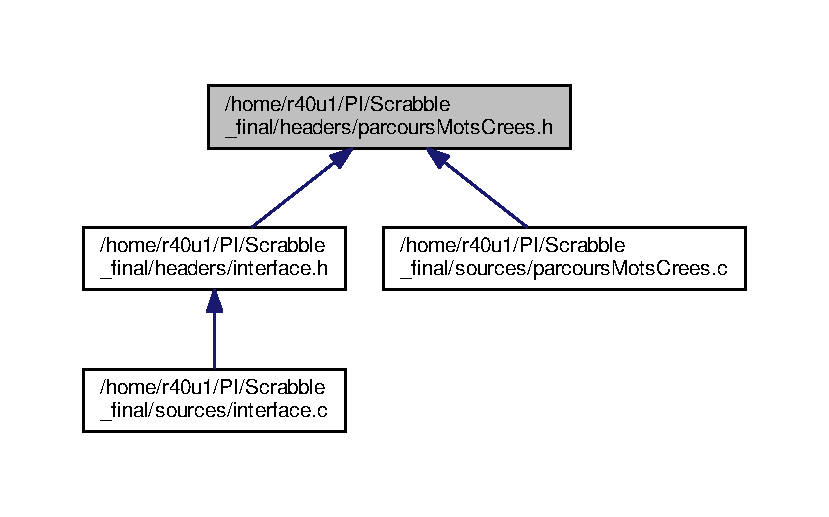
\includegraphics[width=350pt]{parcours_mots_crees_8h__dep__incl}
\end{center}
\end{figure}
\subsection*{Functions}
\begin{DoxyCompactItemize}
\item 
void \hyperlink{parcours_mots_crees_8h_aa81d9b49470738820a7a926be0641490}{calculer\-Score} (int i1, int j1, int i2, int j2, \hyperlink{structure_de_donnee_8h_a4b19d9524b7f293ad87dd6bd9d121b25}{Grille} grille, \hyperlink{structure_de_donnee_8h_a426c0d223e7dc6b87d723c4c0c0e1f58}{Booleen} $\ast$p\-Existence, int $\ast$p\-Score)
\item 
void \hyperlink{parcours_mots_crees_8h_a4be650a0062b7277a7d2980abb5cffe3}{parcours\-Des\-Mots\-Crees} (\hyperlink{structure_de_donnee_8h_a4b19d9524b7f293ad87dd6bd9d121b25}{Grille} grille, char sens, int l0, int c0, int n, \hyperlink{structure_de_donnee_8h_a426c0d223e7dc6b87d723c4c0c0e1f58}{Booleen} $\ast$p\-Existence, int $\ast$p\-Score, int \hyperlink{interface_8c_ad5bfefafa3d248972817c0259efa829d}{masque\-Grille}\mbox{[}15\mbox{]}\mbox{[}15\mbox{]}, int $\ast$p\-Touche, char \hyperlink{interface_8c_ad3e01a56d5cdbd89e97b9b9346bc1a54}{message}\mbox{[}200\mbox{]})
\end{DoxyCompactItemize}


\subsection{Function Documentation}
\hypertarget{parcours_mots_crees_8h_aa81d9b49470738820a7a926be0641490}{\index{parcours\-Mots\-Crees.\-h@{parcours\-Mots\-Crees.\-h}!calculer\-Score@{calculer\-Score}}
\index{calculer\-Score@{calculer\-Score}!parcoursMotsCrees.h@{parcours\-Mots\-Crees.\-h}}
\subsubsection[{calculer\-Score}]{\setlength{\rightskip}{0pt plus 5cm}void calculer\-Score (
\begin{DoxyParamCaption}
\item[{int}]{i1, }
\item[{int}]{j1, }
\item[{int}]{i2, }
\item[{int}]{j2, }
\item[{{\bf Grille}}]{grille, }
\item[{{\bf Booleen} $\ast$}]{p\-Existence, }
\item[{int $\ast$}]{p\-Score}
\end{DoxyParamCaption}
)}}\label{parcours_mots_crees_8h_aa81d9b49470738820a7a926be0641490}
à partir des coordonnées d'une suite de lettre, détermine si le mot existe et, si tel est le cas, le nombre de point qu'il rapporte \hypertarget{parcours_mots_crees_8h_a4be650a0062b7277a7d2980abb5cffe3}{\index{parcours\-Mots\-Crees.\-h@{parcours\-Mots\-Crees.\-h}!parcours\-Des\-Mots\-Crees@{parcours\-Des\-Mots\-Crees}}
\index{parcours\-Des\-Mots\-Crees@{parcours\-Des\-Mots\-Crees}!parcoursMotsCrees.h@{parcours\-Mots\-Crees.\-h}}
\subsubsection[{parcours\-Des\-Mots\-Crees}]{\setlength{\rightskip}{0pt plus 5cm}void parcours\-Des\-Mots\-Crees (
\begin{DoxyParamCaption}
\item[{{\bf Grille}}]{grille, }
\item[{char}]{sens, }
\item[{int}]{l0, }
\item[{int}]{c0, }
\item[{int}]{n, }
\item[{{\bf Booleen} $\ast$}]{p\-Tour\-Valide, }
\item[{int $\ast$}]{p\-Score\-Tour, }
\item[{int}]{masque\-Grille\mbox{[}15\mbox{]}\mbox{[}15\mbox{]}, }
\item[{int $\ast$}]{p\-Touche, }
\item[{char}]{message\mbox{[}200\mbox{]}}
\end{DoxyParamCaption}
)}}\label{parcours_mots_crees_8h_a4be650a0062b7277a7d2980abb5cffe3}
recherche tous les mots créés par la dépose des lettres du jouer + détermination de la validité du tour + le cas échéant, du score remporté 
\hypertarget{pile_8h}{\section{/home/r40u1/\-P\-I/\-Scrabble\-\_\-final/headers/pile.h File Reference}
\label{pile_8h}\index{/home/r40u1/\-P\-I/\-Scrabble\-\_\-final/headers/pile.\-h@{/home/r40u1/\-P\-I/\-Scrabble\-\_\-final/headers/pile.\-h}}
}
This graph shows which files directly or indirectly include this file\-:\nopagebreak
\begin{figure}[H]
\begin{center}
\leavevmode
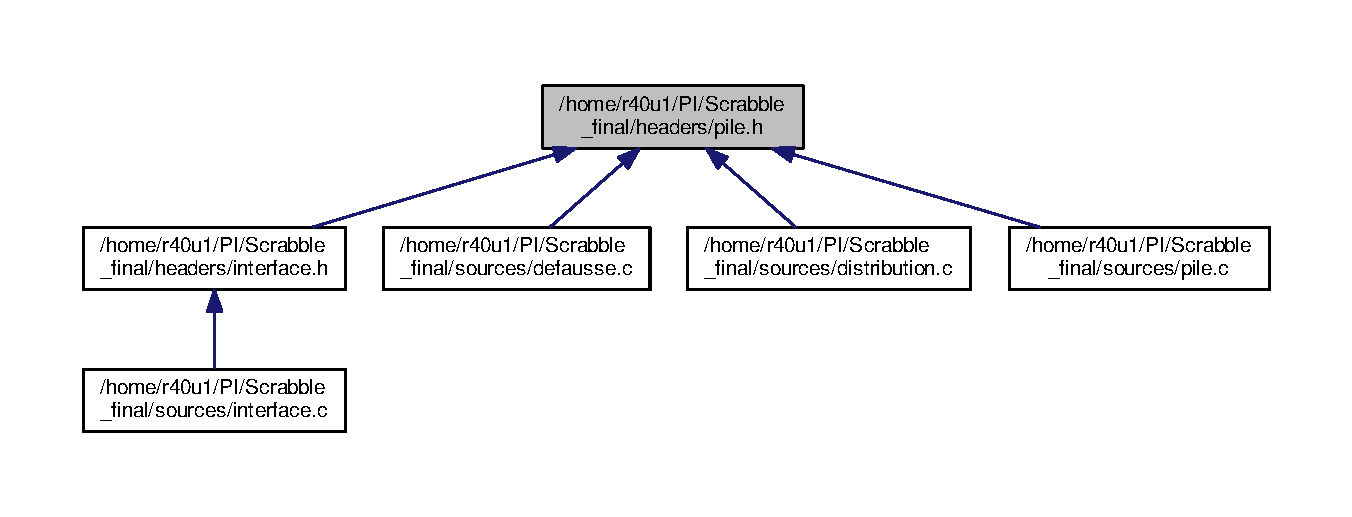
\includegraphics[width=350pt]{pile_8h__dep__incl}
\end{center}
\end{figure}
\subsection*{Functions}
\begin{DoxyCompactItemize}
\item 
\hyperlink{structure_de_donnee_8h_aeb2e4c1daa2de38a0efbf9ab87674140}{Pile} \hyperlink{pile_8h_ad08f6ed24f392bbe68d376207a77c22a}{nouvelle\-Pile} (void)
\item 
void \hyperlink{pile_8h_a4303633aa3fcd700657b6d76a58a9e40}{empiler} (\hyperlink{structure_de_donnee_8h_aeb2e4c1daa2de38a0efbf9ab87674140}{Pile} $\ast$ppile, \hyperlink{struct_jeton}{Jeton} jet)
\item 
\hyperlink{struct_jeton}{Jeton} \hyperlink{pile_8h_a43c3894da262ce42a5ddcafb39e0bdd6}{depiler} (\hyperlink{structure_de_donnee_8h_aeb2e4c1daa2de38a0efbf9ab87674140}{Pile} $\ast$ppile)
\end{DoxyCompactItemize}


\subsection{Function Documentation}
\hypertarget{pile_8h_a43c3894da262ce42a5ddcafb39e0bdd6}{\index{pile.\-h@{pile.\-h}!depiler@{depiler}}
\index{depiler@{depiler}!pile.h@{pile.\-h}}
\subsubsection[{depiler}]{\setlength{\rightskip}{0pt plus 5cm}{\bf Jeton} depiler (
\begin{DoxyParamCaption}
\item[{{\bf Pile} $\ast$}]{ppile}
\end{DoxyParamCaption}
)}}\label{pile_8h_a43c3894da262ce42a5ddcafb39e0bdd6}
\hypertarget{pile_8h_a4303633aa3fcd700657b6d76a58a9e40}{\index{pile.\-h@{pile.\-h}!empiler@{empiler}}
\index{empiler@{empiler}!pile.h@{pile.\-h}}
\subsubsection[{empiler}]{\setlength{\rightskip}{0pt plus 5cm}void empiler (
\begin{DoxyParamCaption}
\item[{{\bf Pile} $\ast$}]{ppile, }
\item[{{\bf Jeton}}]{jet}
\end{DoxyParamCaption}
)}}\label{pile_8h_a4303633aa3fcd700657b6d76a58a9e40}
\hypertarget{pile_8h_ad08f6ed24f392bbe68d376207a77c22a}{\index{pile.\-h@{pile.\-h}!nouvelle\-Pile@{nouvelle\-Pile}}
\index{nouvelle\-Pile@{nouvelle\-Pile}!pile.h@{pile.\-h}}
\subsubsection[{nouvelle\-Pile}]{\setlength{\rightskip}{0pt plus 5cm}{\bf Pile} nouvelle\-Pile (
\begin{DoxyParamCaption}
\item[{void}]{}
\end{DoxyParamCaption}
)}}\label{pile_8h_ad08f6ed24f392bbe68d376207a77c22a}

\hypertarget{verif_masque_grille_8h}{\section{/home/r40u1/\-P\-I/\-Scrabble\-\_\-final/headers/verif\-Masque\-Grille.h File Reference}
\label{verif_masque_grille_8h}\index{/home/r40u1/\-P\-I/\-Scrabble\-\_\-final/headers/verif\-Masque\-Grille.\-h@{/home/r40u1/\-P\-I/\-Scrabble\-\_\-final/headers/verif\-Masque\-Grille.\-h}}
}
This graph shows which files directly or indirectly include this file\-:\nopagebreak
\begin{figure}[H]
\begin{center}
\leavevmode
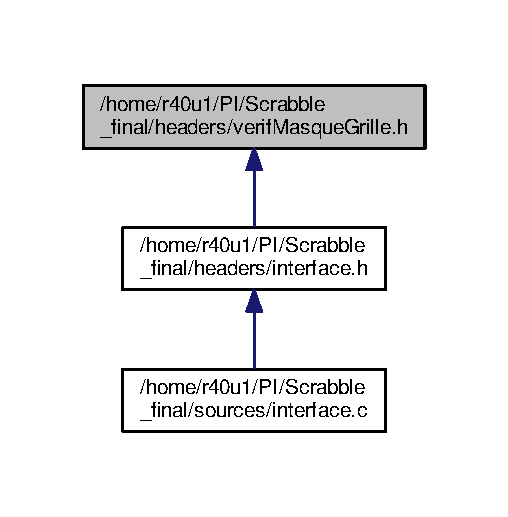
\includegraphics[width=244pt]{verif_masque_grille_8h__dep__incl}
\end{center}
\end{figure}
\subsection*{Functions}
\begin{DoxyCompactItemize}
\item 
int \hyperlink{verif_masque_grille_8h_ac29290023806fc031a3c481e48755ea7}{verif\-Masque\-Grille} (\hyperlink{structure_de_donnee_8h_a4b19d9524b7f293ad87dd6bd9d121b25}{Grille} grille, char $\ast$p\-Sens, int $\ast$p\-L0, int $\ast$p\-C0, int $\ast$p\-N, int \hyperlink{interface_8c_ad5bfefafa3d248972817c0259efa829d}{masque\-Grille}\mbox{[}15\mbox{]}\mbox{[}15\mbox{]}, int $\ast$touche, char \hyperlink{interface_8c_ad3e01a56d5cdbd89e97b9b9346bc1a54}{message}\mbox{[}200\mbox{]})
\end{DoxyCompactItemize}


\subsection{Function Documentation}
\hypertarget{verif_masque_grille_8h_ac29290023806fc031a3c481e48755ea7}{\index{verif\-Masque\-Grille.\-h@{verif\-Masque\-Grille.\-h}!verif\-Masque\-Grille@{verif\-Masque\-Grille}}
\index{verif\-Masque\-Grille@{verif\-Masque\-Grille}!verifMasqueGrille.h@{verif\-Masque\-Grille.\-h}}
\subsubsection[{verif\-Masque\-Grille}]{\setlength{\rightskip}{0pt plus 5cm}int verif\-Masque\-Grille (
\begin{DoxyParamCaption}
\item[{{\bf Grille}}]{grille, }
\item[{char $\ast$}]{p\-Sens, }
\item[{int $\ast$}]{p\-L0, }
\item[{int $\ast$}]{p\-C0, }
\item[{int $\ast$}]{p\-N, }
\item[{int}]{masque\-Grille\mbox{[}15\mbox{]}\mbox{[}15\mbox{]}, }
\item[{int $\ast$}]{p\-Touche, }
\item[{char}]{message\mbox{[}200\mbox{]}}
\end{DoxyParamCaption}
)}}\label{verif_masque_grille_8h_ac29290023806fc031a3c481e48755ea7}
Verifie grossièrement si l'emplacement des lettres posees n'est pas incoherent 
\hypertarget{structure_de_donnee_8h}{\section{structure\-De\-Donnee.\-h File Reference}
\label{structure_de_donnee_8h}\index{structure\-De\-Donnee.\-h@{structure\-De\-Donnee.\-h}}
}
This graph shows which files directly or indirectly include this file\-:\nopagebreak
\begin{figure}[H]
\begin{center}
\leavevmode
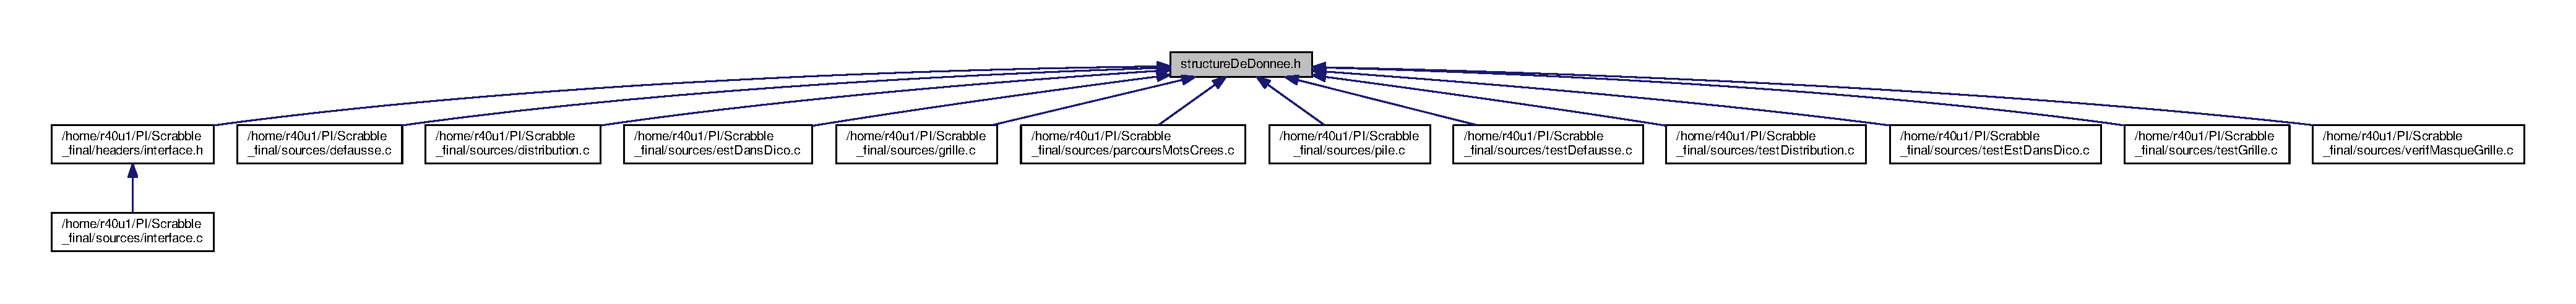
\includegraphics[width=350pt]{structure_de_donnee_8h__dep__incl}
\end{center}
\end{figure}
\subsection*{Data Structures}
\begin{DoxyCompactItemize}
\item 
struct \hyperlink{struct_jeton}{Jeton}
\item 
struct \hyperlink{struct_case}{Case}
\item 
struct \hyperlink{structelement}{element}
\end{DoxyCompactItemize}
\subsection*{Macros}
\begin{DoxyCompactItemize}
\item 
\#define \hyperlink{structure_de_donnee_8h_a71e2e07f0ea54740cb5421e00e77a979}{N\-O\-M\-B\-R\-E\-D\-E\-J\-E\-T\-O\-N}~102
\item 
\#define \hyperlink{structure_de_donnee_8h_a327caefea71c0d68121c20977dcda229}{C\-O\-T\-E\-G\-R\-I\-L\-L\-E}~15
\end{DoxyCompactItemize}
\subsection*{Typedefs}
\begin{DoxyCompactItemize}
\item 
typedef struct \hyperlink{struct_jeton}{Jeton} \hyperlink{structure_de_donnee_8h_abe5c8afd7d6a918e823c4464e8718af2}{Jeton}
\item 
typedef struct \hyperlink{structelement}{element} \hyperlink{structure_de_donnee_8h_a19e5efbe1d06b9433421e5035afbe873}{Element}
\item 
typedef \hyperlink{structure_de_donnee_8h_a19e5efbe1d06b9433421e5035afbe873}{Element} $\ast$ \hyperlink{structure_de_donnee_8h_aeb2e4c1daa2de38a0efbf9ab87674140}{Pile}
\item 
typedef \hyperlink{struct_jeton}{Jeton} \hyperlink{structure_de_donnee_8h_abde700801ddcd10c40bdf389ff5b1494}{Chevalet} \mbox{[}7\mbox{]}
\item 
typedef \hyperlink{struct_case}{Case} \hyperlink{structure_de_donnee_8h_a4b19d9524b7f293ad87dd6bd9d121b25}{Grille} \mbox{[}\hyperlink{structure_de_donnee_8h_a327caefea71c0d68121c20977dcda229}{C\-O\-T\-E\-G\-R\-I\-L\-L\-E}\mbox{]}\mbox{[}\hyperlink{structure_de_donnee_8h_a327caefea71c0d68121c20977dcda229}{C\-O\-T\-E\-G\-R\-I\-L\-L\-E}\mbox{]}
\end{DoxyCompactItemize}
\subsection*{Enumerations}
\begin{DoxyCompactItemize}
\item 
enum \hyperlink{structure_de_donnee_8h_a426c0d223e7dc6b87d723c4c0c0e1f58}{Booleen} \{ \hyperlink{structure_de_donnee_8h_a426c0d223e7dc6b87d723c4c0c0e1f58a1bb75a30f93b418be2d44aa0eafe9be3}{F\-A\-U\-X}, 
\hyperlink{structure_de_donnee_8h_a426c0d223e7dc6b87d723c4c0c0e1f58a763723ffe7a348ad0f5c1b58a331b523}{V\-R\-A\-I}
 \}
\end{DoxyCompactItemize}


\subsection{Macro Definition Documentation}
\hypertarget{structure_de_donnee_8h_a327caefea71c0d68121c20977dcda229}{\index{structure\-De\-Donnee.\-h@{structure\-De\-Donnee.\-h}!C\-O\-T\-E\-G\-R\-I\-L\-L\-E@{C\-O\-T\-E\-G\-R\-I\-L\-L\-E}}
\index{C\-O\-T\-E\-G\-R\-I\-L\-L\-E@{C\-O\-T\-E\-G\-R\-I\-L\-L\-E}!structureDeDonnee.h@{structure\-De\-Donnee.\-h}}
\subsubsection[{C\-O\-T\-E\-G\-R\-I\-L\-L\-E}]{\setlength{\rightskip}{0pt plus 5cm}\#define C\-O\-T\-E\-G\-R\-I\-L\-L\-E~15}}\label{structure_de_donnee_8h_a327caefea71c0d68121c20977dcda229}
\hypertarget{structure_de_donnee_8h_a71e2e07f0ea54740cb5421e00e77a979}{\index{structure\-De\-Donnee.\-h@{structure\-De\-Donnee.\-h}!N\-O\-M\-B\-R\-E\-D\-E\-J\-E\-T\-O\-N@{N\-O\-M\-B\-R\-E\-D\-E\-J\-E\-T\-O\-N}}
\index{N\-O\-M\-B\-R\-E\-D\-E\-J\-E\-T\-O\-N@{N\-O\-M\-B\-R\-E\-D\-E\-J\-E\-T\-O\-N}!structureDeDonnee.h@{structure\-De\-Donnee.\-h}}
\subsubsection[{N\-O\-M\-B\-R\-E\-D\-E\-J\-E\-T\-O\-N}]{\setlength{\rightskip}{0pt plus 5cm}\#define N\-O\-M\-B\-R\-E\-D\-E\-J\-E\-T\-O\-N~102}}\label{structure_de_donnee_8h_a71e2e07f0ea54740cb5421e00e77a979}


\subsection{Typedef Documentation}
\hypertarget{structure_de_donnee_8h_abde700801ddcd10c40bdf389ff5b1494}{\index{structure\-De\-Donnee.\-h@{structure\-De\-Donnee.\-h}!Chevalet@{Chevalet}}
\index{Chevalet@{Chevalet}!structureDeDonnee.h@{structure\-De\-Donnee.\-h}}
\subsubsection[{Chevalet}]{\setlength{\rightskip}{0pt plus 5cm}typedef {\bf Jeton} Chevalet\mbox{[}7\mbox{]}}}\label{structure_de_donnee_8h_abde700801ddcd10c40bdf389ff5b1494}
\hypertarget{structure_de_donnee_8h_a19e5efbe1d06b9433421e5035afbe873}{\index{structure\-De\-Donnee.\-h@{structure\-De\-Donnee.\-h}!Element@{Element}}
\index{Element@{Element}!structureDeDonnee.h@{structure\-De\-Donnee.\-h}}
\subsubsection[{Element}]{\setlength{\rightskip}{0pt plus 5cm}typedef struct {\bf element}  {\bf Element}}}\label{structure_de_donnee_8h_a19e5efbe1d06b9433421e5035afbe873}
\hypertarget{structure_de_donnee_8h_a4b19d9524b7f293ad87dd6bd9d121b25}{\index{structure\-De\-Donnee.\-h@{structure\-De\-Donnee.\-h}!Grille@{Grille}}
\index{Grille@{Grille}!structureDeDonnee.h@{structure\-De\-Donnee.\-h}}
\subsubsection[{Grille}]{\setlength{\rightskip}{0pt plus 5cm}typedef {\bf Case} Grille\mbox{[}{\bf C\-O\-T\-E\-G\-R\-I\-L\-L\-E}\mbox{]}\mbox{[}{\bf C\-O\-T\-E\-G\-R\-I\-L\-L\-E}\mbox{]}}}\label{structure_de_donnee_8h_a4b19d9524b7f293ad87dd6bd9d121b25}
\hypertarget{structure_de_donnee_8h_abe5c8afd7d6a918e823c4464e8718af2}{\index{structure\-De\-Donnee.\-h@{structure\-De\-Donnee.\-h}!Jeton@{Jeton}}
\index{Jeton@{Jeton}!structureDeDonnee.h@{structure\-De\-Donnee.\-h}}
\subsubsection[{Jeton}]{\setlength{\rightskip}{0pt plus 5cm}typedef struct {\bf Jeton}  {\bf Jeton}}}\label{structure_de_donnee_8h_abe5c8afd7d6a918e823c4464e8718af2}
\hypertarget{structure_de_donnee_8h_aeb2e4c1daa2de38a0efbf9ab87674140}{\index{structure\-De\-Donnee.\-h@{structure\-De\-Donnee.\-h}!Pile@{Pile}}
\index{Pile@{Pile}!structureDeDonnee.h@{structure\-De\-Donnee.\-h}}
\subsubsection[{Pile}]{\setlength{\rightskip}{0pt plus 5cm}typedef {\bf Element}$\ast$ {\bf Pile}}}\label{structure_de_donnee_8h_aeb2e4c1daa2de38a0efbf9ab87674140}


\subsection{Enumeration Type Documentation}
\hypertarget{structure_de_donnee_8h_a426c0d223e7dc6b87d723c4c0c0e1f58}{\index{structure\-De\-Donnee.\-h@{structure\-De\-Donnee.\-h}!Booleen@{Booleen}}
\index{Booleen@{Booleen}!structureDeDonnee.h@{structure\-De\-Donnee.\-h}}
\subsubsection[{Booleen}]{\setlength{\rightskip}{0pt plus 5cm}enum {\bf Booleen}}}\label{structure_de_donnee_8h_a426c0d223e7dc6b87d723c4c0c0e1f58}
\begin{Desc}
\item[Enumerator]\par
\begin{description}
\index{F\-A\-U\-X@{F\-A\-U\-X}!structure\-De\-Donnee.\-h@{structure\-De\-Donnee.\-h}}\index{structure\-De\-Donnee.\-h@{structure\-De\-Donnee.\-h}!F\-A\-U\-X@{F\-A\-U\-X}}\item[{\em 
\hypertarget{structure_de_donnee_8h_a426c0d223e7dc6b87d723c4c0c0e1f58a1bb75a30f93b418be2d44aa0eafe9be3}{F\-A\-U\-X}\label{structure_de_donnee_8h_a426c0d223e7dc6b87d723c4c0c0e1f58a1bb75a30f93b418be2d44aa0eafe9be3}
}]\index{V\-R\-A\-I@{V\-R\-A\-I}!structure\-De\-Donnee.\-h@{structure\-De\-Donnee.\-h}}\index{structure\-De\-Donnee.\-h@{structure\-De\-Donnee.\-h}!V\-R\-A\-I@{V\-R\-A\-I}}\item[{\em 
\hypertarget{structure_de_donnee_8h_a426c0d223e7dc6b87d723c4c0c0e1f58a763723ffe7a348ad0f5c1b58a331b523}{V\-R\-A\-I}\label{structure_de_donnee_8h_a426c0d223e7dc6b87d723c4c0c0e1f58a763723ffe7a348ad0f5c1b58a331b523}
}]\end{description}
\end{Desc}

\hypertarget{defausse_8c}{\section{/home/r40u1/\-P\-I/\-Scrabble\-\_\-final/sources/defausse.c File Reference}
\label{defausse_8c}\index{/home/r40u1/\-P\-I/\-Scrabble\-\_\-final/sources/defausse.\-c@{/home/r40u1/\-P\-I/\-Scrabble\-\_\-final/sources/defausse.\-c}}
}
{\ttfamily \#include $<$stdlib.\-h$>$}\\*
{\ttfamily \#include $<$stdio.\-h$>$}\\*
{\ttfamily \#include \char`\"{}../ressources/structure\-De\-Donnee.\-h\char`\"{}}\\*
{\ttfamily \#include \char`\"{}../headers/defausse.\-h\char`\"{}}\\*
{\ttfamily \#include \char`\"{}../headers/pile.\-h\char`\"{}}\\*
{\ttfamily \#include \char`\"{}../headers/distribution.\-h\char`\"{}}\\*
Include dependency graph for defausse.\-c\-:\nopagebreak
\begin{figure}[H]
\begin{center}
\leavevmode
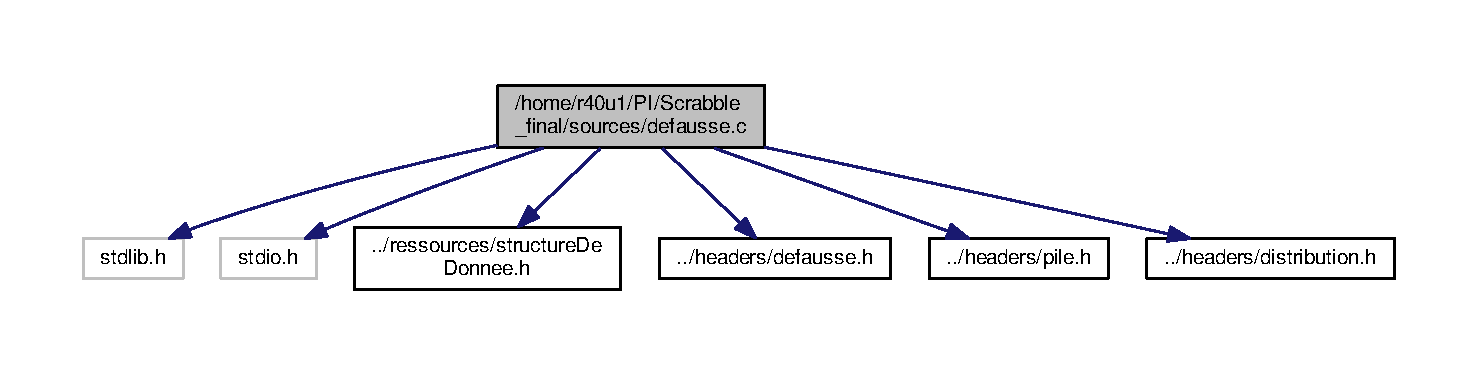
\includegraphics[width=350pt]{defausse_8c__incl}
\end{center}
\end{figure}
\subsection*{Functions}
\begin{DoxyCompactItemize}
\item 
void \hyperlink{defausse_8c_a301ae4fc605cf75a0697c4959201d0fc}{defausse\-Par\-Indice} (\hyperlink{structure_de_donnee_8h_abde700801ddcd10c40bdf389ff5b1494}{Chevalet} chevalet, \hyperlink{structure_de_donnee_8h_aeb2e4c1daa2de38a0efbf9ab87674140}{Pile} $\ast$\hyperlink{interface_8c_a6d4f2018c7ae823808170f38d6f18608}{p\-Pioche}, int \hyperlink{interface_8c_afeef952dff3f63f7fb13ef662475b286}{masque\-Defausse}\mbox{[}7\mbox{]})
\begin{DoxyCompactList}\small\item\em Remet les jetons choisis à un endroit aléatoire de la pioche. \end{DoxyCompactList}\end{DoxyCompactItemize}


\subsection{Detailed Description}
\begin{DoxyVersion}{Version}
1.\-0
\end{DoxyVersion}
Contient la fonction de defausse de lettre pour le programme scrabble 

\subsection{Function Documentation}
\hypertarget{defausse_8c_a301ae4fc605cf75a0697c4959201d0fc}{\index{defausse.\-c@{defausse.\-c}!defausse\-Par\-Indice@{defausse\-Par\-Indice}}
\index{defausse\-Par\-Indice@{defausse\-Par\-Indice}!defausse.c@{defausse.\-c}}
\subsubsection[{defausse\-Par\-Indice}]{\setlength{\rightskip}{0pt plus 5cm}void defausse\-Par\-Indice (
\begin{DoxyParamCaption}
\item[{{\bf Chevalet}}]{chevalet, }
\item[{{\bf Pile} $\ast$}]{p\-Pioche, }
\item[{int}]{masque\-Defausse\mbox{[}7\mbox{]}}
\end{DoxyParamCaption}
)}}\label{defausse_8c_a301ae4fc605cf75a0697c4959201d0fc}


Remet les jetons choisis à un endroit aléatoire de la pioche. 


\begin{DoxyParams}{Parameters}
{\em chevalet} & chevalet dont les lettres sont défaussées \\
\hline
{\em p\-Pioche} & pioche \\
\hline
{\em masque\-Defausse} & \\
\hline
\end{DoxyParams}

\hypertarget{distribution_8c}{\section{/home/r40u1/\-P\-I/\-Scrabble\-\_\-final/sources/distribution.c File Reference}
\label{distribution_8c}\index{/home/r40u1/\-P\-I/\-Scrabble\-\_\-final/sources/distribution.\-c@{/home/r40u1/\-P\-I/\-Scrabble\-\_\-final/sources/distribution.\-c}}
}
{\ttfamily \#include $<$stdlib.\-h$>$}\\*
{\ttfamily \#include $<$stdio.\-h$>$}\\*
{\ttfamily \#include \char`\"{}../ressources/structure\-De\-Donnee.\-h\char`\"{}}\\*
{\ttfamily \#include \char`\"{}../headers/distribution.\-h\char`\"{}}\\*
{\ttfamily \#include \char`\"{}../headers/pile.\-h\char`\"{}}\\*
Include dependency graph for distribution.\-c\-:\nopagebreak
\begin{figure}[H]
\begin{center}
\leavevmode
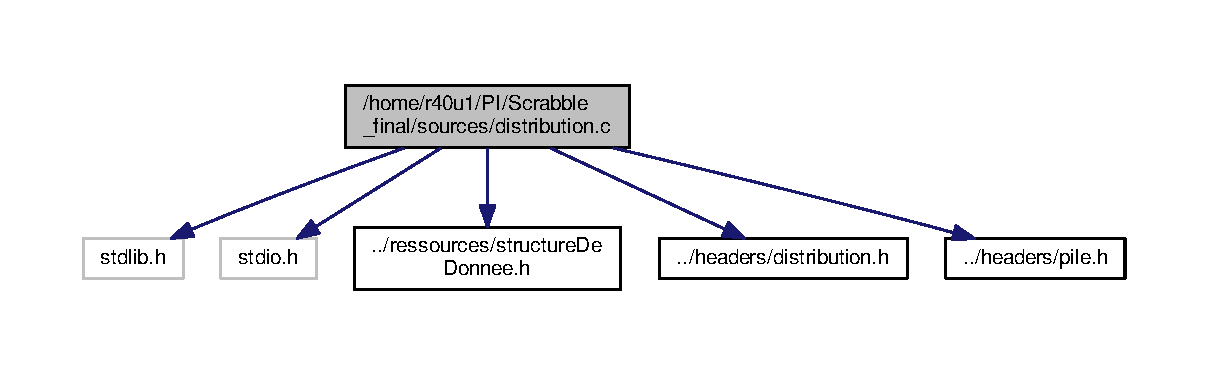
\includegraphics[width=350pt]{distribution_8c__incl}
\end{center}
\end{figure}
\subsection*{Functions}
\begin{DoxyCompactItemize}
\item 
void \hyperlink{distribution_8c_a5a28ffd4625fd10849dac9bde2f695b2}{generation\-Ensemble\-Des\-Jetons} (\hyperlink{struct_jeton}{Jeton} ensemble\-Des\-Jetons\mbox{[}\hyperlink{structure_de_donnee_8h_a71e2e07f0ea54740cb5421e00e77a979}{N\-O\-M\-B\-R\-E\-D\-E\-J\-E\-T\-O\-N}\mbox{]})
\item 
void \hyperlink{distribution_8c_a7d8b638fa86c3426d190350cf0017e33}{empilage\-Aleatoire\-Jeton} (\hyperlink{struct_jeton}{Jeton} ensemble\-Des\-Jetons\mbox{[}\hyperlink{structure_de_donnee_8h_a71e2e07f0ea54740cb5421e00e77a979}{N\-O\-M\-B\-R\-E\-D\-E\-J\-E\-T\-O\-N}\mbox{]}, int nb\-Jetons\-Restants, \hyperlink{structure_de_donnee_8h_aeb2e4c1daa2de38a0efbf9ab87674140}{Pile} $\ast$\hyperlink{interface_8c_a6d4f2018c7ae823808170f38d6f18608}{p\-Pioche})
\item 
void \hyperlink{distribution_8c_af70a8b10ad052f4abdec999a0a7ac5f6}{distribution\-Jetons} (\hyperlink{structure_de_donnee_8h_aeb2e4c1daa2de38a0efbf9ab87674140}{Pile} $\ast$\hyperlink{interface_8c_a6d4f2018c7ae823808170f38d6f18608}{p\-Pioche}, \hyperlink{structure_de_donnee_8h_abde700801ddcd10c40bdf389ff5b1494}{Chevalet} chevalet)
\item 
void \hyperlink{distribution_8c_ac3ed546272da04bab4c146d514c9f309}{distribution\-Initiale} (\hyperlink{struct_jeton}{Jeton} ensemble\-Des\-Jetons\mbox{[}\hyperlink{structure_de_donnee_8h_a71e2e07f0ea54740cb5421e00e77a979}{N\-O\-M\-B\-R\-E\-D\-E\-J\-E\-T\-O\-N}\mbox{]}, \hyperlink{structure_de_donnee_8h_aeb2e4c1daa2de38a0efbf9ab87674140}{Pile} $\ast$\hyperlink{interface_8c_a6d4f2018c7ae823808170f38d6f18608}{p\-Pioche}, \hyperlink{structure_de_donnee_8h_abde700801ddcd10c40bdf389ff5b1494}{Chevalet} ensemble\-Des\-Chevalets\mbox{[}$\,$\mbox{]}, int \hyperlink{interface_8c_a006645f5fca9c8be4a3a8a6398330060}{nb\-Joueurs})
\end{DoxyCompactItemize}


\subsection{Detailed Description}
\begin{DoxyVersion}{Version}
1.\-0
\end{DoxyVersion}
Contient les fonctions qui gèrent les jetons (génération, distribution, empilement). 

\subsection{Function Documentation}
\hypertarget{distribution_8c_ac3ed546272da04bab4c146d514c9f309}{\index{distribution.\-c@{distribution.\-c}!distribution\-Initiale@{distribution\-Initiale}}
\index{distribution\-Initiale@{distribution\-Initiale}!distribution.c@{distribution.\-c}}
\subsubsection[{distribution\-Initiale}]{\setlength{\rightskip}{0pt plus 5cm}void distribution\-Initiale (
\begin{DoxyParamCaption}
\item[{{\bf Jeton}}]{ensemble\-Des\-Jetons\mbox{[}\-N\-O\-M\-B\-R\-E\-D\-E\-J\-E\-T\-O\-N\mbox{]}, }
\item[{{\bf Pile} $\ast$}]{p\-Pioche, }
\item[{{\bf Chevalet}}]{ensemble\-Des\-Chevalets\mbox{[}$\,$\mbox{]}, }
\item[{int}]{nb\-Joueurs}
\end{DoxyParamCaption}
)}}\label{distribution_8c_ac3ed546272da04bab4c146d514c9f309}
Intitialisation des chevalets des joueurs (appel aux 3 fonctions précédentes) \hypertarget{distribution_8c_af70a8b10ad052f4abdec999a0a7ac5f6}{\index{distribution.\-c@{distribution.\-c}!distribution\-Jetons@{distribution\-Jetons}}
\index{distribution\-Jetons@{distribution\-Jetons}!distribution.c@{distribution.\-c}}
\subsubsection[{distribution\-Jetons}]{\setlength{\rightskip}{0pt plus 5cm}void distribution\-Jetons (
\begin{DoxyParamCaption}
\item[{{\bf Pile} $\ast$}]{p\-Pioche, }
\item[{{\bf Chevalet}}]{chevalet}
\end{DoxyParamCaption}
)}}\label{distribution_8c_af70a8b10ad052f4abdec999a0a7ac5f6}
On distribue le nombre de jetons nécessaires afin de compléter le chevalet du joueur \hypertarget{distribution_8c_a7d8b638fa86c3426d190350cf0017e33}{\index{distribution.\-c@{distribution.\-c}!empilage\-Aleatoire\-Jeton@{empilage\-Aleatoire\-Jeton}}
\index{empilage\-Aleatoire\-Jeton@{empilage\-Aleatoire\-Jeton}!distribution.c@{distribution.\-c}}
\subsubsection[{empilage\-Aleatoire\-Jeton}]{\setlength{\rightskip}{0pt plus 5cm}void empilage\-Aleatoire\-Jeton (
\begin{DoxyParamCaption}
\item[{{\bf Jeton}}]{ensemble\-Des\-Jetons\mbox{[}\-N\-O\-M\-B\-R\-E\-D\-E\-J\-E\-T\-O\-N\mbox{]}, }
\item[{int}]{nb\-Jetons\-Restants, }
\item[{{\bf Pile} $\ast$}]{p\-Pioche}
\end{DoxyParamCaption}
)}}\label{distribution_8c_a7d8b638fa86c3426d190350cf0017e33}
Les jetons du tableau sont empilés aléatoirement dans la pioche \hypertarget{distribution_8c_a5a28ffd4625fd10849dac9bde2f695b2}{\index{distribution.\-c@{distribution.\-c}!generation\-Ensemble\-Des\-Jetons@{generation\-Ensemble\-Des\-Jetons}}
\index{generation\-Ensemble\-Des\-Jetons@{generation\-Ensemble\-Des\-Jetons}!distribution.c@{distribution.\-c}}
\subsubsection[{generation\-Ensemble\-Des\-Jetons}]{\setlength{\rightskip}{0pt plus 5cm}void generation\-Ensemble\-Des\-Jetons (
\begin{DoxyParamCaption}
\item[{{\bf Jeton}}]{ensemble\-Des\-Jetons\mbox{[}\-N\-O\-M\-B\-R\-E\-D\-E\-J\-E\-T\-O\-N\mbox{]}}
\end{DoxyParamCaption}
)}}\label{distribution_8c_a5a28ffd4625fd10849dac9bde2f695b2}
Construction du tableau des jetons dans l'ordre alphabétique 
\hypertarget{est_dans_dico_8c}{\section{/home/r40u1/\-P\-I/\-Scrabble\-\_\-final/sources/est\-Dans\-Dico.c File Reference}
\label{est_dans_dico_8c}\index{/home/r40u1/\-P\-I/\-Scrabble\-\_\-final/sources/est\-Dans\-Dico.\-c@{/home/r40u1/\-P\-I/\-Scrabble\-\_\-final/sources/est\-Dans\-Dico.\-c}}
}
{\ttfamily \#include $<$stdlib.\-h$>$}\\*
{\ttfamily \#include $<$stdio.\-h$>$}\\*
{\ttfamily \#include \char`\"{}../ressources/structure\-De\-Donnee.\-h\char`\"{}}\\*
{\ttfamily \#include \char`\"{}../headers/est\-Dans\-Dico.\-h\char`\"{}}\\*
Include dependency graph for est\-Dans\-Dico.\-c\-:\nopagebreak
\begin{figure}[H]
\begin{center}
\leavevmode
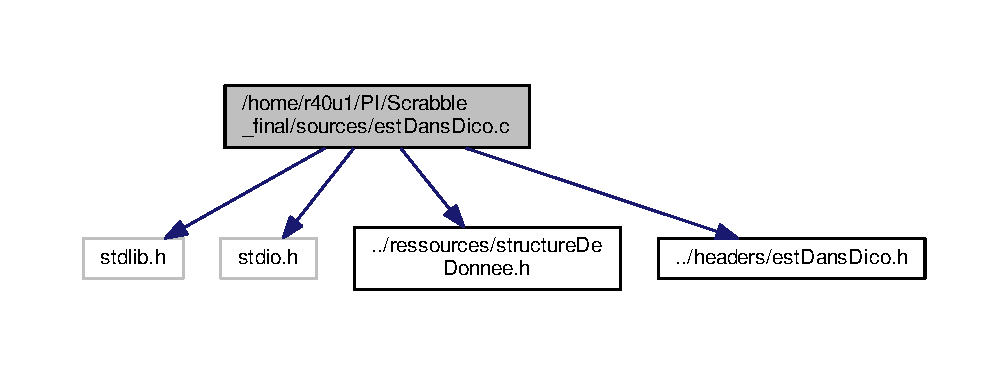
\includegraphics[width=350pt]{est_dans_dico_8c__incl}
\end{center}
\end{figure}
\subsection*{Functions}
\begin{DoxyCompactItemize}
\item 
\hyperlink{structure_de_donnee_8h_a426c0d223e7dc6b87d723c4c0c0e1f58}{Booleen} \hyperlink{est_dans_dico_8c_a1e885dbf9866c7e930fd6eea00b8dd76}{comparer} (char $\ast$mot1, char $\ast$mot2)
\item 
\hyperlink{structure_de_donnee_8h_a426c0d223e7dc6b87d723c4c0c0e1f58}{Booleen} \hyperlink{est_dans_dico_8c_a3bcdca923df984cf2349d6074f2ce000}{est\-Dans\-Dico} (char $\ast$mot)
\end{DoxyCompactItemize}


\subsection{Detailed Description}
\begin{DoxyVersion}{Version}
1.\-0
\end{DoxyVersion}
Programme pour voir si un mot appartient au dictionnaire. 

\subsection{Function Documentation}
\hypertarget{est_dans_dico_8c_a1e885dbf9866c7e930fd6eea00b8dd76}{\index{est\-Dans\-Dico.\-c@{est\-Dans\-Dico.\-c}!comparer@{comparer}}
\index{comparer@{comparer}!estDansDico.c@{est\-Dans\-Dico.\-c}}
\subsubsection[{comparer}]{\setlength{\rightskip}{0pt plus 5cm}{\bf Booleen} comparer (
\begin{DoxyParamCaption}
\item[{char $\ast$}]{mot1, }
\item[{char $\ast$}]{mot2}
\end{DoxyParamCaption}
)}}\label{est_dans_dico_8c_a1e885dbf9866c7e930fd6eea00b8dd76}
retourne V\-R\-A\-I si les deux mots sont identiques \hypertarget{est_dans_dico_8c_a3bcdca923df984cf2349d6074f2ce000}{\index{est\-Dans\-Dico.\-c@{est\-Dans\-Dico.\-c}!est\-Dans\-Dico@{est\-Dans\-Dico}}
\index{est\-Dans\-Dico@{est\-Dans\-Dico}!estDansDico.c@{est\-Dans\-Dico.\-c}}
\subsubsection[{est\-Dans\-Dico}]{\setlength{\rightskip}{0pt plus 5cm}{\bf Booleen} est\-Dans\-Dico (
\begin{DoxyParamCaption}
\item[{char $\ast$}]{mot}
\end{DoxyParamCaption}
)}}\label{est_dans_dico_8c_a3bcdca923df984cf2349d6074f2ce000}
retourne V\-R\-A\-I si le mot se trouve dans le dictionnaire 
\hypertarget{grille_8c}{\section{/home/r40u1/\-P\-I/\-Scrabble\-\_\-final/sources/grille.c File Reference}
\label{grille_8c}\index{/home/r40u1/\-P\-I/\-Scrabble\-\_\-final/sources/grille.\-c@{/home/r40u1/\-P\-I/\-Scrabble\-\_\-final/sources/grille.\-c}}
}
{\ttfamily \#include $<$stdlib.\-h$>$}\\*
{\ttfamily \#include $<$stdio.\-h$>$}\\*
{\ttfamily \#include \char`\"{}../ressources/structure\-De\-Donnee.\-h\char`\"{}}\\*
{\ttfamily \#include \char`\"{}../headers/grille.\-h\char`\"{}}\\*
Include dependency graph for grille.\-c\-:\nopagebreak
\begin{figure}[H]
\begin{center}
\leavevmode
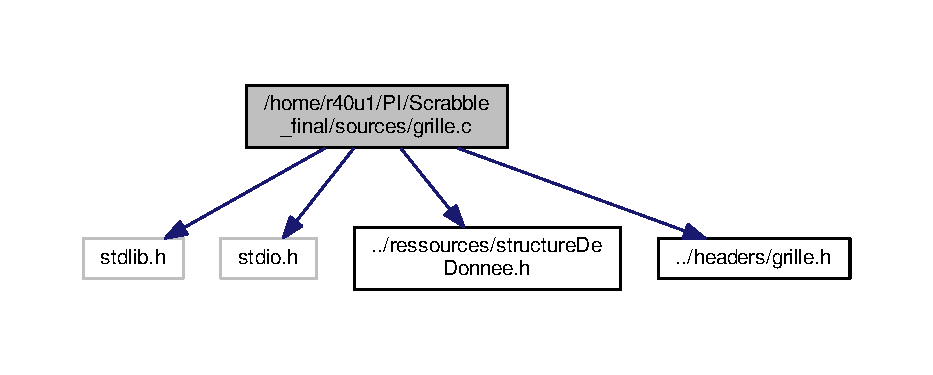
\includegraphics[width=350pt]{grille_8c__incl}
\end{center}
\end{figure}
\subsection*{Functions}
\begin{DoxyCompactItemize}
\item 
void \hyperlink{grille_8c_aea9f328ee16f7d03cd836fa3cfb0d62a}{bonus\-Partiel} (\hyperlink{structure_de_donnee_8h_a4b19d9524b7f293ad87dd6bd9d121b25}{Grille} grille)
\item 
void \hyperlink{grille_8c_a9b2955f028d1c2fd61e5c0bf3c3c3a4d}{symetries} (\hyperlink{structure_de_donnee_8h_a4b19d9524b7f293ad87dd6bd9d121b25}{Grille} grille)
\item 
void \hyperlink{grille_8c_a21f7d6889dc7a0400edc3051a92a65ce}{generer\-Grille} (\hyperlink{structure_de_donnee_8h_a4b19d9524b7f293ad87dd6bd9d121b25}{Grille} $\ast$\hyperlink{interface_8c_a73ce74e635bbc82629b4ca70fea91eb2}{p\-Grille})
\item 
void \hyperlink{grille_8c_a1025b314e1127489285982e0c76d5b67}{afficher\-Grille} (\hyperlink{structure_de_donnee_8h_a4b19d9524b7f293ad87dd6bd9d121b25}{Grille} grille)
\end{DoxyCompactItemize}


\subsection{Detailed Description}
\begin{DoxyVersion}{Version}
1.\-0
\end{DoxyVersion}
Contient les fonctions de génération et d'affichage de la grille. 

\subsection{Function Documentation}
\hypertarget{grille_8c_a1025b314e1127489285982e0c76d5b67}{\index{grille.\-c@{grille.\-c}!afficher\-Grille@{afficher\-Grille}}
\index{afficher\-Grille@{afficher\-Grille}!grille.c@{grille.\-c}}
\subsubsection[{afficher\-Grille}]{\setlength{\rightskip}{0pt plus 5cm}void afficher\-Grille (
\begin{DoxyParamCaption}
\item[{{\bf Grille}}]{grille}
\end{DoxyParamCaption}
)}}\label{grille_8c_a1025b314e1127489285982e0c76d5b67}
affichage de la grille sur le terminal \hypertarget{grille_8c_aea9f328ee16f7d03cd836fa3cfb0d62a}{\index{grille.\-c@{grille.\-c}!bonus\-Partiel@{bonus\-Partiel}}
\index{bonus\-Partiel@{bonus\-Partiel}!grille.c@{grille.\-c}}
\subsubsection[{bonus\-Partiel}]{\setlength{\rightskip}{0pt plus 5cm}void bonus\-Partiel (
\begin{DoxyParamCaption}
\item[{{\bf Grille}}]{grille}
\end{DoxyParamCaption}
)}}\label{grille_8c_aea9f328ee16f7d03cd836fa3cfb0d62a}
Initialisation d'un premier huitième de la grille \hypertarget{grille_8c_a21f7d6889dc7a0400edc3051a92a65ce}{\index{grille.\-c@{grille.\-c}!generer\-Grille@{generer\-Grille}}
\index{generer\-Grille@{generer\-Grille}!grille.c@{grille.\-c}}
\subsubsection[{generer\-Grille}]{\setlength{\rightskip}{0pt plus 5cm}void generer\-Grille (
\begin{DoxyParamCaption}
\item[{{\bf Grille} $\ast$}]{p\-Grille}
\end{DoxyParamCaption}
)}}\label{grille_8c_a21f7d6889dc7a0400edc3051a92a65ce}
génère la grille (combinaison des deux fonctions précédentes \hypertarget{grille_8c_a9b2955f028d1c2fd61e5c0bf3c3c3a4d}{\index{grille.\-c@{grille.\-c}!symetries@{symetries}}
\index{symetries@{symetries}!grille.c@{grille.\-c}}
\subsubsection[{symetries}]{\setlength{\rightskip}{0pt plus 5cm}void symetries (
\begin{DoxyParamCaption}
\item[{{\bf Grille}}]{grille}
\end{DoxyParamCaption}
)}}\label{grille_8c_a9b2955f028d1c2fd61e5c0bf3c3c3a4d}
Obtention de la grille entière par symétries 
\hypertarget{interface_8c}{\section{/home/r40u1/\-P\-I/\-Scrabble\-\_\-final/sources/interface.c File Reference}
\label{interface_8c}\index{/home/r40u1/\-P\-I/\-Scrabble\-\_\-final/sources/interface.\-c@{/home/r40u1/\-P\-I/\-Scrabble\-\_\-final/sources/interface.\-c}}
}
{\ttfamily \#include \char`\"{}../headers/interface.\-h\char`\"{}}\\*
Include dependency graph for interface.\-c\-:\nopagebreak
\begin{figure}[H]
\begin{center}
\leavevmode
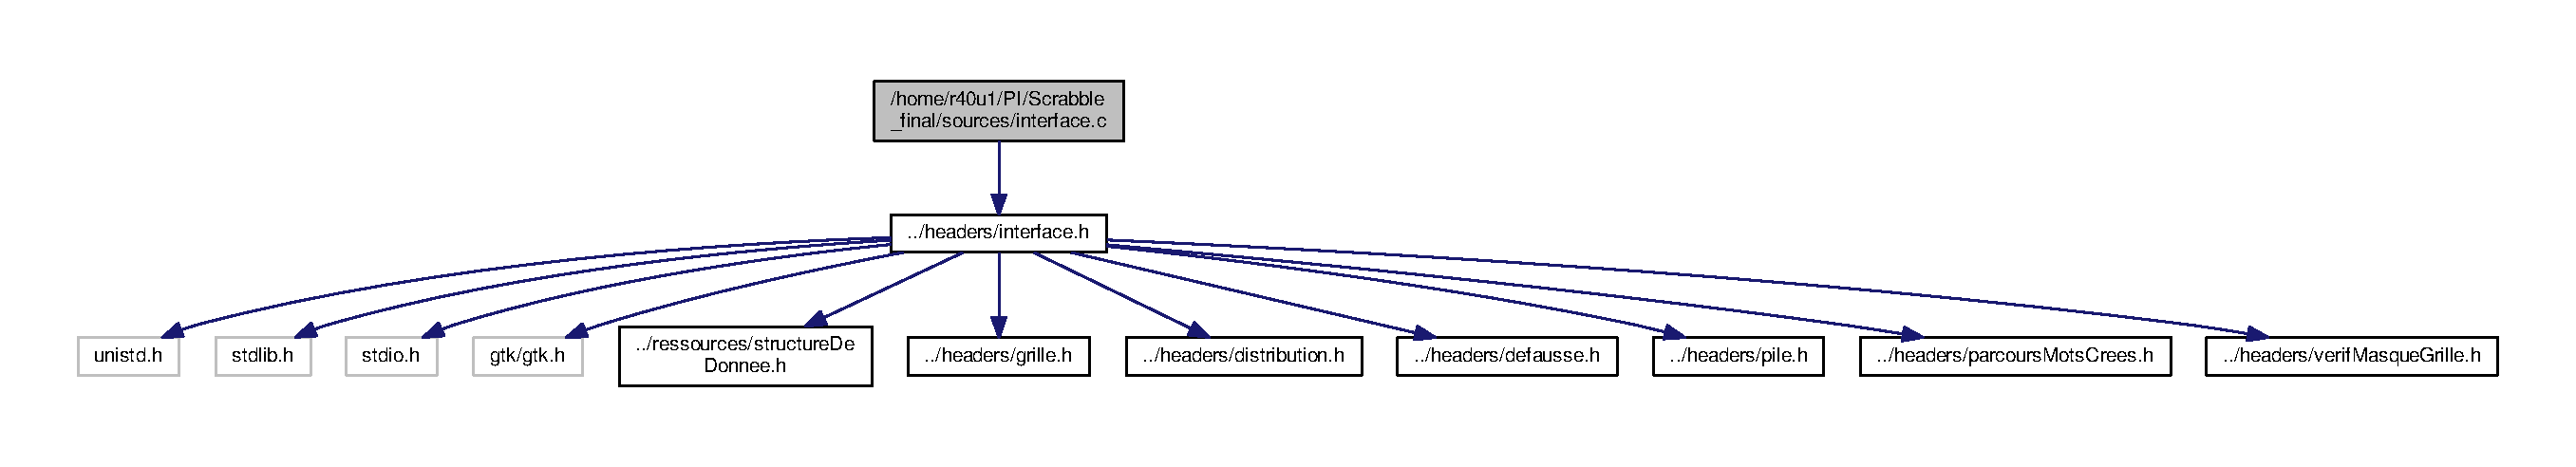
\includegraphics[width=350pt]{interface_8c__incl}
\end{center}
\end{figure}
\subsection*{Functions}
\begin{DoxyCompactItemize}
\item 
int \hyperlink{interface_8c_a3c04138a5bfe5d72780bb7e82a18e627}{main} (int argc, char $\ast$$\ast$argv)
\item 
void \hyperlink{interface_8c_a526a8d1aec28b7ccca94fa2e02e4bd18}{choisir\-Nb\-Joueurs} ()
\item 
void \hyperlink{interface_8c_af4f096a4430a03ce24dfc96254e3134e}{on\-Destroy} (Gtk\-Widget $\ast$p\-Widget, gpointer p\-Data)
\item 
void \hyperlink{interface_8c_ad1473b9c475bd38e7d7ce6eda149da20}{tout\-Fermer} (Gtk\-Widget $\ast$p\-Widget, gpointer p\-Data)
\item 
void \hyperlink{interface_8c_a55fa3c7ab3754e3c68c49530878826c7}{rejouer} (Gtk\-Widget $\ast$p\-Widget, gpointer p\-Data)
\item 
void \hyperlink{interface_8c_a552443357dbe94d4a81110d2e30e4a4f}{on\-Destroy2} (Gtk\-Widget $\ast$p\-Widget, gpointer p\-Data)
\item 
void \hyperlink{interface_8c_a3bdd3a4c0dcf80136881ac584ca28459}{mise\-A\-Jour\-Chevalet} (\hyperlink{struct_image_cliquable}{Image\-Cliquable} \hyperlink{interface_8c_afd3d322d8336128bbf6d36ec762661c2}{p\-Chevalet}\mbox{[}7\mbox{]}, \hyperlink{structure_de_donnee_8h_abde700801ddcd10c40bdf389ff5b1494}{Chevalet} chevalet\-Virtuel)
\item 
void \hyperlink{interface_8c_a826440afda3f0a2fc08db2811ed1e426}{mise\-A\-Jour\-Grille} (\hyperlink{struct_image_cliquable}{Image\-Cliquable} \hyperlink{interface_8c_a240d2f78bb7839f241f70e92912b8f87}{p\-Quadrillage}\mbox{[}15\mbox{]}\mbox{[}15\mbox{]}, \hyperlink{structure_de_donnee_8h_a4b19d9524b7f293ad87dd6bd9d121b25}{Grille} grille)
\item 
void \hyperlink{interface_8c_a1df764e57151185f121c3a1414f9eca5}{nouvelle\-Partie} (Gtk\-Widget $\ast$p\-Widget, gpointer p\-Nb\-Joueurs)
\item 
void \hyperlink{interface_8c_a082c9bde05896c4cf8fadc76da463195}{sauvegarde\-Grille\-Chevalets} (void)
\item 
void \hyperlink{interface_8c_acdb6a13364defbabd5dbcd17cf340d39}{afficher\-Chevalet\-Joueur} (Gtk\-Widget $\ast$p\-Widget, gpointer p\-Data)
\item 
void \hyperlink{interface_8c_a4a8146490f83c8dd3b12d15dba38a129}{selectionner\-Lettre\-Choisie} (Gtk\-Widget $\ast$p\-Lettre\-Choisie, gpointer p\-Data)
\item 
void \hyperlink{interface_8c_a88fc771243ae35fae85bc4744960c921}{deselectionner\-Lettre\-Choisie} (Gtk\-Widget $\ast$p\-Widget, gpointer p\-Data)
\item 
void \hyperlink{interface_8c_aaa1ae69ef2562f9e5a48304b6c053069}{poser\-Lettre\-Choisie} (Gtk\-Widget $\ast$p\-Widget, gpointer p\-Data)
\item 
void \hyperlink{interface_8c_a5e7ffbbfe6b5f3f20c1aa94110a42578}{annuler\-Mot} (Gtk\-Widget $\ast$p\-Widget, gpointer p\-Data)
\item 
void \hyperlink{interface_8c_ace2219ff27db9cc42bd2f8ef2a1c6927}{valider\-Pose} (Gtk\-Widget $\ast$p\-Widget, gpointer p\-Data)
\item 
void \hyperlink{interface_8c_a9a4135ad9f77ef9f5ef05c6f719ef263}{defausser} (Gtk\-Widget $\ast$p\-Widget, gpointer p\-Data)
\item 
void \hyperlink{interface_8c_aefa85ce077ba68d6466ff40ff003e254}{defausser\-Lettre\-Choisie} (Gtk\-Widget $\ast$p\-Widget, gpointer p\-Data)
\item 
void \hyperlink{interface_8c_a848f4a9c0d47cd36d11bf242a509da1e}{annuler\-Defausser\-Lettre\-Choisie} (Gtk\-Widget $\ast$p\-Widget, gpointer p\-Data)
\item 
void \hyperlink{interface_8c_a215247abde0f785768cb4fa6f20c28bd}{valider\-Defausse} (Gtk\-Widget $\ast$p\-Widget, gpointer p\-Data)
\item 
void \hyperlink{interface_8c_abee2513b14c65f04e77e2e5791738c28}{passer\-Tour} (Gtk\-Widget $\ast$p\-Widget, gpointer p\-Data)
\item 
void \hyperlink{interface_8c_a0574bb936d7d1b923cd671de7fe3d31b}{fin\-De\-Partie} ()
\item 
void \hyperlink{interface_8c_acbdd784a6aaf43ec09f8e3a91f8ffe31}{gtk\-\_\-imagecliquable\-\_\-new} (\hyperlink{struct_image_cliquable}{Image\-Cliquable} $\ast$p\-Image\-Cliquable)
\item 
void \hyperlink{interface_8c_a83bbc8a0fb1c878f689795c5d9bb9219}{gtk\-\_\-imagecliquable\-\_\-set\-\_\-image\-\_\-from\-\_\-file} (\hyperlink{struct_image_cliquable}{Image\-Cliquable} $\ast$p\-Image\-Cliquable, char $\ast$file)
\end{DoxyCompactItemize}
\subsection*{Variables}
\begin{DoxyCompactItemize}
\item 
Gtk\-Widget $\ast$ \hyperlink{interface_8c_a084474a38141486428e11731cffad8a7}{p\-Window}
\item 
Gtk\-Widget $\ast$ \hyperlink{interface_8c_af64a0906620ea4401d296d6b2b723317}{p\-Window2}
\item 
Gtk\-Widget $\ast$ \hyperlink{interface_8c_aa206cd3d7bb4c649c0748838f4a8069c}{p\-Table}
\item 
Gtk\-Widget $\ast$ \hyperlink{interface_8c_a6bd4eb82be74dbdd3b84118604317b66}{p\-Zone\-Score}
\item 
Gtk\-Widget $\ast$ \hyperlink{interface_8c_adf695fb5d3716fc9a72d59d617627c0a}{p\-Score\-Box}
\item 
Gtk\-Widget $\ast$ \hyperlink{interface_8c_a73ce74e635bbc82629b4ca70fea91eb2}{p\-Grille}
\item 
\hyperlink{struct_image_cliquable}{Image\-Cliquable} \hyperlink{interface_8c_a240d2f78bb7839f241f70e92912b8f87}{p\-Quadrillage} \mbox{[}15\mbox{]}\mbox{[}15\mbox{]}
\item 
Gtk\-Widget $\ast$ \hyperlink{interface_8c_a0eaa0cf1e0aa86dcec3a087a58f4d2f2}{p\-Zone\-Joueur}
\item 
Gtk\-Widget $\ast$ \hyperlink{interface_8c_a35988b89ee0452a4c15936bebb1a6f9c}{p\-Actions\-Box}
\item 
Gtk\-Widget $\ast$ \hyperlink{interface_8c_adc17e104f9c23e9c99a57cd159b0f1b9}{p\-Annuler}
\item 
Gtk\-Widget $\ast$ \hyperlink{interface_8c_a79bd45d1173e5ec7b08a2e8fcc530e91}{p\-O\-K}
\item 
Gtk\-Widget $\ast$ \hyperlink{interface_8c_a2697870e062b2b23017703843a5680df}{p\-Defausser}
\item 
\hyperlink{struct_image_cliquable}{Image\-Cliquable} \hyperlink{interface_8c_afd3d322d8336128bbf6d36ec762661c2}{p\-Chevalet} \mbox{[}7\mbox{]}
\item 
Gtk\-Widget $\ast$ \hyperlink{interface_8c_a47e00f09d8cb0e0507882bf3ebee96be}{p\-Joueur}
\item 
Gtk\-Widget $\ast$ \hyperlink{interface_8c_ad98762ebfd88b0bff7ec8c3138374992}{p\-Score\-Joueurs} \mbox{[}4\mbox{]}
\item 
Gtk\-Widget $\ast$ \hyperlink{interface_8c_ade66007b6c419c55c5b14507ae0f5157}{p\-Pret}
\item 
int \hyperlink{interface_8c_a006645f5fca9c8be4a3a8a6398330060}{nb\-Joueurs}
\item 
int \hyperlink{interface_8c_ae95f84708dd7abb3a13620a22b7a4fc9}{no\-Joueur} =1
\item 
int \hyperlink{interface_8c_a1f84dff8260c91d60fc679e637d779a8}{nb\-Lettres\-Posees} =0
\item 
int \hyperlink{interface_8c_a8db8fca73724c5e1508f20edcb0dc5e1}{score} \mbox{[}4\mbox{]}
\item 
\hyperlink{structure_de_donnee_8h_a4b19d9524b7f293ad87dd6bd9d121b25}{Grille} $\ast$ \hyperlink{interface_8c_ae6dd73806f726e6dd6003352e1e7d0cd}{p\-Grille\-Virtuelle}
\item 
\hyperlink{structure_de_donnee_8h_abde700801ddcd10c40bdf389ff5b1494}{Chevalet} \hyperlink{interface_8c_ad96aa476e3eec893f54bb4b4dd787942}{ensemble\-Des\-Chevalets\-Virtuels} \mbox{[}4\mbox{]}
\item 
\hyperlink{structure_de_donnee_8h_aeb2e4c1daa2de38a0efbf9ab87674140}{Pile} $\ast$ \hyperlink{interface_8c_a6d4f2018c7ae823808170f38d6f18608}{p\-Pioche}
\item 
\hyperlink{structure_de_donnee_8h_abde700801ddcd10c40bdf389ff5b1494}{Chevalet} \hyperlink{interface_8c_a1cb54014fe843c482cbd5ab5a090be87}{ancien\-Ensemble\-Des\-Chevalets\-Virtuels} \mbox{[}4\mbox{]}
\item 
\hyperlink{structure_de_donnee_8h_a4b19d9524b7f293ad87dd6bd9d121b25}{Grille} \hyperlink{interface_8c_a6bbd455d07c5b38c5ffd4639f03bacf5}{ancienne\-Grille\-Virtuelle}
\item 
int \hyperlink{interface_8c_af982f171c866d7cdd138e7dfcfbd88e6}{indice\-Lettre\-Choisie}
\item 
int \hyperlink{interface_8c_afeef952dff3f63f7fb13ef662475b286}{masque\-Defausse} \mbox{[}7\mbox{]}
\item 
int \hyperlink{interface_8c_ad5bfefafa3d248972817c0259efa829d}{masque\-Grille} \mbox{[}15\mbox{]}\mbox{[}15\mbox{]}
\item 
gulong \hyperlink{interface_8c_acb2be00a5c226498acd832d8697dc1ec}{signaux\-Chevalet} \mbox{[}7\mbox{]} =\{0,0,0,0,0,0,0\}
\item 
gulong \hyperlink{interface_8c_a8d415c94657a5c793a61b19e0a15a3a6}{signal\-O\-K}
\item 
gulong \hyperlink{interface_8c_ab8c29bcdedd24354d722f74c39fbbdb4}{signal\-Fermer\-Fenetre2}
\item 
int \hyperlink{interface_8c_ae13416ca7978932845464be710fab240}{passeurs} \mbox{[}4\mbox{]}
\item 
char \hyperlink{interface_8c_ad3e01a56d5cdbd89e97b9b9346bc1a54}{message} \mbox{[}200\mbox{]}
\end{DoxyCompactItemize}


\subsection{Detailed Description}
\begin{DoxyVersion}{Version}
2.\-0
\end{DoxyVersion}
Contient le programme principal (main) et g�re l'interface graphique 

\subsection{Function Documentation}
\hypertarget{interface_8c_acdb6a13364defbabd5dbcd17cf340d39}{\index{interface.\-c@{interface.\-c}!afficher\-Chevalet\-Joueur@{afficher\-Chevalet\-Joueur}}
\index{afficher\-Chevalet\-Joueur@{afficher\-Chevalet\-Joueur}!interface.c@{interface.\-c}}
\subsubsection[{afficher\-Chevalet\-Joueur}]{\setlength{\rightskip}{0pt plus 5cm}void afficher\-Chevalet\-Joueur (
\begin{DoxyParamCaption}
\item[{Gtk\-Widget $\ast$}]{p\-Widget, }
\item[{gpointer}]{p\-Data}
\end{DoxyParamCaption}
)}}\label{interface_8c_acdb6a13364defbabd5dbcd17cf340d39}
Le joueur est pret, on cree et affiche son chevalet \-: on attend qu'il choisisse un lettre a poser ou qu'il choisisse de se defausser \hypertarget{interface_8c_a848f4a9c0d47cd36d11bf242a509da1e}{\index{interface.\-c@{interface.\-c}!annuler\-Defausser\-Lettre\-Choisie@{annuler\-Defausser\-Lettre\-Choisie}}
\index{annuler\-Defausser\-Lettre\-Choisie@{annuler\-Defausser\-Lettre\-Choisie}!interface.c@{interface.\-c}}
\subsubsection[{annuler\-Defausser\-Lettre\-Choisie}]{\setlength{\rightskip}{0pt plus 5cm}void annuler\-Defausser\-Lettre\-Choisie (
\begin{DoxyParamCaption}
\item[{Gtk\-Widget $\ast$}]{p\-Widget, }
\item[{gpointer}]{p\-Data}
\end{DoxyParamCaption}
)}}\label{interface_8c_a848f4a9c0d47cd36d11bf242a509da1e}
Le joueur ne veut plus defausser cette lettre \hypertarget{interface_8c_a5e7ffbbfe6b5f3f20c1aa94110a42578}{\index{interface.\-c@{interface.\-c}!annuler\-Mot@{annuler\-Mot}}
\index{annuler\-Mot@{annuler\-Mot}!interface.c@{interface.\-c}}
\subsubsection[{annuler\-Mot}]{\setlength{\rightskip}{0pt plus 5cm}void annuler\-Mot (
\begin{DoxyParamCaption}
\item[{Gtk\-Widget $\ast$}]{p\-Widget, }
\item[{gpointer}]{p\-Data}
\end{DoxyParamCaption}
)}}\label{interface_8c_a5e7ffbbfe6b5f3f20c1aa94110a42578}
En cours de depose, le joueur ne veut plus poser son mot \-: on retablit la grille et le chevalet aux valeurs sauvegardees \hypertarget{interface_8c_a526a8d1aec28b7ccca94fa2e02e4bd18}{\index{interface.\-c@{interface.\-c}!choisir\-Nb\-Joueurs@{choisir\-Nb\-Joueurs}}
\index{choisir\-Nb\-Joueurs@{choisir\-Nb\-Joueurs}!interface.c@{interface.\-c}}
\subsubsection[{choisir\-Nb\-Joueurs}]{\setlength{\rightskip}{0pt plus 5cm}void choisir\-Nb\-Joueurs (
\begin{DoxyParamCaption}
{}
\end{DoxyParamCaption}
)}}\label{interface_8c_a526a8d1aec28b7ccca94fa2e02e4bd18}
Affichage de la fenetre permettant de choisir combien de joueurs vont jouer \-: on attend le choix du joueur \hypertarget{interface_8c_a9a4135ad9f77ef9f5ef05c6f719ef263}{\index{interface.\-c@{interface.\-c}!defausser@{defausser}}
\index{defausser@{defausser}!interface.c@{interface.\-c}}
\subsubsection[{defausser}]{\setlength{\rightskip}{0pt plus 5cm}void defausser (
\begin{DoxyParamCaption}
\item[{Gtk\-Widget $\ast$}]{p\-Widget, }
\item[{gpointer}]{p\-Data}
\end{DoxyParamCaption}
)}}\label{interface_8c_a9a4135ad9f77ef9f5ef05c6f719ef263}
Le joueur souhaite se defausser d'un certain nombre de ses jetons \hypertarget{interface_8c_aefa85ce077ba68d6466ff40ff003e254}{\index{interface.\-c@{interface.\-c}!defausser\-Lettre\-Choisie@{defausser\-Lettre\-Choisie}}
\index{defausser\-Lettre\-Choisie@{defausser\-Lettre\-Choisie}!interface.c@{interface.\-c}}
\subsubsection[{defausser\-Lettre\-Choisie}]{\setlength{\rightskip}{0pt plus 5cm}void defausser\-Lettre\-Choisie (
\begin{DoxyParamCaption}
\item[{Gtk\-Widget $\ast$}]{p\-Widget, }
\item[{gpointer}]{p\-Data}
\end{DoxyParamCaption}
)}}\label{interface_8c_aefa85ce077ba68d6466ff40ff003e254}
Le joueur a choisit une lettre a defausser \hypertarget{interface_8c_a88fc771243ae35fae85bc4744960c921}{\index{interface.\-c@{interface.\-c}!deselectionner\-Lettre\-Choisie@{deselectionner\-Lettre\-Choisie}}
\index{deselectionner\-Lettre\-Choisie@{deselectionner\-Lettre\-Choisie}!interface.c@{interface.\-c}}
\subsubsection[{deselectionner\-Lettre\-Choisie}]{\setlength{\rightskip}{0pt plus 5cm}void deselectionner\-Lettre\-Choisie (
\begin{DoxyParamCaption}
\item[{Gtk\-Widget $\ast$}]{p\-Widget, }
\item[{gpointer}]{p\-Data}
\end{DoxyParamCaption}
)}}\label{interface_8c_a88fc771243ae35fae85bc4744960c921}
Le joueur ne veut plus poser cette lettre \-: on attend qu'il en choisisse une autre \hypertarget{interface_8c_a0574bb936d7d1b923cd671de7fe3d31b}{\index{interface.\-c@{interface.\-c}!fin\-De\-Partie@{fin\-De\-Partie}}
\index{fin\-De\-Partie@{fin\-De\-Partie}!interface.c@{interface.\-c}}
\subsubsection[{fin\-De\-Partie}]{\setlength{\rightskip}{0pt plus 5cm}void fin\-De\-Partie (
\begin{DoxyParamCaption}
{}
\end{DoxyParamCaption}
)}}\label{interface_8c_a0574bb936d7d1b923cd671de7fe3d31b}
Le fin de la partie a ete declenchee \-: on affiche dans une nouvelle fenetre le score ainsi que le numero du gagnant \hypertarget{interface_8c_acbdd784a6aaf43ec09f8e3a91f8ffe31}{\index{interface.\-c@{interface.\-c}!gtk\-\_\-imagecliquable\-\_\-new@{gtk\-\_\-imagecliquable\-\_\-new}}
\index{gtk\-\_\-imagecliquable\-\_\-new@{gtk\-\_\-imagecliquable\-\_\-new}!interface.c@{interface.\-c}}
\subsubsection[{gtk\-\_\-imagecliquable\-\_\-new}]{\setlength{\rightskip}{0pt plus 5cm}void gtk\-\_\-imagecliquable\-\_\-new (
\begin{DoxyParamCaption}
\item[{{\bf Image\-Cliquable} $\ast$}]{p\-Image\-Cliquable}
\end{DoxyParamCaption}
)}}\label{interface_8c_acbdd784a6aaf43ec09f8e3a91f8ffe31}
initialisation d'une image cliquable \hypertarget{interface_8c_a83bbc8a0fb1c878f689795c5d9bb9219}{\index{interface.\-c@{interface.\-c}!gtk\-\_\-imagecliquable\-\_\-set\-\_\-image\-\_\-from\-\_\-file@{gtk\-\_\-imagecliquable\-\_\-set\-\_\-image\-\_\-from\-\_\-file}}
\index{gtk\-\_\-imagecliquable\-\_\-set\-\_\-image\-\_\-from\-\_\-file@{gtk\-\_\-imagecliquable\-\_\-set\-\_\-image\-\_\-from\-\_\-file}!interface.c@{interface.\-c}}
\subsubsection[{gtk\-\_\-imagecliquable\-\_\-set\-\_\-image\-\_\-from\-\_\-file}]{\setlength{\rightskip}{0pt plus 5cm}void gtk\-\_\-imagecliquable\-\_\-set\-\_\-image\-\_\-from\-\_\-file (
\begin{DoxyParamCaption}
\item[{{\bf Image\-Cliquable} $\ast$}]{p\-Image\-Cliquable, }
\item[{char $\ast$}]{file}
\end{DoxyParamCaption}
)}}\label{interface_8c_a83bbc8a0fb1c878f689795c5d9bb9219}
charger une image dans l'imagecliquable \hypertarget{interface_8c_a3c04138a5bfe5d72780bb7e82a18e627}{\index{interface.\-c@{interface.\-c}!main@{main}}
\index{main@{main}!interface.c@{interface.\-c}}
\subsubsection[{main}]{\setlength{\rightskip}{0pt plus 5cm}int main (
\begin{DoxyParamCaption}
\item[{int}]{argc, }
\item[{char $\ast$$\ast$}]{argv}
\end{DoxyParamCaption}
)}}\label{interface_8c_a3c04138a5bfe5d72780bb7e82a18e627}
\hypertarget{interface_8c_a3bdd3a4c0dcf80136881ac584ca28459}{\index{interface.\-c@{interface.\-c}!mise\-A\-Jour\-Chevalet@{mise\-A\-Jour\-Chevalet}}
\index{mise\-A\-Jour\-Chevalet@{mise\-A\-Jour\-Chevalet}!interface.c@{interface.\-c}}
\subsubsection[{mise\-A\-Jour\-Chevalet}]{\setlength{\rightskip}{0pt plus 5cm}void mise\-A\-Jour\-Chevalet (
\begin{DoxyParamCaption}
\item[{{\bf Image\-Cliquable}}]{p\-Chevalet\mbox{[}7\mbox{]}, }
\item[{{\bf Chevalet}}]{chevalet\-Virtuel}
\end{DoxyParamCaption}
)}}\label{interface_8c_a3bdd3a4c0dcf80136881ac584ca28459}
Mise a jour des textes affiches sur les boutons de l'interface graphique au niveau du chevalet affiche \hypertarget{interface_8c_a826440afda3f0a2fc08db2811ed1e426}{\index{interface.\-c@{interface.\-c}!mise\-A\-Jour\-Grille@{mise\-A\-Jour\-Grille}}
\index{mise\-A\-Jour\-Grille@{mise\-A\-Jour\-Grille}!interface.c@{interface.\-c}}
\subsubsection[{mise\-A\-Jour\-Grille}]{\setlength{\rightskip}{0pt plus 5cm}void mise\-A\-Jour\-Grille (
\begin{DoxyParamCaption}
\item[{{\bf Image\-Cliquable}}]{p\-Quadrillage\mbox{[}15\mbox{]}\mbox{[}15\mbox{]}, }
\item[{{\bf Grille}}]{grille}
\end{DoxyParamCaption}
)}}\label{interface_8c_a826440afda3f0a2fc08db2811ed1e426}
Mise a jour des textes affiches sur les boutons de l'interface graphique au niveau de la grille \hypertarget{interface_8c_a1df764e57151185f121c3a1414f9eca5}{\index{interface.\-c@{interface.\-c}!nouvelle\-Partie@{nouvelle\-Partie}}
\index{nouvelle\-Partie@{nouvelle\-Partie}!interface.c@{interface.\-c}}
\subsubsection[{nouvelle\-Partie}]{\setlength{\rightskip}{0pt plus 5cm}void nouvelle\-Partie (
\begin{DoxyParamCaption}
\item[{Gtk\-Widget $\ast$}]{p\-Widget, }
\item[{gpointer}]{p\-Nb\-Joueurs}
\end{DoxyParamCaption}
)}}\label{interface_8c_a1df764e57151185f121c3a1414f9eca5}
Demarrage d'une nouvelle partie \-: creation des fenetres, de tous les boutons. On attend que le 1er joueur soit pret a commencer \hypertarget{interface_8c_af4f096a4430a03ce24dfc96254e3134e}{\index{interface.\-c@{interface.\-c}!on\-Destroy@{on\-Destroy}}
\index{on\-Destroy@{on\-Destroy}!interface.c@{interface.\-c}}
\subsubsection[{on\-Destroy}]{\setlength{\rightskip}{0pt plus 5cm}void on\-Destroy (
\begin{DoxyParamCaption}
\item[{Gtk\-Widget $\ast$}]{p\-Widget, }
\item[{gpointer}]{p\-Data}
\end{DoxyParamCaption}
)}}\label{interface_8c_af4f096a4430a03ce24dfc96254e3134e}
Fermeture de la fenetre en cours \hypertarget{interface_8c_a552443357dbe94d4a81110d2e30e4a4f}{\index{interface.\-c@{interface.\-c}!on\-Destroy2@{on\-Destroy2}}
\index{on\-Destroy2@{on\-Destroy2}!interface.c@{interface.\-c}}
\subsubsection[{on\-Destroy2}]{\setlength{\rightskip}{0pt plus 5cm}void on\-Destroy2 (
\begin{DoxyParamCaption}
\item[{Gtk\-Widget $\ast$}]{p\-Widget, }
\item[{gpointer}]{p\-Data}
\end{DoxyParamCaption}
)}}\label{interface_8c_a552443357dbe94d4a81110d2e30e4a4f}
Fermeture de la fenetre de jeu et retour au choix du nombre de joueur \hypertarget{interface_8c_abee2513b14c65f04e77e2e5791738c28}{\index{interface.\-c@{interface.\-c}!passer\-Tour@{passer\-Tour}}
\index{passer\-Tour@{passer\-Tour}!interface.c@{interface.\-c}}
\subsubsection[{passer\-Tour}]{\setlength{\rightskip}{0pt plus 5cm}void passer\-Tour (
\begin{DoxyParamCaption}
\item[{Gtk\-Widget $\ast$}]{p\-Widget, }
\item[{gpointer}]{p\-Data}
\end{DoxyParamCaption}
)}}\label{interface_8c_abee2513b14c65f04e77e2e5791738c28}
Le joueur ne peut rien faire, il passe son tour, on passe au joueur suivant \hypertarget{interface_8c_aaa1ae69ef2562f9e5a48304b6c053069}{\index{interface.\-c@{interface.\-c}!poser\-Lettre\-Choisie@{poser\-Lettre\-Choisie}}
\index{poser\-Lettre\-Choisie@{poser\-Lettre\-Choisie}!interface.c@{interface.\-c}}
\subsubsection[{poser\-Lettre\-Choisie}]{\setlength{\rightskip}{0pt plus 5cm}void poser\-Lettre\-Choisie (
\begin{DoxyParamCaption}
\item[{Gtk\-Widget $\ast$}]{p\-Widget, }
\item[{gpointer}]{p\-Data}
\end{DoxyParamCaption}
)}}\label{interface_8c_aaa1ae69ef2562f9e5a48304b6c053069}
Le joueur a choisi la case sur laquelle poser la lettre desiree \-: on attend qu'il en choisisse une autre ou qu'il valide son mot (ou qu'il annule) \hypertarget{interface_8c_a55fa3c7ab3754e3c68c49530878826c7}{\index{interface.\-c@{interface.\-c}!rejouer@{rejouer}}
\index{rejouer@{rejouer}!interface.c@{interface.\-c}}
\subsubsection[{rejouer}]{\setlength{\rightskip}{0pt plus 5cm}void rejouer (
\begin{DoxyParamCaption}
\item[{Gtk\-Widget $\ast$}]{p\-Widget, }
\item[{gpointer}]{p\-Data}
\end{DoxyParamCaption}
)}}\label{interface_8c_a55fa3c7ab3754e3c68c49530878826c7}
Fermeture de toutes les fenetres + Reouverture de celle du choix du nombre de joueur \hypertarget{interface_8c_a082c9bde05896c4cf8fadc76da463195}{\index{interface.\-c@{interface.\-c}!sauvegarde\-Grille\-Chevalets@{sauvegarde\-Grille\-Chevalets}}
\index{sauvegarde\-Grille\-Chevalets@{sauvegarde\-Grille\-Chevalets}!interface.c@{interface.\-c}}
\subsubsection[{sauvegarde\-Grille\-Chevalets}]{\setlength{\rightskip}{0pt plus 5cm}void sauvegarde\-Grille\-Chevalets (
\begin{DoxyParamCaption}
\item[{void}]{}
\end{DoxyParamCaption}
)}}\label{interface_8c_a082c9bde05896c4cf8fadc76da463195}
On sauvegarde la grille et le chevalet au cas ou le joueur voudrait annuler son depot de lettre (ou si son mot n'existe pas etc) \hypertarget{interface_8c_a4a8146490f83c8dd3b12d15dba38a129}{\index{interface.\-c@{interface.\-c}!selectionner\-Lettre\-Choisie@{selectionner\-Lettre\-Choisie}}
\index{selectionner\-Lettre\-Choisie@{selectionner\-Lettre\-Choisie}!interface.c@{interface.\-c}}
\subsubsection[{selectionner\-Lettre\-Choisie}]{\setlength{\rightskip}{0pt plus 5cm}void selectionner\-Lettre\-Choisie (
\begin{DoxyParamCaption}
\item[{Gtk\-Widget $\ast$}]{p\-Lettre\-Choisie, }
\item[{gpointer}]{p\-Data}
\end{DoxyParamCaption}
)}}\label{interface_8c_a4a8146490f83c8dd3b12d15dba38a129}
Le joueur a clique sur la lettre qu'il veut poser \-: on attend qu'il choisisse ou la poser (ou qu'il annule) \hypertarget{interface_8c_ad1473b9c475bd38e7d7ce6eda149da20}{\index{interface.\-c@{interface.\-c}!tout\-Fermer@{tout\-Fermer}}
\index{tout\-Fermer@{tout\-Fermer}!interface.c@{interface.\-c}}
\subsubsection[{tout\-Fermer}]{\setlength{\rightskip}{0pt plus 5cm}void tout\-Fermer (
\begin{DoxyParamCaption}
\item[{Gtk\-Widget $\ast$}]{p\-Widget, }
\item[{gpointer}]{p\-Data}
\end{DoxyParamCaption}
)}}\label{interface_8c_ad1473b9c475bd38e7d7ce6eda149da20}
Fermeture de toutes les fenetres \hypertarget{interface_8c_a215247abde0f785768cb4fa6f20c28bd}{\index{interface.\-c@{interface.\-c}!valider\-Defausse@{valider\-Defausse}}
\index{valider\-Defausse@{valider\-Defausse}!interface.c@{interface.\-c}}
\subsubsection[{valider\-Defausse}]{\setlength{\rightskip}{0pt plus 5cm}void valider\-Defausse (
\begin{DoxyParamCaption}
\item[{Gtk\-Widget $\ast$}]{p\-Widget, }
\item[{gpointer}]{p\-Data}
\end{DoxyParamCaption}
)}}\label{interface_8c_a215247abde0f785768cb4fa6f20c28bd}
Le joueur valide son choix de lettres a defausser, on lui en distribue d'autres et on passe au joueur suivant \hypertarget{interface_8c_ace2219ff27db9cc42bd2f8ef2a1c6927}{\index{interface.\-c@{interface.\-c}!valider\-Pose@{valider\-Pose}}
\index{valider\-Pose@{valider\-Pose}!interface.c@{interface.\-c}}
\subsubsection[{valider\-Pose}]{\setlength{\rightskip}{0pt plus 5cm}void valider\-Pose (
\begin{DoxyParamCaption}
\item[{Gtk\-Widget $\ast$}]{p\-Widget, }
\item[{gpointer}]{p\-Data}
\end{DoxyParamCaption}
)}}\label{interface_8c_ace2219ff27db9cc42bd2f8ef2a1c6927}
Le joueur valide son mot \-: on verifie que tout est bon sinon on restaure au chevalet et a la grille sauvegardee 

\subsection{Variable Documentation}
\hypertarget{interface_8c_a1cb54014fe843c482cbd5ab5a090be87}{\index{interface.\-c@{interface.\-c}!ancien\-Ensemble\-Des\-Chevalets\-Virtuels@{ancien\-Ensemble\-Des\-Chevalets\-Virtuels}}
\index{ancien\-Ensemble\-Des\-Chevalets\-Virtuels@{ancien\-Ensemble\-Des\-Chevalets\-Virtuels}!interface.c@{interface.\-c}}
\subsubsection[{ancien\-Ensemble\-Des\-Chevalets\-Virtuels}]{\setlength{\rightskip}{0pt plus 5cm}{\bf Chevalet} ancien\-Ensemble\-Des\-Chevalets\-Virtuels\mbox{[}4\mbox{]}}}\label{interface_8c_a1cb54014fe843c482cbd5ab5a090be87}
emplacement pour sauvegarder les chevalets \hypertarget{interface_8c_a6bbd455d07c5b38c5ffd4639f03bacf5}{\index{interface.\-c@{interface.\-c}!ancienne\-Grille\-Virtuelle@{ancienne\-Grille\-Virtuelle}}
\index{ancienne\-Grille\-Virtuelle@{ancienne\-Grille\-Virtuelle}!interface.c@{interface.\-c}}
\subsubsection[{ancienne\-Grille\-Virtuelle}]{\setlength{\rightskip}{0pt plus 5cm}{\bf Grille} ancienne\-Grille\-Virtuelle}}\label{interface_8c_a6bbd455d07c5b38c5ffd4639f03bacf5}
emplacement pour sauvegarder la grille \hypertarget{interface_8c_ad96aa476e3eec893f54bb4b4dd787942}{\index{interface.\-c@{interface.\-c}!ensemble\-Des\-Chevalets\-Virtuels@{ensemble\-Des\-Chevalets\-Virtuels}}
\index{ensemble\-Des\-Chevalets\-Virtuels@{ensemble\-Des\-Chevalets\-Virtuels}!interface.c@{interface.\-c}}
\subsubsection[{ensemble\-Des\-Chevalets\-Virtuels}]{\setlength{\rightskip}{0pt plus 5cm}{\bf Chevalet} ensemble\-Des\-Chevalets\-Virtuels\mbox{[}4\mbox{]}}}\label{interface_8c_ad96aa476e3eec893f54bb4b4dd787942}
idem avec les chevalets \hypertarget{interface_8c_af982f171c866d7cdd138e7dfcfbd88e6}{\index{interface.\-c@{interface.\-c}!indice\-Lettre\-Choisie@{indice\-Lettre\-Choisie}}
\index{indice\-Lettre\-Choisie@{indice\-Lettre\-Choisie}!interface.c@{interface.\-c}}
\subsubsection[{indice\-Lettre\-Choisie}]{\setlength{\rightskip}{0pt plus 5cm}int indice\-Lettre\-Choisie}}\label{interface_8c_af982f171c866d7cdd138e7dfcfbd88e6}
indice du jeton choisi par le joueur sur son chevalet \hypertarget{interface_8c_afeef952dff3f63f7fb13ef662475b286}{\index{interface.\-c@{interface.\-c}!masque\-Defausse@{masque\-Defausse}}
\index{masque\-Defausse@{masque\-Defausse}!interface.c@{interface.\-c}}
\subsubsection[{masque\-Defausse}]{\setlength{\rightskip}{0pt plus 5cm}int masque\-Defausse\mbox{[}7\mbox{]}}}\label{interface_8c_afeef952dff3f63f7fb13ef662475b286}
vaut 1 si la lettre correspondante du chevalet du joueur actuelle doit etre defaussee \hypertarget{interface_8c_ad5bfefafa3d248972817c0259efa829d}{\index{interface.\-c@{interface.\-c}!masque\-Grille@{masque\-Grille}}
\index{masque\-Grille@{masque\-Grille}!interface.c@{interface.\-c}}
\subsubsection[{masque\-Grille}]{\setlength{\rightskip}{0pt plus 5cm}int masque\-Grille\mbox{[}15\mbox{]}\mbox{[}15\mbox{]}}}\label{interface_8c_ad5bfefafa3d248972817c0259efa829d}
vaut 1 si la case correspondante sur la grille doit recevoir une lettre \hypertarget{interface_8c_ad3e01a56d5cdbd89e97b9b9346bc1a54}{\index{interface.\-c@{interface.\-c}!message@{message}}
\index{message@{message}!interface.c@{interface.\-c}}
\subsubsection[{message}]{\setlength{\rightskip}{0pt plus 5cm}char message\mbox{[}200\mbox{]}}}\label{interface_8c_ad3e01a56d5cdbd89e97b9b9346bc1a54}
contient d'eventuels messages d'erreurs (ex \-: \char`\"{}\-E\-R\-R\-E\-U\-R -\/ Votre mot doit passer par la case centrale\char`\"{}) \hypertarget{interface_8c_a006645f5fca9c8be4a3a8a6398330060}{\index{interface.\-c@{interface.\-c}!nb\-Joueurs@{nb\-Joueurs}}
\index{nb\-Joueurs@{nb\-Joueurs}!interface.c@{interface.\-c}}
\subsubsection[{nb\-Joueurs}]{\setlength{\rightskip}{0pt plus 5cm}int nb\-Joueurs}}\label{interface_8c_a006645f5fca9c8be4a3a8a6398330060}
Le nombre de joueurs \hypertarget{interface_8c_a1f84dff8260c91d60fc679e637d779a8}{\index{interface.\-c@{interface.\-c}!nb\-Lettres\-Posees@{nb\-Lettres\-Posees}}
\index{nb\-Lettres\-Posees@{nb\-Lettres\-Posees}!interface.c@{interface.\-c}}
\subsubsection[{nb\-Lettres\-Posees}]{\setlength{\rightskip}{0pt plus 5cm}int nb\-Lettres\-Posees =0}}\label{interface_8c_a1f84dff8260c91d60fc679e637d779a8}
Le nombre de lettres posees \hypertarget{interface_8c_ae95f84708dd7abb3a13620a22b7a4fc9}{\index{interface.\-c@{interface.\-c}!no\-Joueur@{no\-Joueur}}
\index{no\-Joueur@{no\-Joueur}!interface.c@{interface.\-c}}
\subsubsection[{no\-Joueur}]{\setlength{\rightskip}{0pt plus 5cm}int no\-Joueur =1}}\label{interface_8c_ae95f84708dd7abb3a13620a22b7a4fc9}
Le numero du joueur en cours \hypertarget{interface_8c_a35988b89ee0452a4c15936bebb1a6f9c}{\index{interface.\-c@{interface.\-c}!p\-Actions\-Box@{p\-Actions\-Box}}
\index{p\-Actions\-Box@{p\-Actions\-Box}!interface.c@{interface.\-c}}
\subsubsection[{p\-Actions\-Box}]{\setlength{\rightskip}{0pt plus 5cm}Gtk\-Widget$\ast$ p\-Actions\-Box}}\label{interface_8c_a35988b89ee0452a4c15936bebb1a6f9c}
vbox contenant les boutons p\-Annuler et p\-Defausser \hypertarget{interface_8c_adc17e104f9c23e9c99a57cd159b0f1b9}{\index{interface.\-c@{interface.\-c}!p\-Annuler@{p\-Annuler}}
\index{p\-Annuler@{p\-Annuler}!interface.c@{interface.\-c}}
\subsubsection[{p\-Annuler}]{\setlength{\rightskip}{0pt plus 5cm}Gtk\-Widget$\ast$ p\-Annuler}}\label{interface_8c_adc17e104f9c23e9c99a57cd159b0f1b9}
bouton permettant d'annuler sa pose de mot \hypertarget{interface_8c_ae13416ca7978932845464be710fab240}{\index{interface.\-c@{interface.\-c}!passeurs@{passeurs}}
\index{passeurs@{passeurs}!interface.c@{interface.\-c}}
\subsubsection[{passeurs}]{\setlength{\rightskip}{0pt plus 5cm}int passeurs\mbox{[}4\mbox{]}}}\label{interface_8c_ae13416ca7978932845464be710fab240}
Pour chaque joueur \-: vaut 1 si le joueur a passe son tour (pour la fin de la partie) \hypertarget{interface_8c_afd3d322d8336128bbf6d36ec762661c2}{\index{interface.\-c@{interface.\-c}!p\-Chevalet@{p\-Chevalet}}
\index{p\-Chevalet@{p\-Chevalet}!interface.c@{interface.\-c}}
\subsubsection[{p\-Chevalet}]{\setlength{\rightskip}{0pt plus 5cm}{\bf Image\-Cliquable} p\-Chevalet\mbox{[}7\mbox{]}}}\label{interface_8c_afd3d322d8336128bbf6d36ec762661c2}
tableau de widget$\ast$, il contient les boutons du chevalet \hypertarget{interface_8c_a2697870e062b2b23017703843a5680df}{\index{interface.\-c@{interface.\-c}!p\-Defausser@{p\-Defausser}}
\index{p\-Defausser@{p\-Defausser}!interface.c@{interface.\-c}}
\subsubsection[{p\-Defausser}]{\setlength{\rightskip}{0pt plus 5cm}Gtk\-Widget$\ast$ p\-Defausser}}\label{interface_8c_a2697870e062b2b23017703843a5680df}
bouton permettant de lancer la procedure de defausse \hypertarget{interface_8c_a73ce74e635bbc82629b4ca70fea91eb2}{\index{interface.\-c@{interface.\-c}!p\-Grille@{p\-Grille}}
\index{p\-Grille@{p\-Grille}!interface.c@{interface.\-c}}
\subsubsection[{p\-Grille}]{\setlength{\rightskip}{0pt plus 5cm}Gtk\-Widget$\ast$ p\-Grille}}\label{interface_8c_a73ce74e635bbc82629b4ca70fea91eb2}
table contenant les boutons constituant la grille \hypertarget{interface_8c_ae6dd73806f726e6dd6003352e1e7d0cd}{\index{interface.\-c@{interface.\-c}!p\-Grille\-Virtuelle@{p\-Grille\-Virtuelle}}
\index{p\-Grille\-Virtuelle@{p\-Grille\-Virtuelle}!interface.c@{interface.\-c}}
\subsubsection[{p\-Grille\-Virtuelle}]{\setlength{\rightskip}{0pt plus 5cm}{\bf Grille}$\ast$ p\-Grille\-Virtuelle}}\label{interface_8c_ae6dd73806f726e6dd6003352e1e7d0cd}
la grille telle que le terminal la \char`\"{}voit\char`\"{} (et non pas ce que l'utilisateur voir sur l'interface graphique) \hypertarget{interface_8c_a47e00f09d8cb0e0507882bf3ebee96be}{\index{interface.\-c@{interface.\-c}!p\-Joueur@{p\-Joueur}}
\index{p\-Joueur@{p\-Joueur}!interface.c@{interface.\-c}}
\subsubsection[{p\-Joueur}]{\setlength{\rightskip}{0pt plus 5cm}Gtk\-Widget$\ast$ p\-Joueur}}\label{interface_8c_a47e00f09d8cb0e0507882bf3ebee96be}
label contenant le numero du joueur dont c'est le tour \hypertarget{interface_8c_a79bd45d1173e5ec7b08a2e8fcc530e91}{\index{interface.\-c@{interface.\-c}!p\-O\-K@{p\-O\-K}}
\index{p\-O\-K@{p\-O\-K}!interface.c@{interface.\-c}}
\subsubsection[{p\-O\-K}]{\setlength{\rightskip}{0pt plus 5cm}Gtk\-Widget$\ast$ p\-O\-K}}\label{interface_8c_a79bd45d1173e5ec7b08a2e8fcc530e91}
bouton permettant de lancer la validation du mot pose \hypertarget{interface_8c_a6d4f2018c7ae823808170f38d6f18608}{\index{interface.\-c@{interface.\-c}!p\-Pioche@{p\-Pioche}}
\index{p\-Pioche@{p\-Pioche}!interface.c@{interface.\-c}}
\subsubsection[{p\-Pioche}]{\setlength{\rightskip}{0pt plus 5cm}{\bf Pile}$\ast$ p\-Pioche}}\label{interface_8c_a6d4f2018c7ae823808170f38d6f18608}
La pioche \hypertarget{interface_8c_ade66007b6c419c55c5b14507ae0f5157}{\index{interface.\-c@{interface.\-c}!p\-Pret@{p\-Pret}}
\index{p\-Pret@{p\-Pret}!interface.c@{interface.\-c}}
\subsubsection[{p\-Pret}]{\setlength{\rightskip}{0pt plus 5cm}Gtk\-Widget$\ast$ p\-Pret}}\label{interface_8c_ade66007b6c419c55c5b14507ae0f5157}
bouton utilise lors de la transition entre 2 joueurs \hypertarget{interface_8c_a240d2f78bb7839f241f70e92912b8f87}{\index{interface.\-c@{interface.\-c}!p\-Quadrillage@{p\-Quadrillage}}
\index{p\-Quadrillage@{p\-Quadrillage}!interface.c@{interface.\-c}}
\subsubsection[{p\-Quadrillage}]{\setlength{\rightskip}{0pt plus 5cm}{\bf Image\-Cliquable} p\-Quadrillage\mbox{[}15\mbox{]}\mbox{[}15\mbox{]}}}\label{interface_8c_a240d2f78bb7839f241f70e92912b8f87}
tableau de widget$\ast$, il contient les boutons de la grille \hypertarget{interface_8c_adf695fb5d3716fc9a72d59d617627c0a}{\index{interface.\-c@{interface.\-c}!p\-Score\-Box@{p\-Score\-Box}}
\index{p\-Score\-Box@{p\-Score\-Box}!interface.c@{interface.\-c}}
\subsubsection[{p\-Score\-Box}]{\setlength{\rightskip}{0pt plus 5cm}Gtk\-Widget$\ast$ p\-Score\-Box}}\label{interface_8c_adf695fb5d3716fc9a72d59d617627c0a}
vbox contenant les label affichant le score \hypertarget{interface_8c_ad98762ebfd88b0bff7ec8c3138374992}{\index{interface.\-c@{interface.\-c}!p\-Score\-Joueurs@{p\-Score\-Joueurs}}
\index{p\-Score\-Joueurs@{p\-Score\-Joueurs}!interface.c@{interface.\-c}}
\subsubsection[{p\-Score\-Joueurs}]{\setlength{\rightskip}{0pt plus 5cm}Gtk\-Widget$\ast$ p\-Score\-Joueurs\mbox{[}4\mbox{]}}}\label{interface_8c_ad98762ebfd88b0bff7ec8c3138374992}
label permettant d'afficher le score du joueur \hypertarget{interface_8c_aa206cd3d7bb4c649c0748838f4a8069c}{\index{interface.\-c@{interface.\-c}!p\-Table@{p\-Table}}
\index{p\-Table@{p\-Table}!interface.c@{interface.\-c}}
\subsubsection[{p\-Table}]{\setlength{\rightskip}{0pt plus 5cm}Gtk\-Widget$\ast$ p\-Table}}\label{interface_8c_aa206cd3d7bb4c649c0748838f4a8069c}
table principale de la fenetre de jeu \hypertarget{interface_8c_a084474a38141486428e11731cffad8a7}{\index{interface.\-c@{interface.\-c}!p\-Window@{p\-Window}}
\index{p\-Window@{p\-Window}!interface.c@{interface.\-c}}
\subsubsection[{p\-Window}]{\setlength{\rightskip}{0pt plus 5cm}Gtk\-Widget$\ast$ p\-Window}}\label{interface_8c_a084474a38141486428e11731cffad8a7}
fenetre utilisee pour le choix du nombre de joueur et pour le jeu \hypertarget{interface_8c_af64a0906620ea4401d296d6b2b723317}{\index{interface.\-c@{interface.\-c}!p\-Window2@{p\-Window2}}
\index{p\-Window2@{p\-Window2}!interface.c@{interface.\-c}}
\subsubsection[{p\-Window2}]{\setlength{\rightskip}{0pt plus 5cm}Gtk\-Widget$\ast$ p\-Window2}}\label{interface_8c_af64a0906620ea4401d296d6b2b723317}
fenetre utilisee pour l'affichage du vainqueur \hypertarget{interface_8c_a0eaa0cf1e0aa86dcec3a087a58f4d2f2}{\index{interface.\-c@{interface.\-c}!p\-Zone\-Joueur@{p\-Zone\-Joueur}}
\index{p\-Zone\-Joueur@{p\-Zone\-Joueur}!interface.c@{interface.\-c}}
\subsubsection[{p\-Zone\-Joueur}]{\setlength{\rightskip}{0pt plus 5cm}Gtk\-Widget$\ast$ p\-Zone\-Joueur}}\label{interface_8c_a0eaa0cf1e0aa86dcec3a087a58f4d2f2}
table contenant les widgets de la zone joueur \hypertarget{interface_8c_a6bd4eb82be74dbdd3b84118604317b66}{\index{interface.\-c@{interface.\-c}!p\-Zone\-Score@{p\-Zone\-Score}}
\index{p\-Zone\-Score@{p\-Zone\-Score}!interface.c@{interface.\-c}}
\subsubsection[{p\-Zone\-Score}]{\setlength{\rightskip}{0pt plus 5cm}Gtk\-Widget$\ast$ p\-Zone\-Score}}\label{interface_8c_a6bd4eb82be74dbdd3b84118604317b66}
cadre contenant la zone d'affichage du score \hypertarget{interface_8c_a8db8fca73724c5e1508f20edcb0dc5e1}{\index{interface.\-c@{interface.\-c}!score@{score}}
\index{score@{score}!interface.c@{interface.\-c}}
\subsubsection[{score}]{\setlength{\rightskip}{0pt plus 5cm}int score\mbox{[}4\mbox{]}}}\label{interface_8c_a8db8fca73724c5e1508f20edcb0dc5e1}
Le tableau des 4 joueurs (ou moins) \hypertarget{interface_8c_ab8c29bcdedd24354d722f74c39fbbdb4}{\index{interface.\-c@{interface.\-c}!signal\-Fermer\-Fenetre2@{signal\-Fermer\-Fenetre2}}
\index{signal\-Fermer\-Fenetre2@{signal\-Fermer\-Fenetre2}!interface.c@{interface.\-c}}
\subsubsection[{signal\-Fermer\-Fenetre2}]{\setlength{\rightskip}{0pt plus 5cm}gulong signal\-Fermer\-Fenetre2}}\label{interface_8c_ab8c29bcdedd24354d722f74c39fbbdb4}
identifiant du g\-\_\-signal\-\_\-connect de la fermeture de la fenetre de fin de partie \hypertarget{interface_8c_a8d415c94657a5c793a61b19e0a15a3a6}{\index{interface.\-c@{interface.\-c}!signal\-O\-K@{signal\-O\-K}}
\index{signal\-O\-K@{signal\-O\-K}!interface.c@{interface.\-c}}
\subsubsection[{signal\-O\-K}]{\setlength{\rightskip}{0pt plus 5cm}gulong signal\-O\-K}}\label{interface_8c_a8d415c94657a5c793a61b19e0a15a3a6}
identifiant du g\-\_\-signal\-\_\-connect du bouton O\-K \hypertarget{interface_8c_acb2be00a5c226498acd832d8697dc1ec}{\index{interface.\-c@{interface.\-c}!signaux\-Chevalet@{signaux\-Chevalet}}
\index{signaux\-Chevalet@{signaux\-Chevalet}!interface.c@{interface.\-c}}
\subsubsection[{signaux\-Chevalet}]{\setlength{\rightskip}{0pt plus 5cm}gulong signaux\-Chevalet\mbox{[}7\mbox{]} =\{0,0,0,0,0,0,0\}}}\label{interface_8c_acb2be00a5c226498acd832d8697dc1ec}
identifiants des g\-\_\-signal\-\_\-connect des boutons du chevalets 
\hypertarget{parcours_mots_crees_8c}{\section{/home/r40u1/\-P\-I/\-Scrabble\-\_\-final/sources/parcours\-Mots\-Crees.c File Reference}
\label{parcours_mots_crees_8c}\index{/home/r40u1/\-P\-I/\-Scrabble\-\_\-final/sources/parcours\-Mots\-Crees.\-c@{/home/r40u1/\-P\-I/\-Scrabble\-\_\-final/sources/parcours\-Mots\-Crees.\-c}}
}
{\ttfamily \#include $<$stdio.\-h$>$}\\*
{\ttfamily \#include $<$stdlib.\-h$>$}\\*
{\ttfamily \#include \char`\"{}../ressources/structure\-De\-Donnee.\-h\char`\"{}}\\*
{\ttfamily \#include \char`\"{}../headers/est\-Dans\-Dico.\-h\char`\"{}}\\*
{\ttfamily \#include \char`\"{}../headers/parcours\-Mots\-Crees.\-h\char`\"{}}\\*
Include dependency graph for parcours\-Mots\-Crees.\-c\-:\nopagebreak
\begin{figure}[H]
\begin{center}
\leavevmode
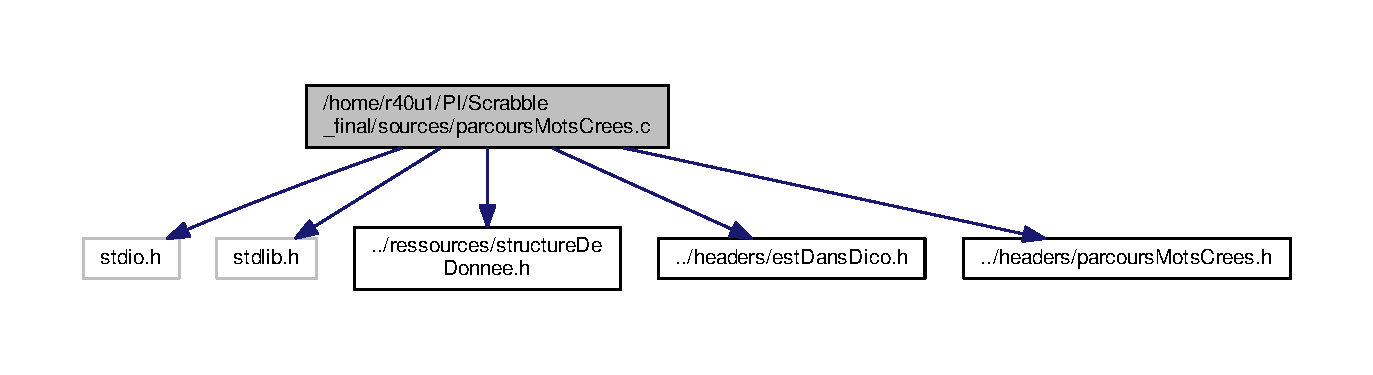
\includegraphics[width=350pt]{parcours_mots_crees_8c__incl}
\end{center}
\end{figure}
\subsection*{Functions}
\begin{DoxyCompactItemize}
\item 
void \hyperlink{parcours_mots_crees_8c_aa81d9b49470738820a7a926be0641490}{calculer\-Score} (int i1, int j1, int i2, int j2, \hyperlink{structure_de_donnee_8h_a4b19d9524b7f293ad87dd6bd9d121b25}{Grille} grille, \hyperlink{structure_de_donnee_8h_a426c0d223e7dc6b87d723c4c0c0e1f58}{Booleen} $\ast$p\-Existence, int $\ast$p\-Score)
\item 
void \hyperlink{parcours_mots_crees_8c_a94bdda82cd125498632aaec642a519e9}{parcours\-Des\-Mots\-Crees} (\hyperlink{structure_de_donnee_8h_a4b19d9524b7f293ad87dd6bd9d121b25}{Grille} grille, char sens, int l0, int c0, int n, \hyperlink{structure_de_donnee_8h_a426c0d223e7dc6b87d723c4c0c0e1f58}{Booleen} $\ast$p\-Tour\-Valide, int $\ast$p\-Score\-Tour, int \hyperlink{interface_8c_ad5bfefafa3d248972817c0259efa829d}{masque\-Grille}\mbox{[}15\mbox{]}\mbox{[}15\mbox{]}, int $\ast$p\-Touche, char \hyperlink{interface_8c_ad3e01a56d5cdbd89e97b9b9346bc1a54}{message}\mbox{[}200\mbox{]})
\end{DoxyCompactItemize}


\subsection{Detailed Description}
\begin{DoxyVersion}{Version}
1.\-0
\end{DoxyVersion}
Contient les fonctions de calcul de score et de vérification de mot. 

\subsection{Function Documentation}
\hypertarget{parcours_mots_crees_8c_aa81d9b49470738820a7a926be0641490}{\index{parcours\-Mots\-Crees.\-c@{parcours\-Mots\-Crees.\-c}!calculer\-Score@{calculer\-Score}}
\index{calculer\-Score@{calculer\-Score}!parcoursMotsCrees.c@{parcours\-Mots\-Crees.\-c}}
\subsubsection[{calculer\-Score}]{\setlength{\rightskip}{0pt plus 5cm}void calculer\-Score (
\begin{DoxyParamCaption}
\item[{int}]{i1, }
\item[{int}]{j1, }
\item[{int}]{i2, }
\item[{int}]{j2, }
\item[{{\bf Grille}}]{grille, }
\item[{{\bf Booleen} $\ast$}]{p\-Existence, }
\item[{int $\ast$}]{p\-Score}
\end{DoxyParamCaption}
)}}\label{parcours_mots_crees_8c_aa81d9b49470738820a7a926be0641490}
à partir des coordonnées d'une suite de lettre, détermine si le mot existe et, si tel est le cas, le nombre de point qu'il rapporte \hypertarget{parcours_mots_crees_8c_a94bdda82cd125498632aaec642a519e9}{\index{parcours\-Mots\-Crees.\-c@{parcours\-Mots\-Crees.\-c}!parcours\-Des\-Mots\-Crees@{parcours\-Des\-Mots\-Crees}}
\index{parcours\-Des\-Mots\-Crees@{parcours\-Des\-Mots\-Crees}!parcoursMotsCrees.c@{parcours\-Mots\-Crees.\-c}}
\subsubsection[{parcours\-Des\-Mots\-Crees}]{\setlength{\rightskip}{0pt plus 5cm}void parcours\-Des\-Mots\-Crees (
\begin{DoxyParamCaption}
\item[{{\bf Grille}}]{grille, }
\item[{char}]{sens, }
\item[{int}]{l0, }
\item[{int}]{c0, }
\item[{int}]{n, }
\item[{{\bf Booleen} $\ast$}]{p\-Tour\-Valide, }
\item[{int $\ast$}]{p\-Score\-Tour, }
\item[{int}]{masque\-Grille\mbox{[}15\mbox{]}\mbox{[}15\mbox{]}, }
\item[{int $\ast$}]{p\-Touche, }
\item[{char}]{message\mbox{[}200\mbox{]}}
\end{DoxyParamCaption}
)}}\label{parcours_mots_crees_8c_a94bdda82cd125498632aaec642a519e9}
recherche tous les mots créés par la dépose des lettres du jouer + détermination de la validité du tour + le cas échéant, du score remporté 
\hypertarget{pile_8c}{\section{/home/r40u1/\-P\-I/\-Scrabble\-\_\-final/sources/pile.c File Reference}
\label{pile_8c}\index{/home/r40u1/\-P\-I/\-Scrabble\-\_\-final/sources/pile.\-c@{/home/r40u1/\-P\-I/\-Scrabble\-\_\-final/sources/pile.\-c}}
}
{\ttfamily \#include $<$stdio.\-h$>$}\\*
{\ttfamily \#include $<$stdlib.\-h$>$}\\*
{\ttfamily \#include \char`\"{}../ressources/structure\-De\-Donnee.\-h\char`\"{}}\\*
{\ttfamily \#include \char`\"{}../headers/pile.\-h\char`\"{}}\\*
Include dependency graph for pile.\-c\-:\nopagebreak
\begin{figure}[H]
\begin{center}
\leavevmode
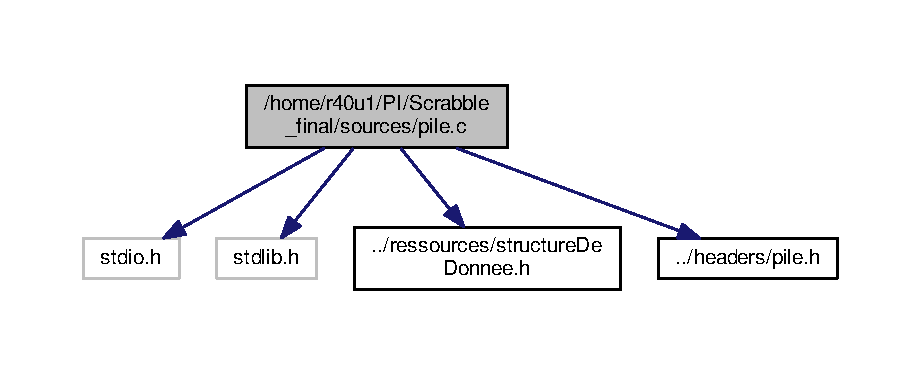
\includegraphics[width=350pt]{pile_8c__incl}
\end{center}
\end{figure}
\subsection*{Functions}
\begin{DoxyCompactItemize}
\item 
\hyperlink{structure_de_donnee_8h_aeb2e4c1daa2de38a0efbf9ab87674140}{Pile} \hyperlink{pile_8c_ad08f6ed24f392bbe68d376207a77c22a}{nouvelle\-Pile} (void)
\item 
void \hyperlink{pile_8c_a4303633aa3fcd700657b6d76a58a9e40}{empiler} (\hyperlink{structure_de_donnee_8h_aeb2e4c1daa2de38a0efbf9ab87674140}{Pile} $\ast$ppile, \hyperlink{struct_jeton}{Jeton} jet)
\item 
\hyperlink{struct_jeton}{Jeton} \hyperlink{pile_8c_a43c3894da262ce42a5ddcafb39e0bdd6}{depiler} (\hyperlink{structure_de_donnee_8h_aeb2e4c1daa2de38a0efbf9ab87674140}{Pile} $\ast$ppile)
\end{DoxyCompactItemize}


\subsection{Detailed Description}
\begin{DoxyVersion}{Version}
1.\-0
\end{DoxyVersion}
Contient des fonctions de gestion de la pile. 

\subsection{Function Documentation}
\hypertarget{pile_8c_a43c3894da262ce42a5ddcafb39e0bdd6}{\index{pile.\-c@{pile.\-c}!depiler@{depiler}}
\index{depiler@{depiler}!pile.c@{pile.\-c}}
\subsubsection[{depiler}]{\setlength{\rightskip}{0pt plus 5cm}{\bf Jeton} depiler (
\begin{DoxyParamCaption}
\item[{{\bf Pile} $\ast$}]{ppile}
\end{DoxyParamCaption}
)}}\label{pile_8c_a43c3894da262ce42a5ddcafb39e0bdd6}
\hypertarget{pile_8c_a4303633aa3fcd700657b6d76a58a9e40}{\index{pile.\-c@{pile.\-c}!empiler@{empiler}}
\index{empiler@{empiler}!pile.c@{pile.\-c}}
\subsubsection[{empiler}]{\setlength{\rightskip}{0pt plus 5cm}void empiler (
\begin{DoxyParamCaption}
\item[{{\bf Pile} $\ast$}]{ppile, }
\item[{{\bf Jeton}}]{jet}
\end{DoxyParamCaption}
)}}\label{pile_8c_a4303633aa3fcd700657b6d76a58a9e40}
\hypertarget{pile_8c_ad08f6ed24f392bbe68d376207a77c22a}{\index{pile.\-c@{pile.\-c}!nouvelle\-Pile@{nouvelle\-Pile}}
\index{nouvelle\-Pile@{nouvelle\-Pile}!pile.c@{pile.\-c}}
\subsubsection[{nouvelle\-Pile}]{\setlength{\rightskip}{0pt plus 5cm}{\bf Pile} nouvelle\-Pile (
\begin{DoxyParamCaption}
\item[{void}]{}
\end{DoxyParamCaption}
)}}\label{pile_8c_ad08f6ed24f392bbe68d376207a77c22a}

\hypertarget{test_defausse_8c}{\section{/home/r40u1/\-P\-I/\-Scrabble\-\_\-final/sources/test\-Defausse.c File Reference}
\label{test_defausse_8c}\index{/home/r40u1/\-P\-I/\-Scrabble\-\_\-final/sources/test\-Defausse.\-c@{/home/r40u1/\-P\-I/\-Scrabble\-\_\-final/sources/test\-Defausse.\-c}}
}
{\ttfamily \#include $<$stdio.\-h$>$}\\*
{\ttfamily \#include $<$stdlib.\-h$>$}\\*
{\ttfamily \#include $<$unistd.\-h$>$}\\*
{\ttfamily \#include \char`\"{}../ressources/structure\-De\-Donnee.\-h\char`\"{}}\\*
{\ttfamily \#include \char`\"{}../headers/distribution.\-h\char`\"{}}\\*
{\ttfamily \#include \char`\"{}../headers/defausse.\-h\char`\"{}}\\*
Include dependency graph for test\-Defausse.\-c\-:\nopagebreak
\begin{figure}[H]
\begin{center}
\leavevmode
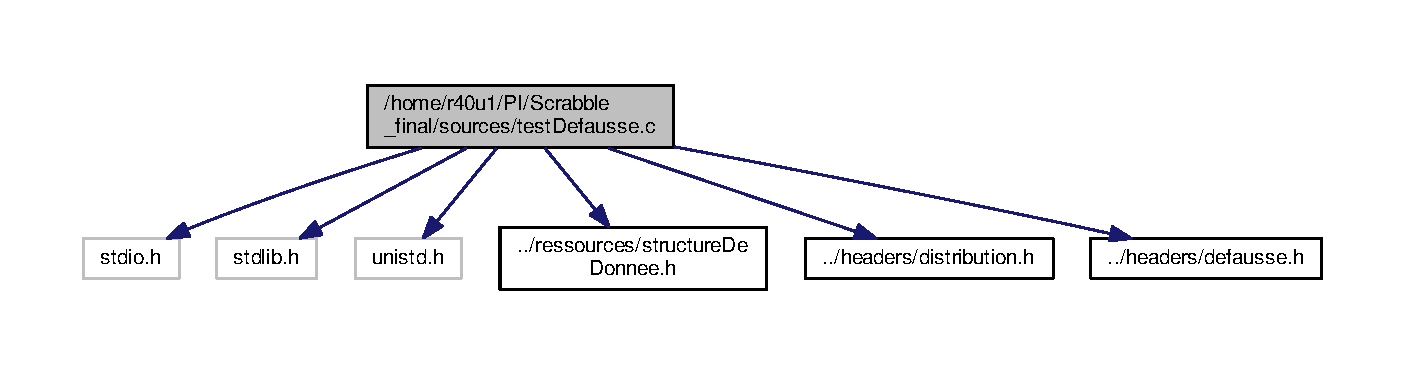
\includegraphics[width=350pt]{test_defausse_8c__incl}
\end{center}
\end{figure}
\subsection*{Functions}
\begin{DoxyCompactItemize}
\item 
void \hyperlink{test_defausse_8c_ad5684c128599f748b3a027e7ef2198e6}{afficher\-Chevalet} (\hyperlink{structure_de_donnee_8h_abde700801ddcd10c40bdf389ff5b1494}{Chevalet} chevalet)
\item 
int \hyperlink{test_defausse_8c_a840291bc02cba5474a4cb46a9b9566fe}{main} (void)
\end{DoxyCompactItemize}


\subsection{Detailed Description}
\begin{DoxyVersion}{Version}
1.\-0
\end{DoxyVersion}
Programme de test de defausse. 

\subsection{Function Documentation}
\hypertarget{test_defausse_8c_ad5684c128599f748b3a027e7ef2198e6}{\index{test\-Defausse.\-c@{test\-Defausse.\-c}!afficher\-Chevalet@{afficher\-Chevalet}}
\index{afficher\-Chevalet@{afficher\-Chevalet}!testDefausse.c@{test\-Defausse.\-c}}
\subsubsection[{afficher\-Chevalet}]{\setlength{\rightskip}{0pt plus 5cm}void afficher\-Chevalet (
\begin{DoxyParamCaption}
\item[{{\bf Chevalet}}]{chevalet}
\end{DoxyParamCaption}
)}}\label{test_defausse_8c_ad5684c128599f748b3a027e7ef2198e6}
\hypertarget{test_defausse_8c_a840291bc02cba5474a4cb46a9b9566fe}{\index{test\-Defausse.\-c@{test\-Defausse.\-c}!main@{main}}
\index{main@{main}!testDefausse.c@{test\-Defausse.\-c}}
\subsubsection[{main}]{\setlength{\rightskip}{0pt plus 5cm}int main (
\begin{DoxyParamCaption}
\item[{void}]{}
\end{DoxyParamCaption}
)}}\label{test_defausse_8c_a840291bc02cba5474a4cb46a9b9566fe}

\hypertarget{test_distribution_8c}{\section{/home/r40u1/\-P\-I/\-Scrabble\-\_\-final/sources/test\-Distribution.c File Reference}
\label{test_distribution_8c}\index{/home/r40u1/\-P\-I/\-Scrabble\-\_\-final/sources/test\-Distribution.\-c@{/home/r40u1/\-P\-I/\-Scrabble\-\_\-final/sources/test\-Distribution.\-c}}
}
{\ttfamily \#include $<$stdio.\-h$>$}\\*
{\ttfamily \#include $<$stdlib.\-h$>$}\\*
{\ttfamily \#include $<$unistd.\-h$>$}\\*
{\ttfamily \#include \char`\"{}../ressources/structure\-De\-Donnee.\-h\char`\"{}}\\*
{\ttfamily \#include \char`\"{}../headers/distribution.\-h\char`\"{}}\\*
Include dependency graph for test\-Distribution.\-c\-:\nopagebreak
\begin{figure}[H]
\begin{center}
\leavevmode
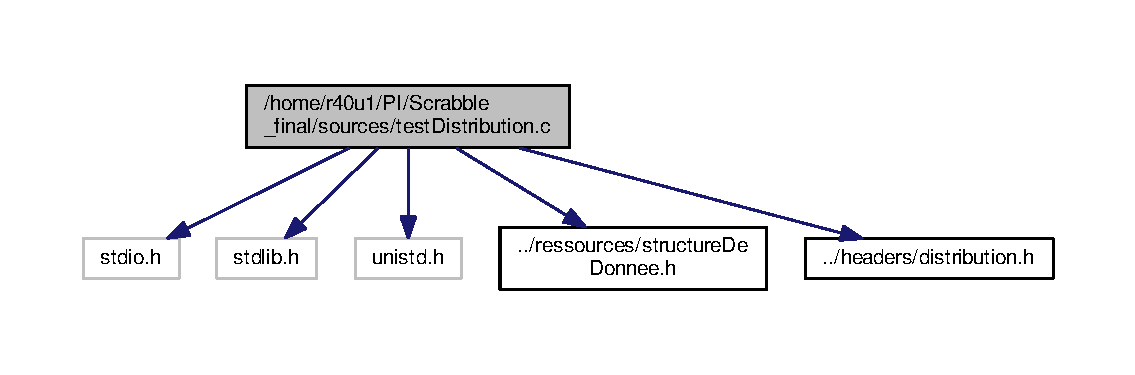
\includegraphics[width=350pt]{test_distribution_8c__incl}
\end{center}
\end{figure}
\subsection*{Functions}
\begin{DoxyCompactItemize}
\item 
int \hyperlink{test_distribution_8c_a840291bc02cba5474a4cb46a9b9566fe}{main} (void)
\end{DoxyCompactItemize}


\subsection{Detailed Description}
\begin{DoxyVersion}{Version}
1.\-0
\end{DoxyVersion}
Programme de test de distribution. 

\subsection{Function Documentation}
\hypertarget{test_distribution_8c_a840291bc02cba5474a4cb46a9b9566fe}{\index{test\-Distribution.\-c@{test\-Distribution.\-c}!main@{main}}
\index{main@{main}!testDistribution.c@{test\-Distribution.\-c}}
\subsubsection[{main}]{\setlength{\rightskip}{0pt plus 5cm}int main (
\begin{DoxyParamCaption}
\item[{void}]{}
\end{DoxyParamCaption}
)}}\label{test_distribution_8c_a840291bc02cba5474a4cb46a9b9566fe}

\hypertarget{test_est_dans_dico_8c}{\section{/home/r40u1/\-P\-I/\-Scrabble\-\_\-final/sources/test\-Est\-Dans\-Dico.c File Reference}
\label{test_est_dans_dico_8c}\index{/home/r40u1/\-P\-I/\-Scrabble\-\_\-final/sources/test\-Est\-Dans\-Dico.\-c@{/home/r40u1/\-P\-I/\-Scrabble\-\_\-final/sources/test\-Est\-Dans\-Dico.\-c}}
}
{\ttfamily \#include $<$stdio.\-h$>$}\\*
{\ttfamily \#include $<$stdlib.\-h$>$}\\*
{\ttfamily \#include \char`\"{}../ressources/structure\-De\-Donnee.\-h\char`\"{}}\\*
{\ttfamily \#include \char`\"{}../headers/est\-Dans\-Dico.\-h\char`\"{}}\\*
Include dependency graph for test\-Est\-Dans\-Dico.\-c\-:\nopagebreak
\begin{figure}[H]
\begin{center}
\leavevmode
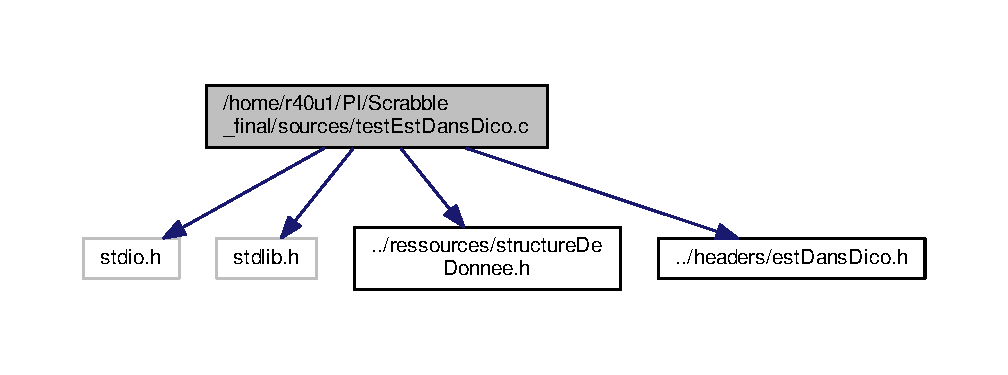
\includegraphics[width=350pt]{test_est_dans_dico_8c__incl}
\end{center}
\end{figure}
\subsection*{Functions}
\begin{DoxyCompactItemize}
\item 
int \hyperlink{test_est_dans_dico_8c_ae66f6b31b5ad750f1fe042a706a4e3d4}{main} ()
\end{DoxyCompactItemize}


\subsection{Detailed Description}
\begin{DoxyVersion}{Version}
1.\-0
\end{DoxyVersion}
Programme de test de vérification de présence d'un mot dans le dictionnaire. 

\subsection{Function Documentation}
\hypertarget{test_est_dans_dico_8c_ae66f6b31b5ad750f1fe042a706a4e3d4}{\index{test\-Est\-Dans\-Dico.\-c@{test\-Est\-Dans\-Dico.\-c}!main@{main}}
\index{main@{main}!testEstDansDico.c@{test\-Est\-Dans\-Dico.\-c}}
\subsubsection[{main}]{\setlength{\rightskip}{0pt plus 5cm}int main (
\begin{DoxyParamCaption}
\item[{void}]{}
\end{DoxyParamCaption}
)}}\label{test_est_dans_dico_8c_ae66f6b31b5ad750f1fe042a706a4e3d4}

\hypertarget{test_grille_8c}{\section{/home/r40u1/\-P\-I/\-Scrabble\-\_\-final/sources/test\-Grille.c File Reference}
\label{test_grille_8c}\index{/home/r40u1/\-P\-I/\-Scrabble\-\_\-final/sources/test\-Grille.\-c@{/home/r40u1/\-P\-I/\-Scrabble\-\_\-final/sources/test\-Grille.\-c}}
}
{\ttfamily \#include $<$stdio.\-h$>$}\\*
{\ttfamily \#include $<$stdlib.\-h$>$}\\*
{\ttfamily \#include \char`\"{}../ressources/structure\-De\-Donnee.\-h\char`\"{}}\\*
{\ttfamily \#include \char`\"{}../headers/grille.\-h\char`\"{}}\\*
Include dependency graph for test\-Grille.\-c\-:\nopagebreak
\begin{figure}[H]
\begin{center}
\leavevmode
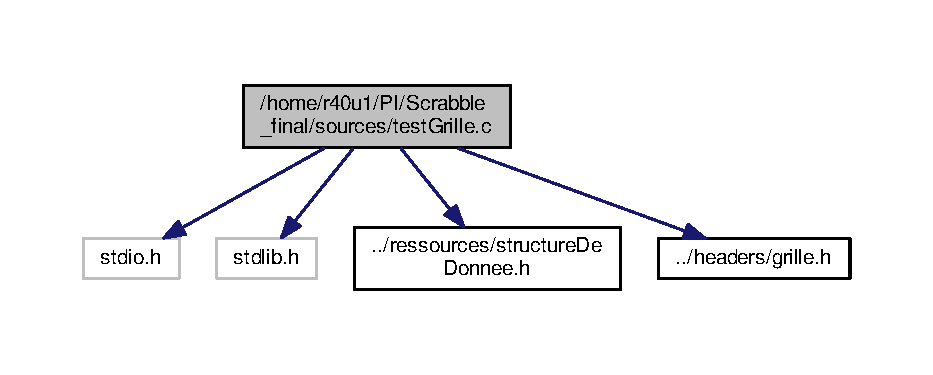
\includegraphics[width=350pt]{test_grille_8c__incl}
\end{center}
\end{figure}
\subsection*{Functions}
\begin{DoxyCompactItemize}
\item 
int \hyperlink{test_grille_8c_a840291bc02cba5474a4cb46a9b9566fe}{main} (void)
\end{DoxyCompactItemize}


\subsection{Detailed Description}
\begin{DoxyVersion}{Version}
1.\-0
\end{DoxyVersion}
Programme de test de génération de grille. 

\subsection{Function Documentation}
\hypertarget{test_grille_8c_a840291bc02cba5474a4cb46a9b9566fe}{\index{test\-Grille.\-c@{test\-Grille.\-c}!main@{main}}
\index{main@{main}!testGrille.c@{test\-Grille.\-c}}
\subsubsection[{main}]{\setlength{\rightskip}{0pt plus 5cm}int main (
\begin{DoxyParamCaption}
\item[{void}]{}
\end{DoxyParamCaption}
)}}\label{test_grille_8c_a840291bc02cba5474a4cb46a9b9566fe}

\hypertarget{verif_masque_grille_8c}{\section{/home/r40u1/\-P\-I/\-Scrabble\-\_\-final/sources/verif\-Masque\-Grille.c File Reference}
\label{verif_masque_grille_8c}\index{/home/r40u1/\-P\-I/\-Scrabble\-\_\-final/sources/verif\-Masque\-Grille.\-c@{/home/r40u1/\-P\-I/\-Scrabble\-\_\-final/sources/verif\-Masque\-Grille.\-c}}
}
{\ttfamily \#include $<$stdlib.\-h$>$}\\*
{\ttfamily \#include $<$stdio.\-h$>$}\\*
{\ttfamily \#include \char`\"{}../ressources/structure\-De\-Donnee.\-h\char`\"{}}\\*
Include dependency graph for verif\-Masque\-Grille.\-c\-:\nopagebreak
\begin{figure}[H]
\begin{center}
\leavevmode
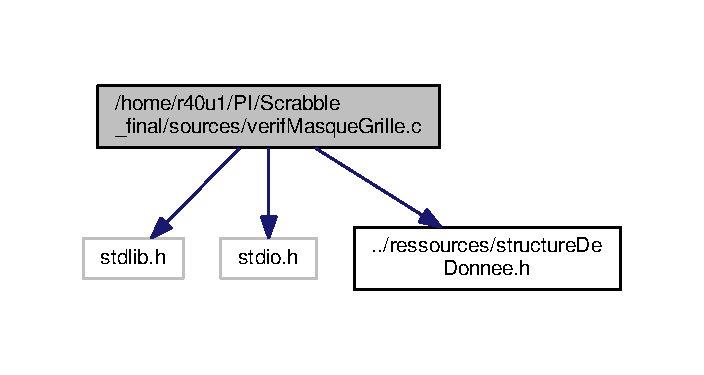
\includegraphics[width=338pt]{verif_masque_grille_8c__incl}
\end{center}
\end{figure}
\subsection*{Functions}
\begin{DoxyCompactItemize}
\item 
int \hyperlink{verif_masque_grille_8c_a6edaa590b57084fef6d331b12a2f6480}{verif\-Masque\-Grille} (\hyperlink{structure_de_donnee_8h_a4b19d9524b7f293ad87dd6bd9d121b25}{Grille} grille, char $\ast$p\-Sens, int $\ast$p\-L0, int $\ast$p\-C0, int $\ast$p\-N, int \hyperlink{interface_8c_ad5bfefafa3d248972817c0259efa829d}{masque\-Grille}\mbox{[}15\mbox{]}\mbox{[}15\mbox{]}, int $\ast$p\-Touche, char \hyperlink{interface_8c_ad3e01a56d5cdbd89e97b9b9346bc1a54}{message}\mbox{[}200\mbox{]})
\end{DoxyCompactItemize}


\subsection{Detailed Description}
\begin{DoxyVersion}{Version}
1.\-0
\end{DoxyVersion}
contient une des fonction de vérification de validité du mot posé. 

\subsection{Function Documentation}
\hypertarget{verif_masque_grille_8c_a6edaa590b57084fef6d331b12a2f6480}{\index{verif\-Masque\-Grille.\-c@{verif\-Masque\-Grille.\-c}!verif\-Masque\-Grille@{verif\-Masque\-Grille}}
\index{verif\-Masque\-Grille@{verif\-Masque\-Grille}!verifMasqueGrille.c@{verif\-Masque\-Grille.\-c}}
\subsubsection[{verif\-Masque\-Grille}]{\setlength{\rightskip}{0pt plus 5cm}int verif\-Masque\-Grille (
\begin{DoxyParamCaption}
\item[{{\bf Grille}}]{grille, }
\item[{char $\ast$}]{p\-Sens, }
\item[{int $\ast$}]{p\-L0, }
\item[{int $\ast$}]{p\-C0, }
\item[{int $\ast$}]{p\-N, }
\item[{int}]{masque\-Grille\mbox{[}15\mbox{]}\mbox{[}15\mbox{]}, }
\item[{int $\ast$}]{p\-Touche, }
\item[{char}]{message\mbox{[}200\mbox{]}}
\end{DoxyParamCaption}
)}}\label{verif_masque_grille_8c_a6edaa590b57084fef6d331b12a2f6480}
Verifie grossièrement si l'emplacement des lettres posees n'est pas incoherent 
%--- End generated contents ---

% Index
\newpage
\phantomsection
\addcontentsline{toc}{chapter}{Index}
\printindex

\end{document}
